% based on a template made by the university of cologne
% http://www.mi.uni-koeln.de/wp-MIEDV/wp-content/uploads/2016/07/LaTeX-Vorlage.zip - 2023-11-02
\documentclass[12pt,a4paper]{scrartcl}

\addtokomafont{sectioning}{\rmfamily}
\usepackage[ngerman]{babel}% deutsches Sprachpaket wird geladen
\usepackage[T1]{fontenc} % westeuropäische Codierung wird verlangt
\usepackage[utf8]{inputenc}% Umlaute werden erlaubt
\usepackage[usenames]{color} % Erlaubt die Benutzung der namen im Farbpaket und deren Änderung
\usepackage{amsmath} % Erweiterung für den Mathe-Satz
\usepackage{amssymb} % alle Zeichen aus msam und msmb werden dargestellt
\usepackage{graphicx} % Graphiken und Bilder können eingebunden werden
%\usepackage{multirow} % erlaubt in einer Spalte einer Tabelle die Felder in mehreren Zeilen zusammenzufassen
\usepackage{enumerate} % erlaubt Nummerierungen
\usepackage{xurl} % Dient zur Auszeichnung von URLs; setzt die Adresse in Schreibmaschinenschrift.
\usepackage[center]{caption}  % Bildunterschrift wird zentriert
%\usepackage{subfigure} % mehrere Bilder können in einer fugure-Umgebung verwendet werden
%\usepackage{longtable} % Diese Umgebung ist ähnlich definiert wie die tabular-Umgebung, erlaubt jedoch mehrseitige Tabellen.
%\usepackage{paralist} % Modifikation der bereits bestehenden Listenumgebungen
\usepackage{lmodern}% Für die Schrift
\usepackage[hidelinks]{hyperref} % Links und Verweise werden innerhalb von PDF Dokumenten erzeugt
%\usepackage{wrapfig} % Das Paket ermöglicht es von Schrift umflossene Bilder und Tabellen einzufügen.
\usepackage{latexsym} % LaTeX-Symbole werden geladen
\usepackage{tikz} % Erlaubt es mit tikz zu zeichnen
\usepackage{tabularx} % Erlaubt Tabellen
\usepackage{algorithm} % Erlaubt Pseudocode
\usepackage{color} % Farbpaket wird geladen
%\usepackage{stmaryrd} % St Mary Road Symbole werden geladen
\usepackage{physics}

\numberwithin{equation}{section} % Nummerierungen der Gleichungen, die durch equation erstellt werden, sind gebunden an die section
\newcommand{\HRule}{\rule{\linewidth}{0.7mm}}
\newcommand{\pu}[1]{\ensuremath{\mathrm{#1}}}

\hypersetup{
  pdftitle={B 2.8},
  pdfcreator={LaTeX via pandoc}}

\setcounter{secnumdepth}{6}
\setcounter{tocdepth}{6}

\hyphenation{Li-thi-um-fluo-rid-Kris-tal-len}
\hyphenation{er-kenn-bar}
\hyphenation{Dop-pel-ätz-me-tho-de}
\hyphenation{Erd-be-schleu-ni-gung}
\hyphenation{Schnitt-flä-che}
\hyphenation{Li-te-ra-tur-wer-te}

\begin{document}
\begin{titlepage}
	\pagestyle{empty}

	\begin{center}

	\textsc{\LARGE Universität zu Köln }\\ [0.4cm]
	\textsc{Mathematisch-Naturwissenschaftliche Fakultät} \\[1.5cm]

	
\includegraphics[width=0.45\textwidth]{../media/uni.jpg}\\[1.5cm]  % Uni-Logo wird geladen

	\textsc{\Large Praktikum~B}\\[2mm]
	\textsc{}\\[10mm]
	\HRule \\[0.4cm]

		{	\Huge \bfseries B 2.8}\\[0.4cm]
			{	\huge \bfseries Versetzungen in Lithiumfluorid}\\[0.3cm]
	
	\HRule \\[3cm]

		\textsc{\Large Catherine Tran } \\[3pt]
		\textsc{\Large Carlo Kleefisch } \\[3pt]
		\textsc{\Large Oliver Filla } \\[3pt]
	\end{center}
\end{titlepage}

\newpage
\tableofcontents
\newpage

\hypertarget{einleitung}{%
\section{Einleitung}\label{einleitung}}

Alle Kristalle haben Kristallbaufehler, die ihre Struktur beeinflussen.
Punktuelle Kristallbaufehler sind für elektrische Eigenschaften
relevant, lineare Kristallbaufehler wie Versetzungen für mechanische
Eigenschaften wie Plastizität und die kritische Fließspannung.

In diesem Versuch werden Versetzungen an der Oberfläche von
Lithiumfluorid-Kristallen mithilfe der Doppelätz-Methode sichtbar
gemacht. Versetzungsbewegungen sind besonders in der
Festkörper-Forschung interessant, da diese Wanderung eine plastische
Verformung ist, aus der man Eigenschaften wie Plastizität und des
Kristall ableiten kann.

\hypertarget{lithiumfluorid}{%
\subsection{Lithiumfluorid}\label{lithiumfluorid}}

Lithiumfluorid ($\mathrm{LiF}$) ist ein ionischer Kristall. Dies
bedeutet, der Kristall wird durch elektrostatische Wechselwirkung
entgegengesetzt geladener Ionen zusammengehalten. $\mathrm{LiF}$
hat eine sehr hohe Gitterenergie von $1034\mathrm{\,\frac{kJ}{mol}}$,
was an den kleinen Ionenradien des Lithiumkations und des Fluoridanions
liegt.

Daher ist es gut für unseren Versuch geeignet, weil
Versetzungswanderungen bei großem Druck durch eine Presse auftreten,
ohne dass die Gitterstruktur großflächig zerstört wird. Stattdessen
gleitet nur ein Teil der Struktur.

Die Gitterstruktur von $\mathrm{LiF}$ entspricht der von
Natriumchlorid mit einer flächenzentriert-kubischen Gitterstruktur und
einer zweiatomigen Basis. Gitterkonstante von $\mathrm{LiF}$ beträgt
$a=0.402\mathrm{\,nm}\pm 1 \cdot 10^{-7} \mathrm{\, \mu m}$. \cite{Uni}

\hypertarget{doppeluxe4tzmethode}{%
\subsection{Doppelätzmethode}\label{doppeluxe4tzmethode}}

Zur Messung von Versetzungsbewegungen wird in diesem Versuch die
Doppelätzmethode angewandt. Sie besteht aus zwei Ätzdurchgängen, um eine
erste Versetzung und anschließend eine Versetzungsbewegung verzeichnen
zu können.

Versetzungen verschiedener Orientierung oder Typen behindern sich
gegenseitig, die reduzierte Mobilität resultiert in einer Ansammlung von
Versetzungshaufen. Diese Ansammlung staut sich an Korngrenzen auf.

Alte Versetzungsstellen sind daran zu erkennen, dass sie dichter
und definierter sind. Die Bewegung wird durch die Messung des Abstand
des letzten Versetzungspunktes nach der ersten Messung und der neuen
Versetzungsstellen bestimmt.

Mithilfe der Bewegungsrichtung und Geschwindigkeit können die
Gleitebene, das Gleitsystem und somit die Versetzungsart bestimmt
werden.

\newpage
\hypertarget{theoretische-grundlagen}{%
\section{Theoretische Grundlagen}\label{theoretische-grundlagen}}

\hypertarget{kuxfcrzester-burgers-vektor-in-mathrmlif}{%
\subsection{\texorpdfstring{kürzester Burgers-Vektor in
$\mathrm{LiF}$}{kürzester Burgers-Vektor in \textbackslash mathrm\{LiF\}}}\label{kuxfcrzester-burgers-vektor-in-mathrmlif}}

Der kürzeste Burgers-Vektor $\vec{b}_\mathrm{min}$ in $\mathrm{LiF}$
ist der $[\frac{1}{2}\,0\,\frac{1}{2}]$ Vektor in der $\expval{1\,1\,0}$ Richtung. Seine Länge bestimmt sich wie folgt durch die Gitterkonstante $a$. \cite{Uni}
\begin{eqnarray}
    \left|\vec{b}_\mathrm{min}\right|
        &=& \frac{1}{2} \cdot \sqrt{a^2 + a^2} \\
        &=& \frac{1}{2} \sqrt{2} a \\
        &=& \frac{a}{\sqrt{2}}
\end{eqnarray}

\noindent
Die Energie einer Versetzung ist proportional zum Quadrat des
Burgers-Vektors. Ein Defekt mit einem längeren Burgers-Vektor benötigt
daher eine viel größeren Energie, was Versetzungen mit längeren
Burgers-Vektoren sehr viel unwahrscheinlicher macht.

Aufgrund der sich abwechselnden Lithium- und Fluoratome in den
Richtungen $\expval{1\,0\,0}$ und $\expval{1\,1\,1}$ sind die
Burgers-Vektoren in diesen Richtungen doppelt so lang, da sie immer
zwischen gleichen Atomen liegen. Der Burgers-Vektor in der
$\expval{1\,0\,0}$-Richtung ist davon nicht betroffen und stellt sich
dadurch als der kürzeste heraus. Dies ist in Abbildung \ref{abb:LiF Kristallgitter} ersichtlich.

\begin{figure}[ht]
\centering
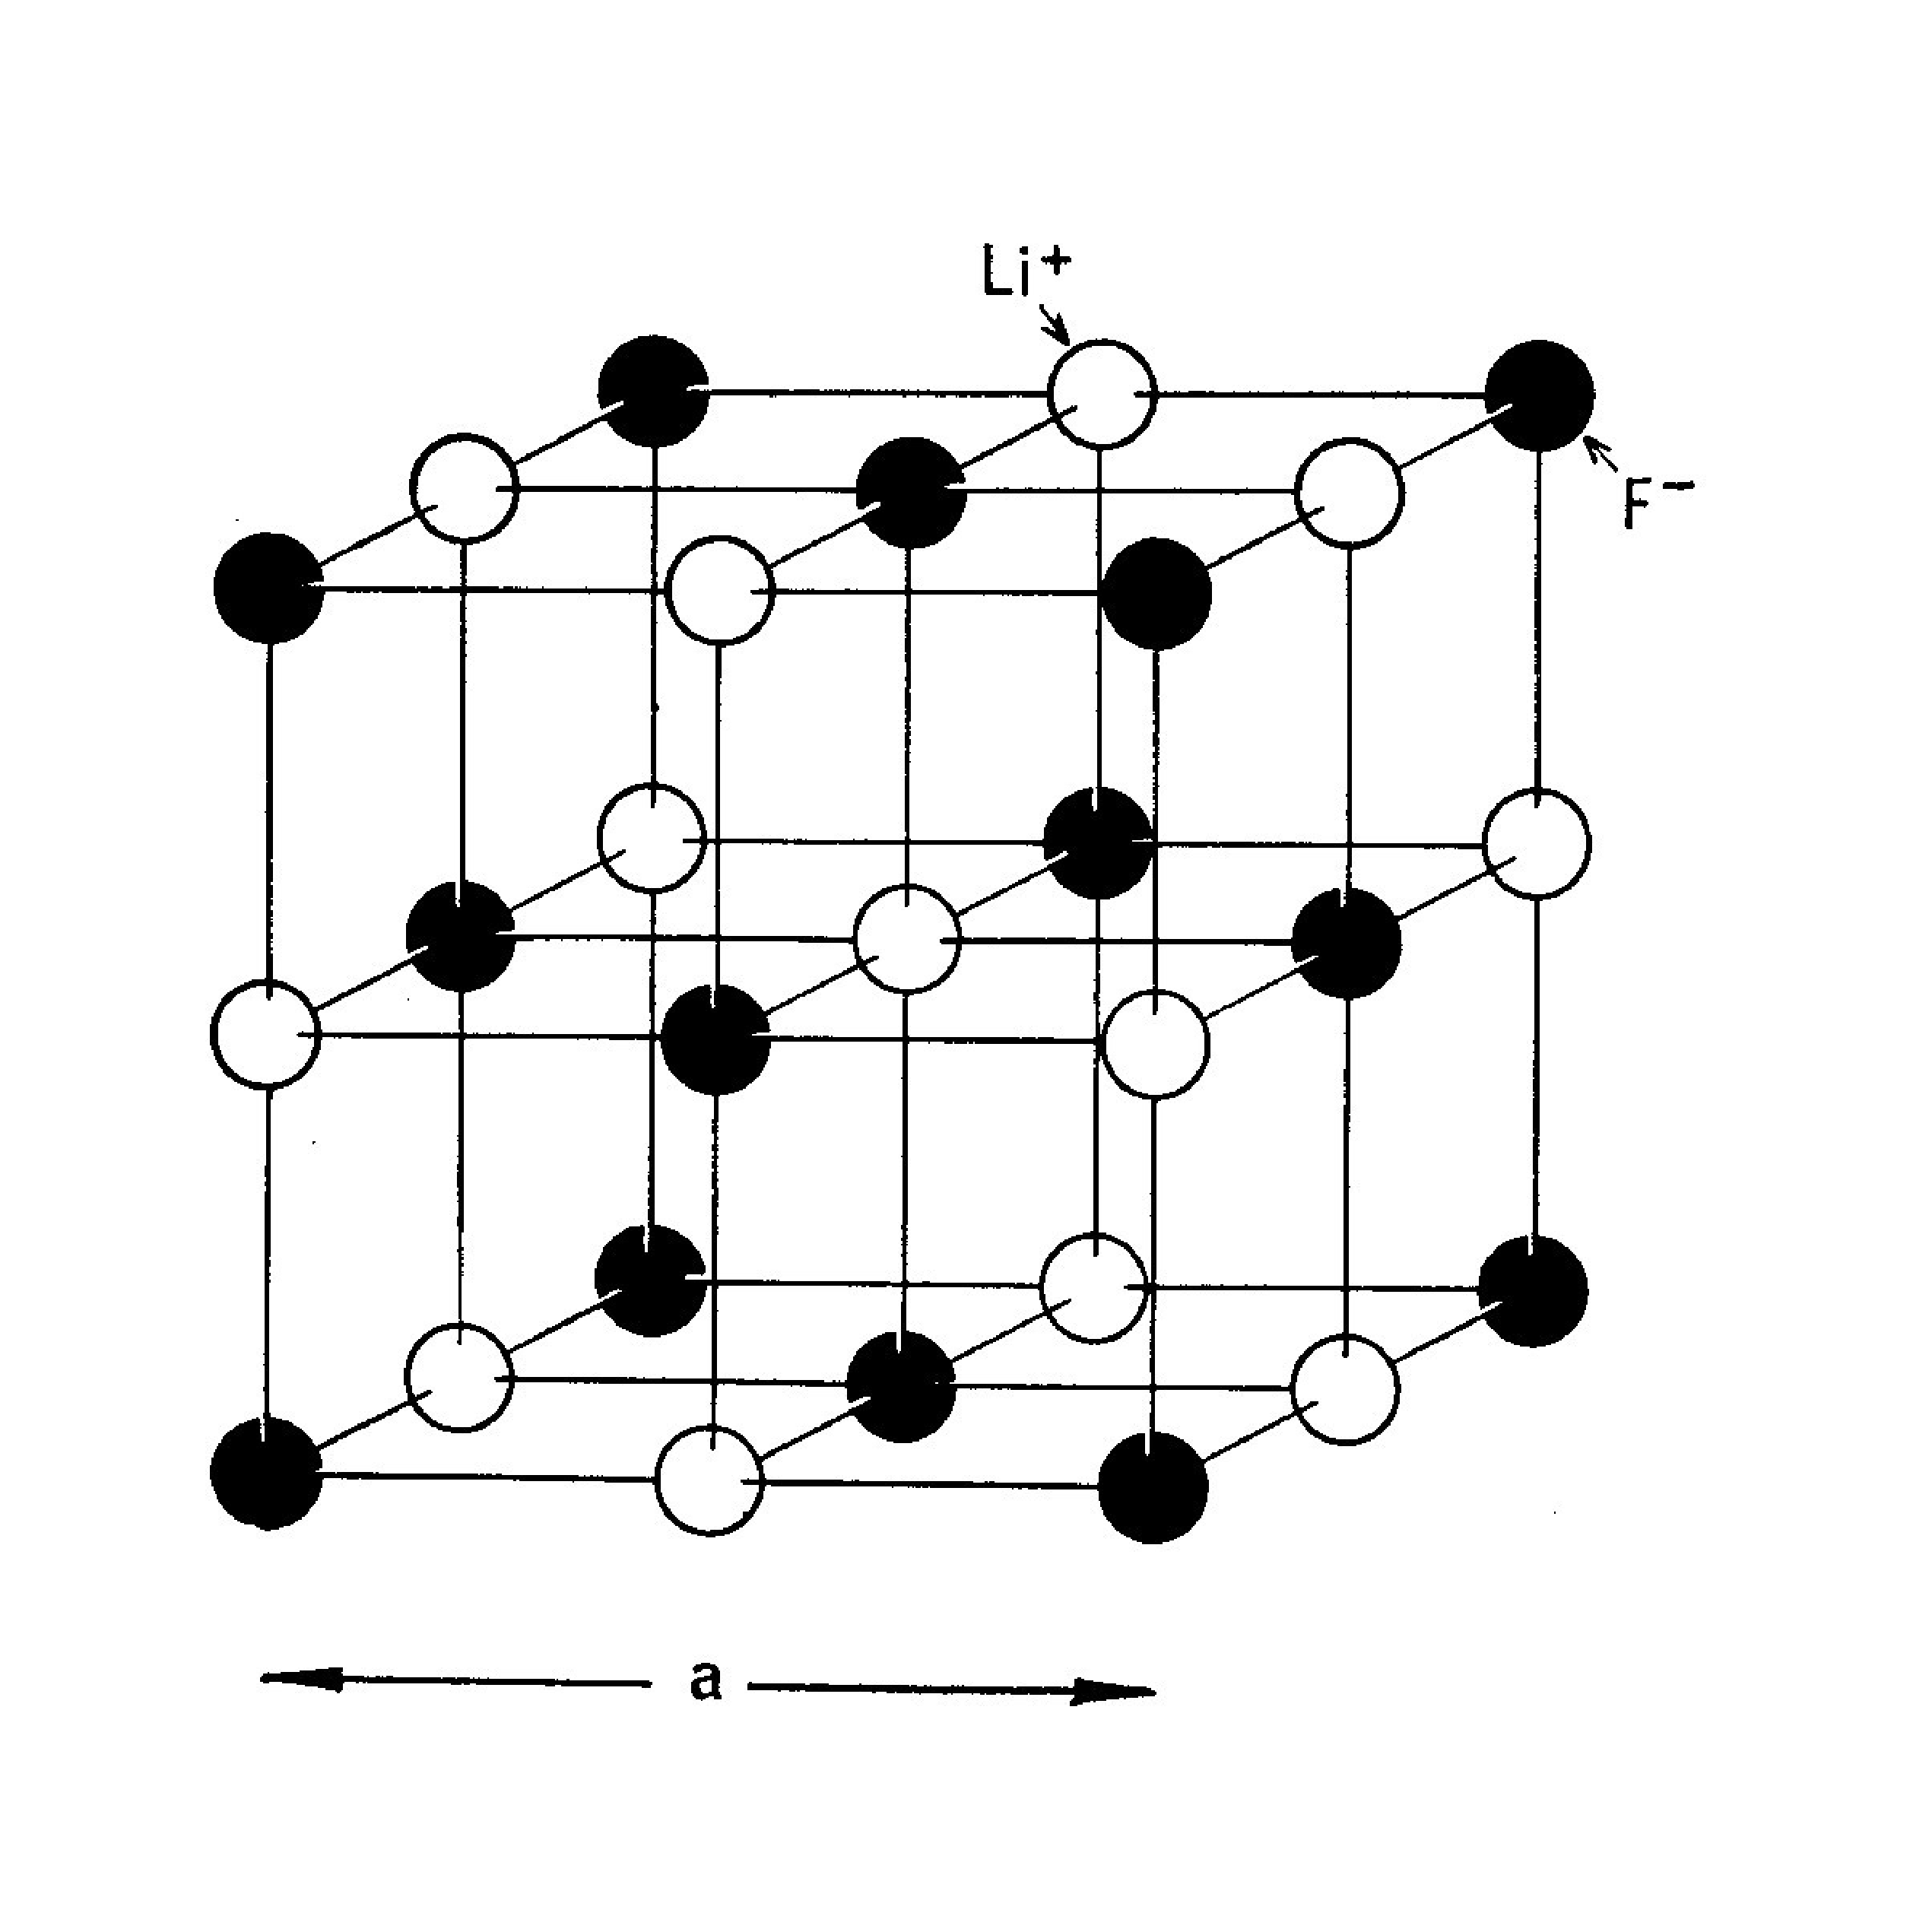
\includegraphics[width=0.5\textwidth]{../media/B2.8/LiF.pdf}
\caption{LiF Kristallgitter \cite[S. 9]{Newey}}
\label{abb:LiF Kristallgitter}
\end{figure}

\hypertarget{winkel-zwischen-den-kristalliten-einer-kleinwinkelkorngrenze}{%
\subsection{Winkel zwischen den Kristalliten einer
Kleinwinkelkorngrenze}\label{winkel-zwischen-den-kristalliten-einer-kleinwinkelkorngrenze}}

Für den Winkel $\theta$ zwischen den Kristalliten, die in einer
Korngrenze aufeinander treffen, lässt sich geometrisch folgender
Zusammenhang zum Abstand $d$ zweier Ätzgrübchen und dem Betrag $b$ des Burgers-Vektors finden.
\begin{eqnarray}
    \sin(\theta) &=& \frac{b}{d}
\end{eqnarray}

\noindent
Ist die Korngrenze eine Kleinwinkelkorngrenze ($\theta < 15^\circ$), so lässt sich die Kleinwinkelnäherung für den Sinus nutzen.
\begin{eqnarray}
    \sin(\theta) &\approx& \theta \\
    \Rightarrow \theta &\approx& \frac{b}{d}
\end{eqnarray}

\noindent
Der wahrscheinlichste Burgers-Vektor $\vec{b}$ für $\mathrm{LiF}$ ist wie beschrieben der Vektor $[\frac{1}{2}\,0\,\frac{1}{2}]$ mit einer Länge von $b = \frac{a}{\sqrt{2}}$.
\begin{eqnarray}
    \theta &\approx& \frac{a}{\sqrt{2} \cdot d} \\
        &=& \frac{0.402\,\mathrm{nm}}{\sqrt{2} d}\\
    \theta &\approx& \frac{0.284\,\mathrm{nm}}{d} \label{theta}
\end{eqnarray}

\hypertarget{gleitsysteme-bei-mechanischer-belastung}{%
\subsection{Gleitsysteme bei mechanischer
Belastung}\label{gleitsysteme-bei-mechanischer-belastung}}

Aufgrund der Empfindlichkeit des Materials erzeugt jede mechanische
Belastung Gitterfehler in einem Kristall. Bei einem Nadeleindruck werden
Gleitsysteme mit bestimmten Ebenen sowie Richtungen aktiviert, dabei
entsteht eine Rosettenform, siehe Abbildung \ref{abb:Rosette}. Die Gleitebenen sind dabei die $\lbrace1\,1\,0\rbrace$-Ebenen, was in Abbildung \ref{abb:Schema Rosette} dargestellt ist. Zusammen mit dem Gleitvektor in $\expval{1\,1\,0}$-Richtungen bilden sie bei Lithiumflourid insgesamt sechs Gleitsysteme.

Die Arme der Rosette bestehen aus Versetzungen und zwar sowohl Stufen-
als auch Schraubenversetzungen. In $\expval{1\,0\,0}$-Richtungen werden Schraubenversetzungen und in $\expval{1\,1\,0}$-Richtungen Stufenversetzungen produziert. Die Arme in $[1\,1\,0]$-Richtung sind,
wie in Abbildung \ref{abb:Schema Rosette} ersichtlich, länger und ausgeprägter, weil der Burgersvektor in dieser Richtung am kürzesten ist.

\begin{figure}[ht]
	\begin{minipage}[t]{.3\linewidth}
		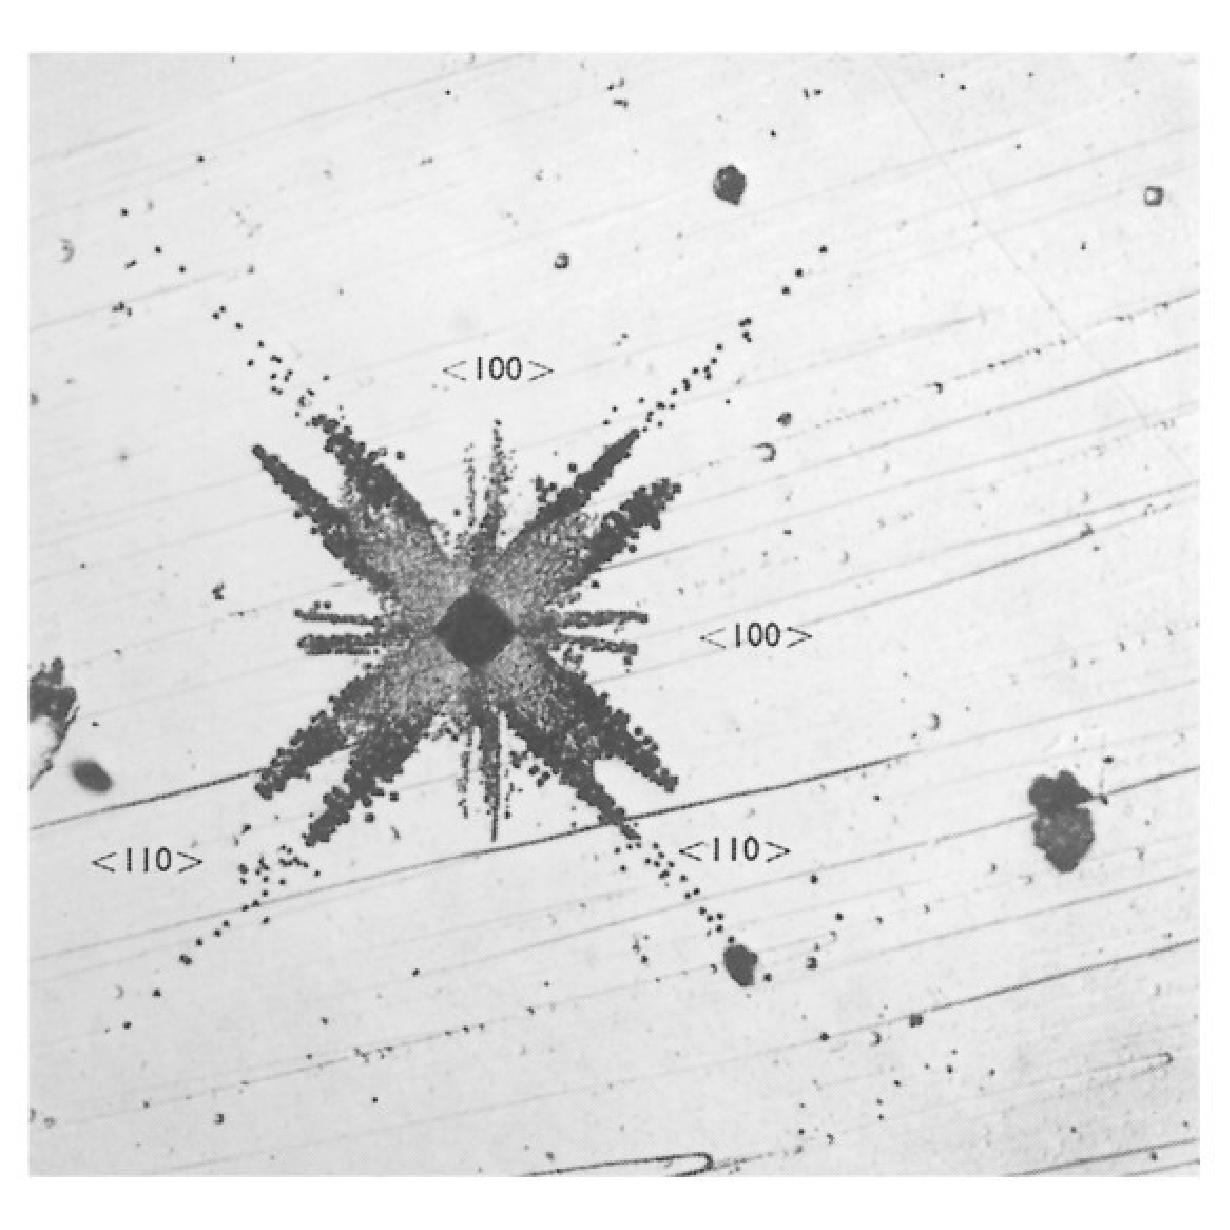
\includegraphics[width=\textwidth]{../media/B2.8/Nadeleindruck.pdf}
		\caption{Eine Rosette nach Nadeleindruck \cite[S. 18]{Newey}}
		\label{abb:Rosette}
	\end{minipage}
	\begin{minipage}[t]{.3\linewidth}
		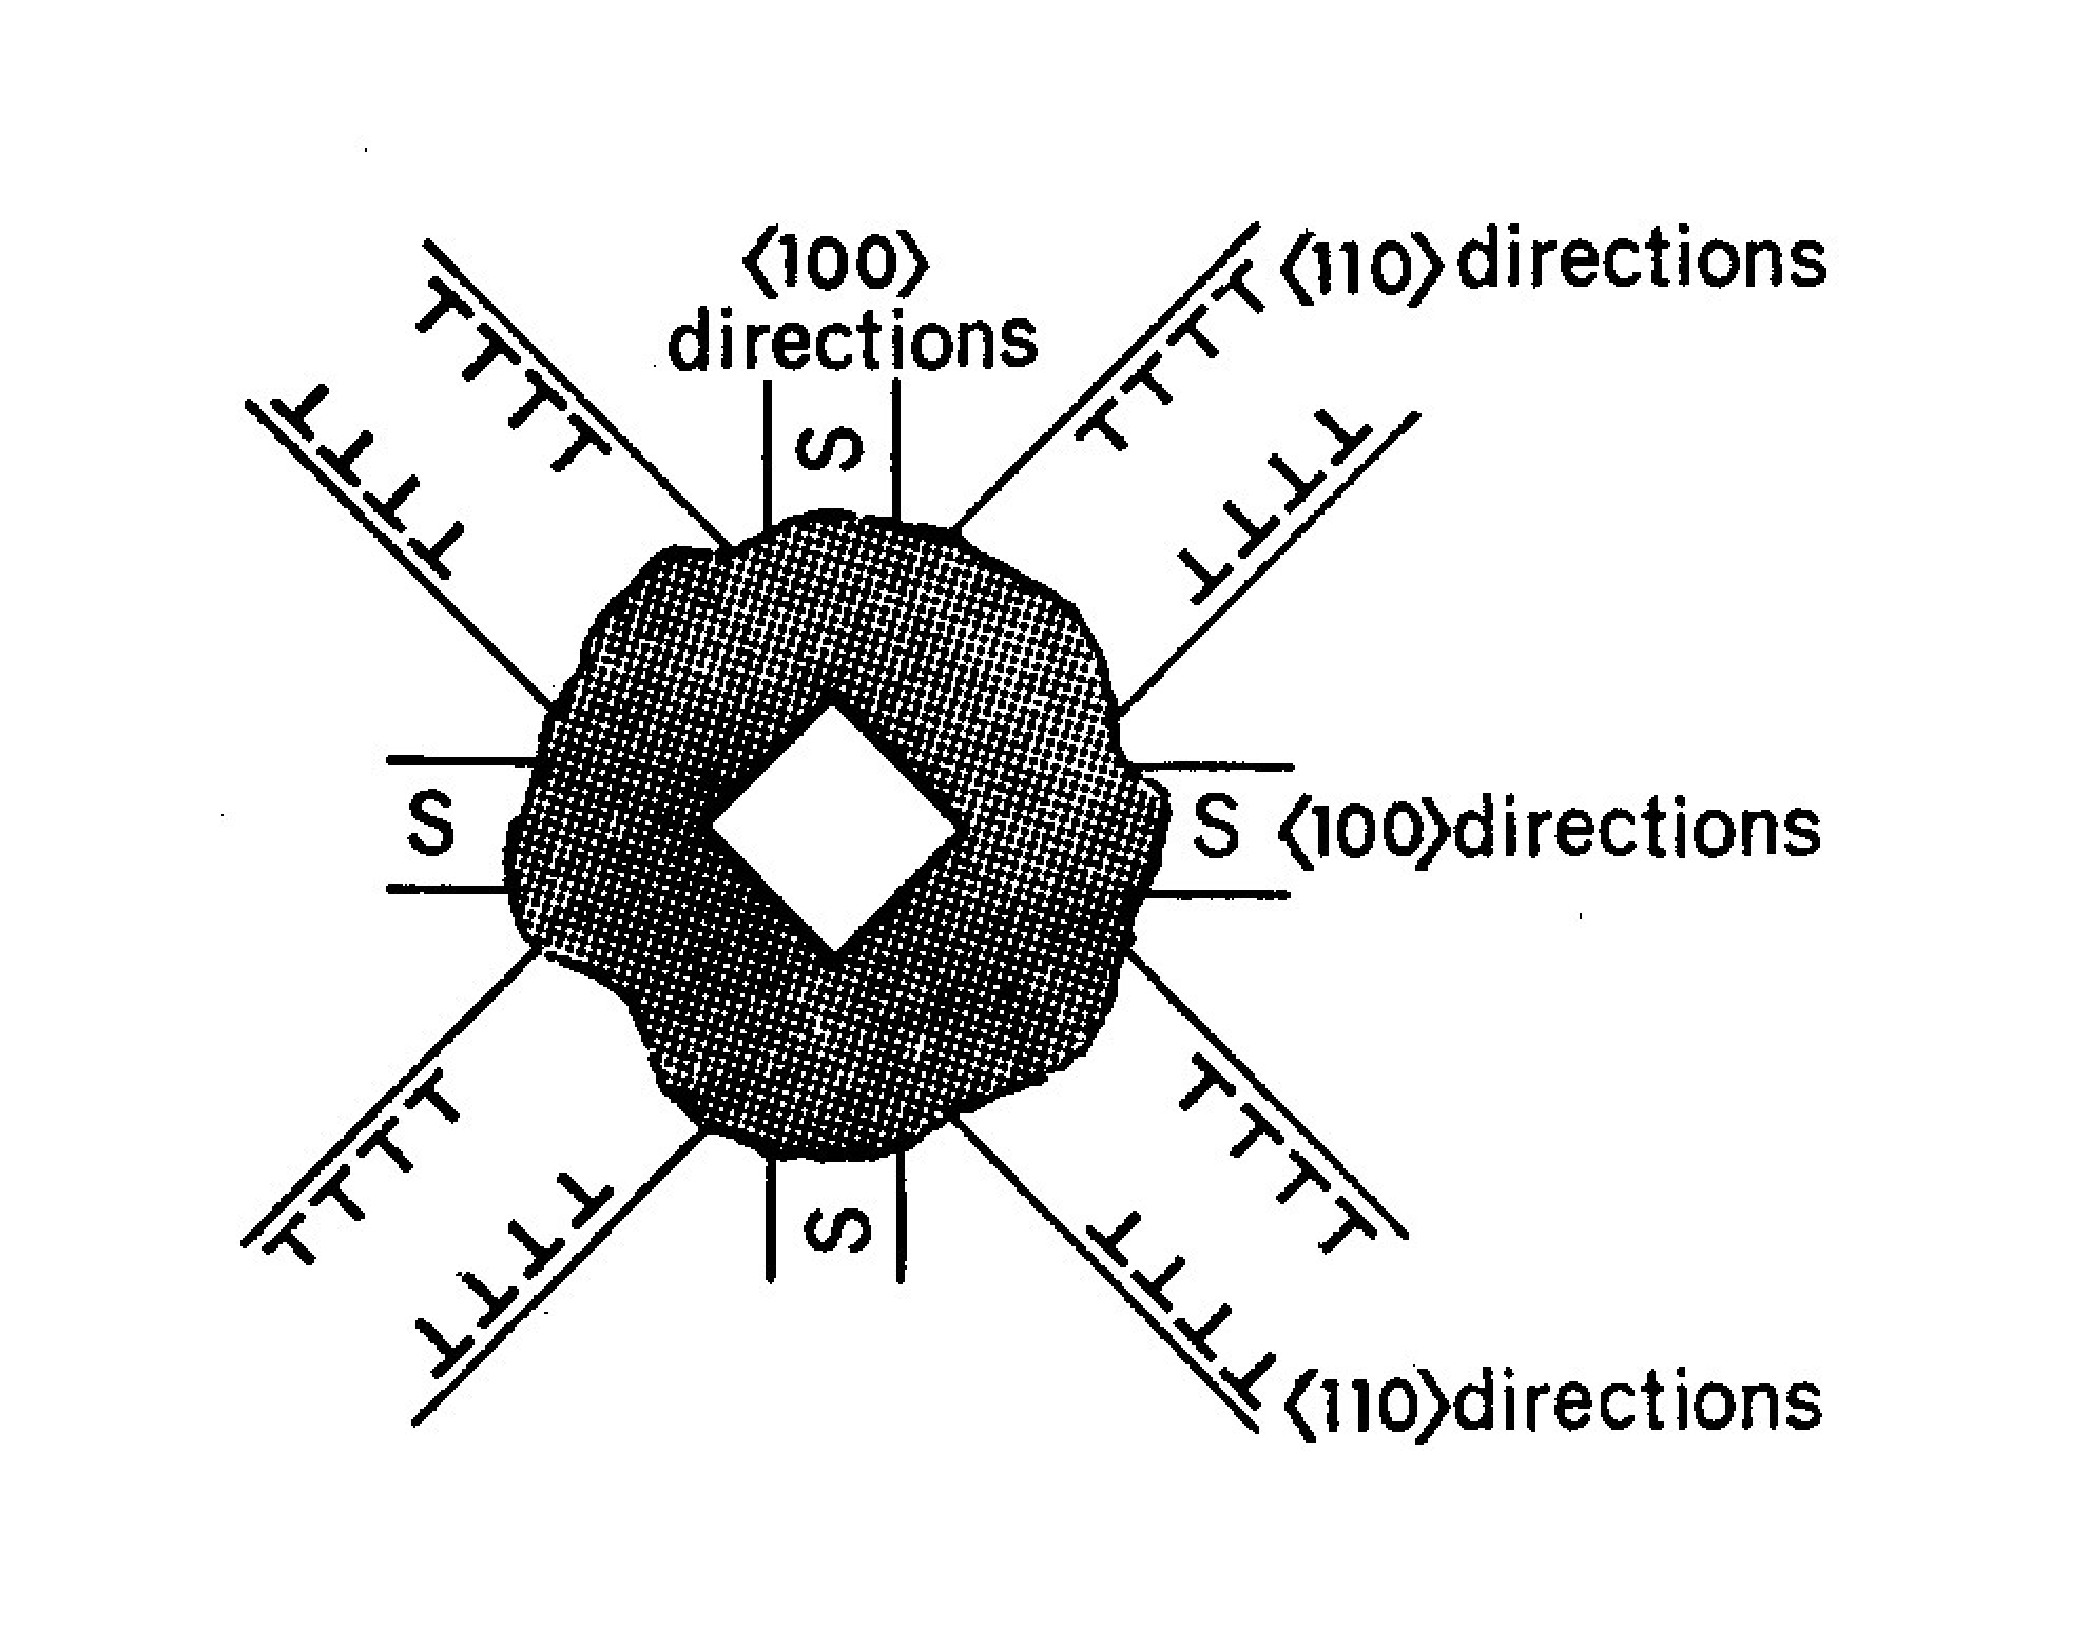
\includegraphics[width=\textwidth]{../media/B2.8/Rosette_Schema.pdf}
		\caption{Schematische Darstellung einer Rosette \cite[S. 21]{Newey}}
		\label{abb:Schema Rosette}
	\end{minipage}
	\begin{minipage}[t]{.3\linewidth}
		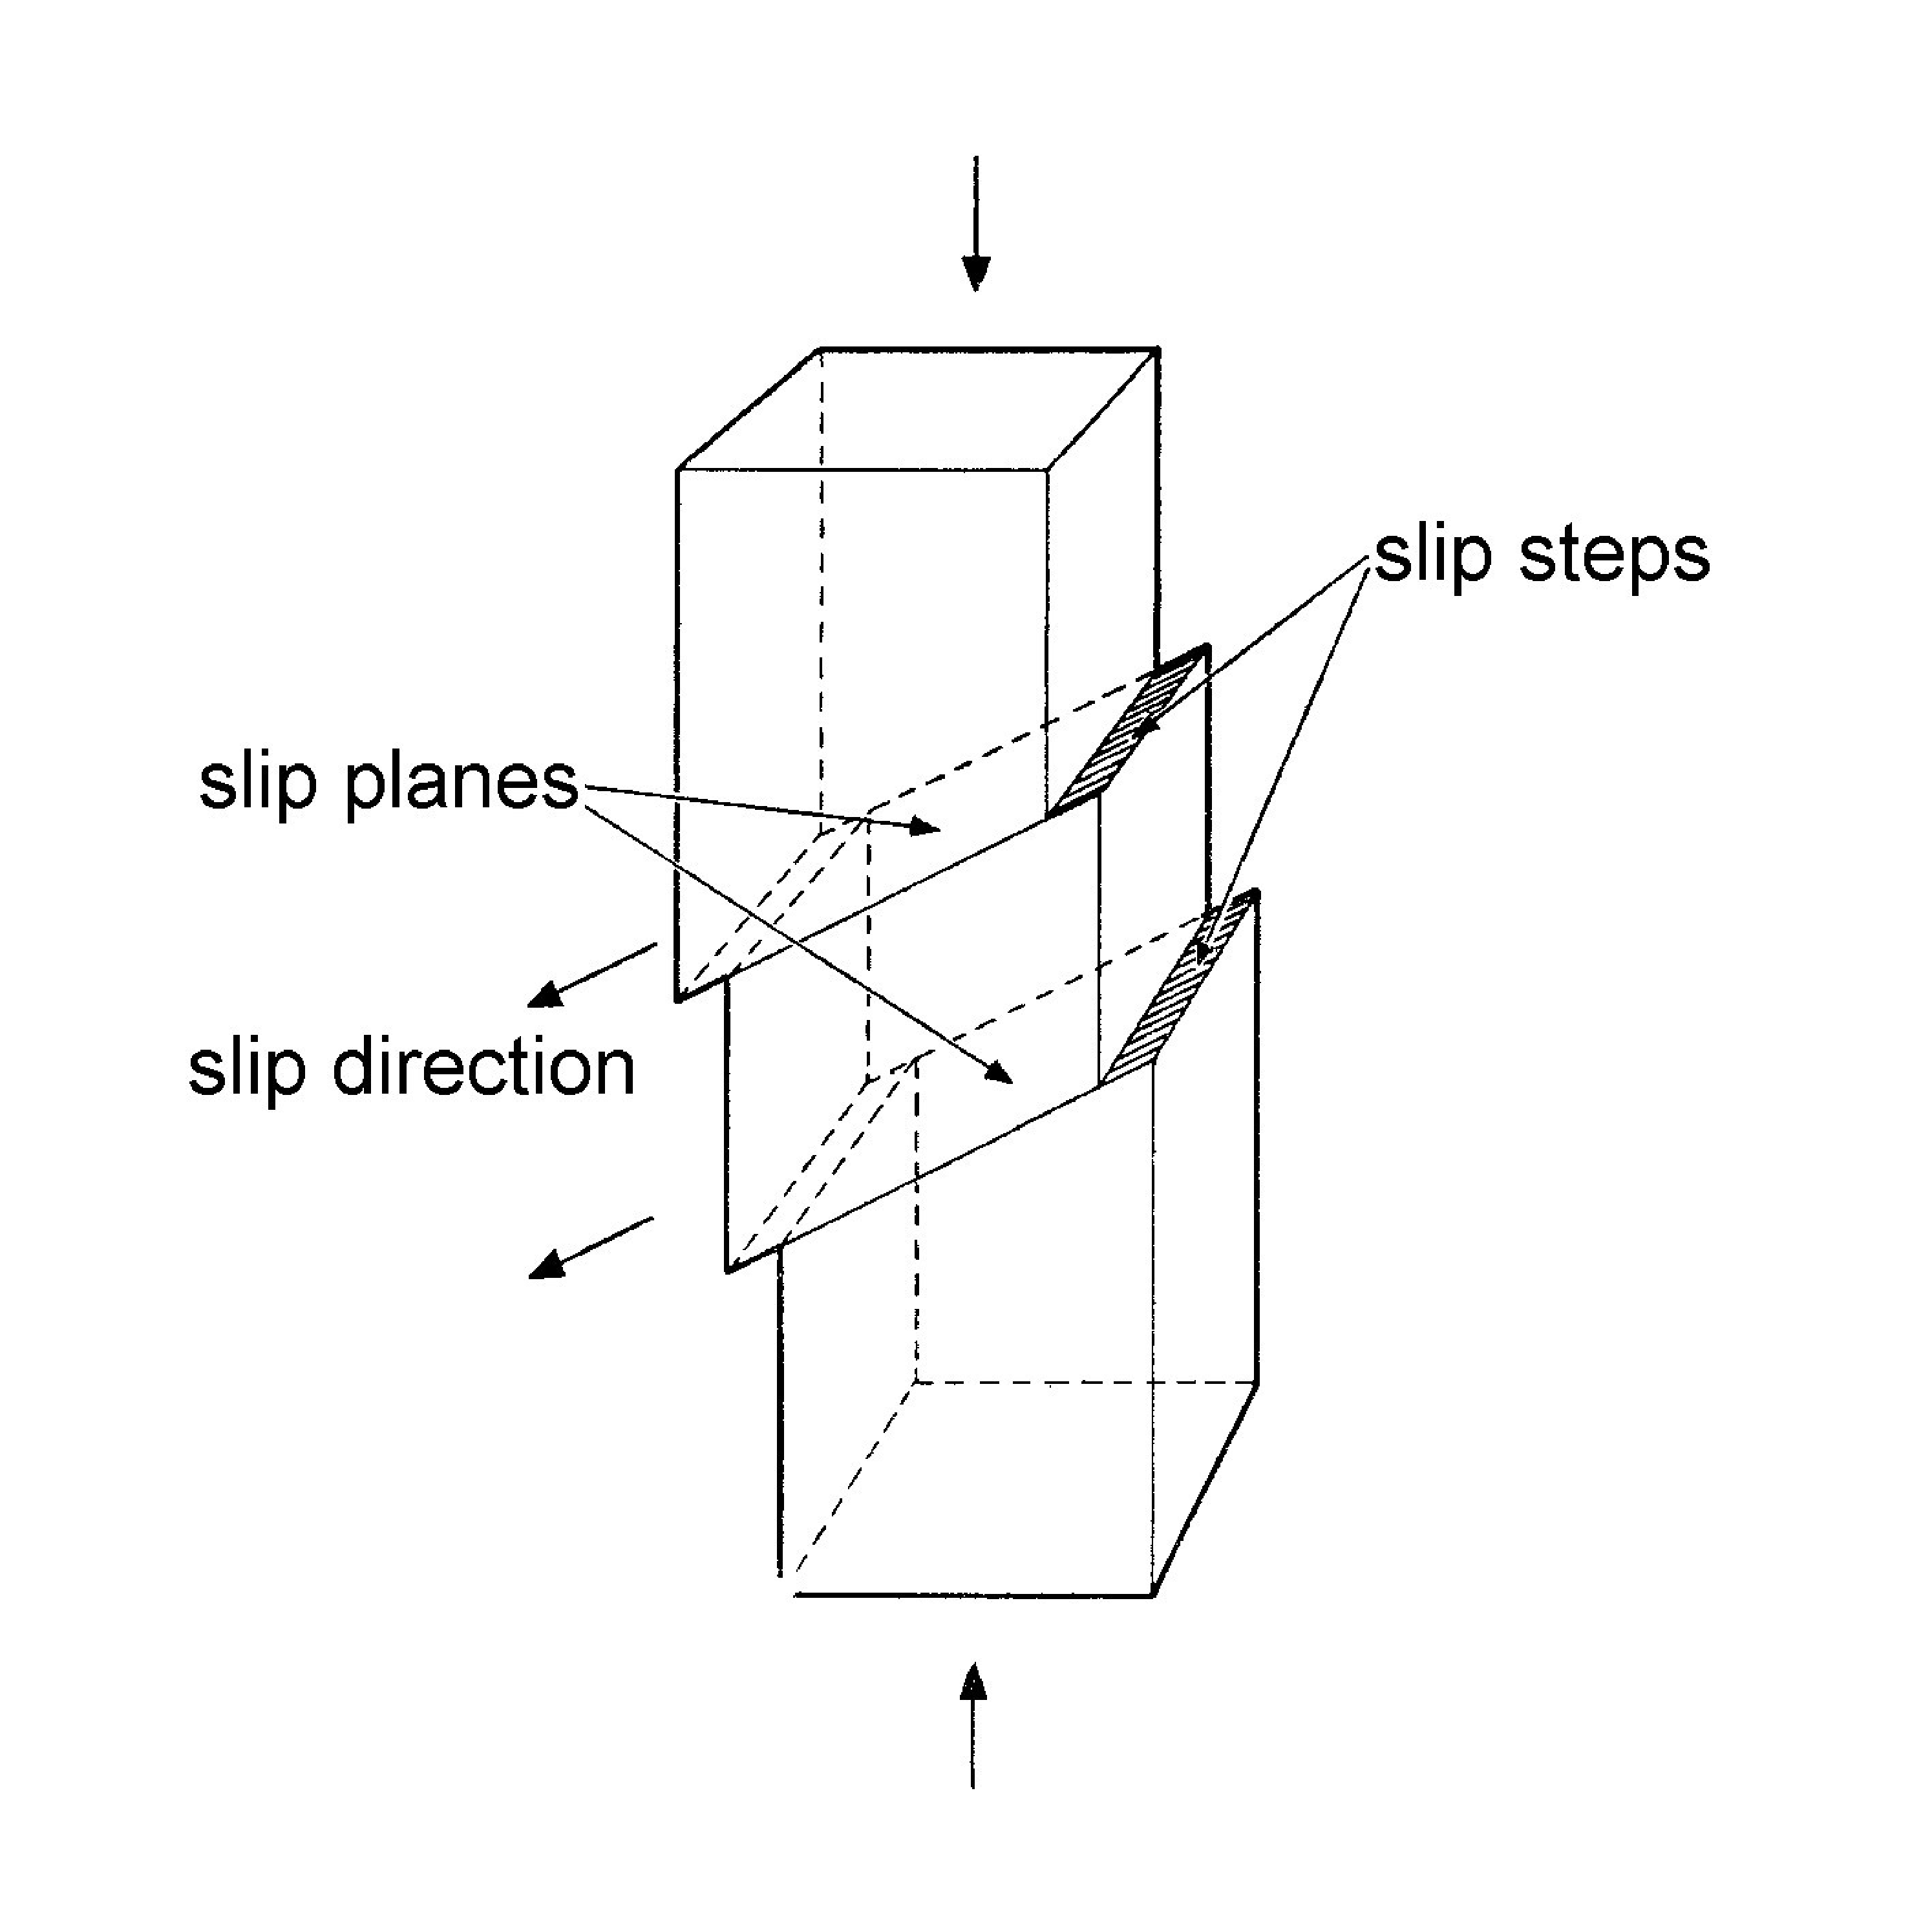
\includegraphics[width=\textwidth]{../media/B2.8/Gleitsysteme_Druck.pdf}
		\caption{Erwartetes Abgleiten unter Druck \cite[S. 2]{Newey}}
		\label{abb:Gleitebene}
	\end{minipage}

	\begin{minipage}[t]{\linewidth}
		\centering
		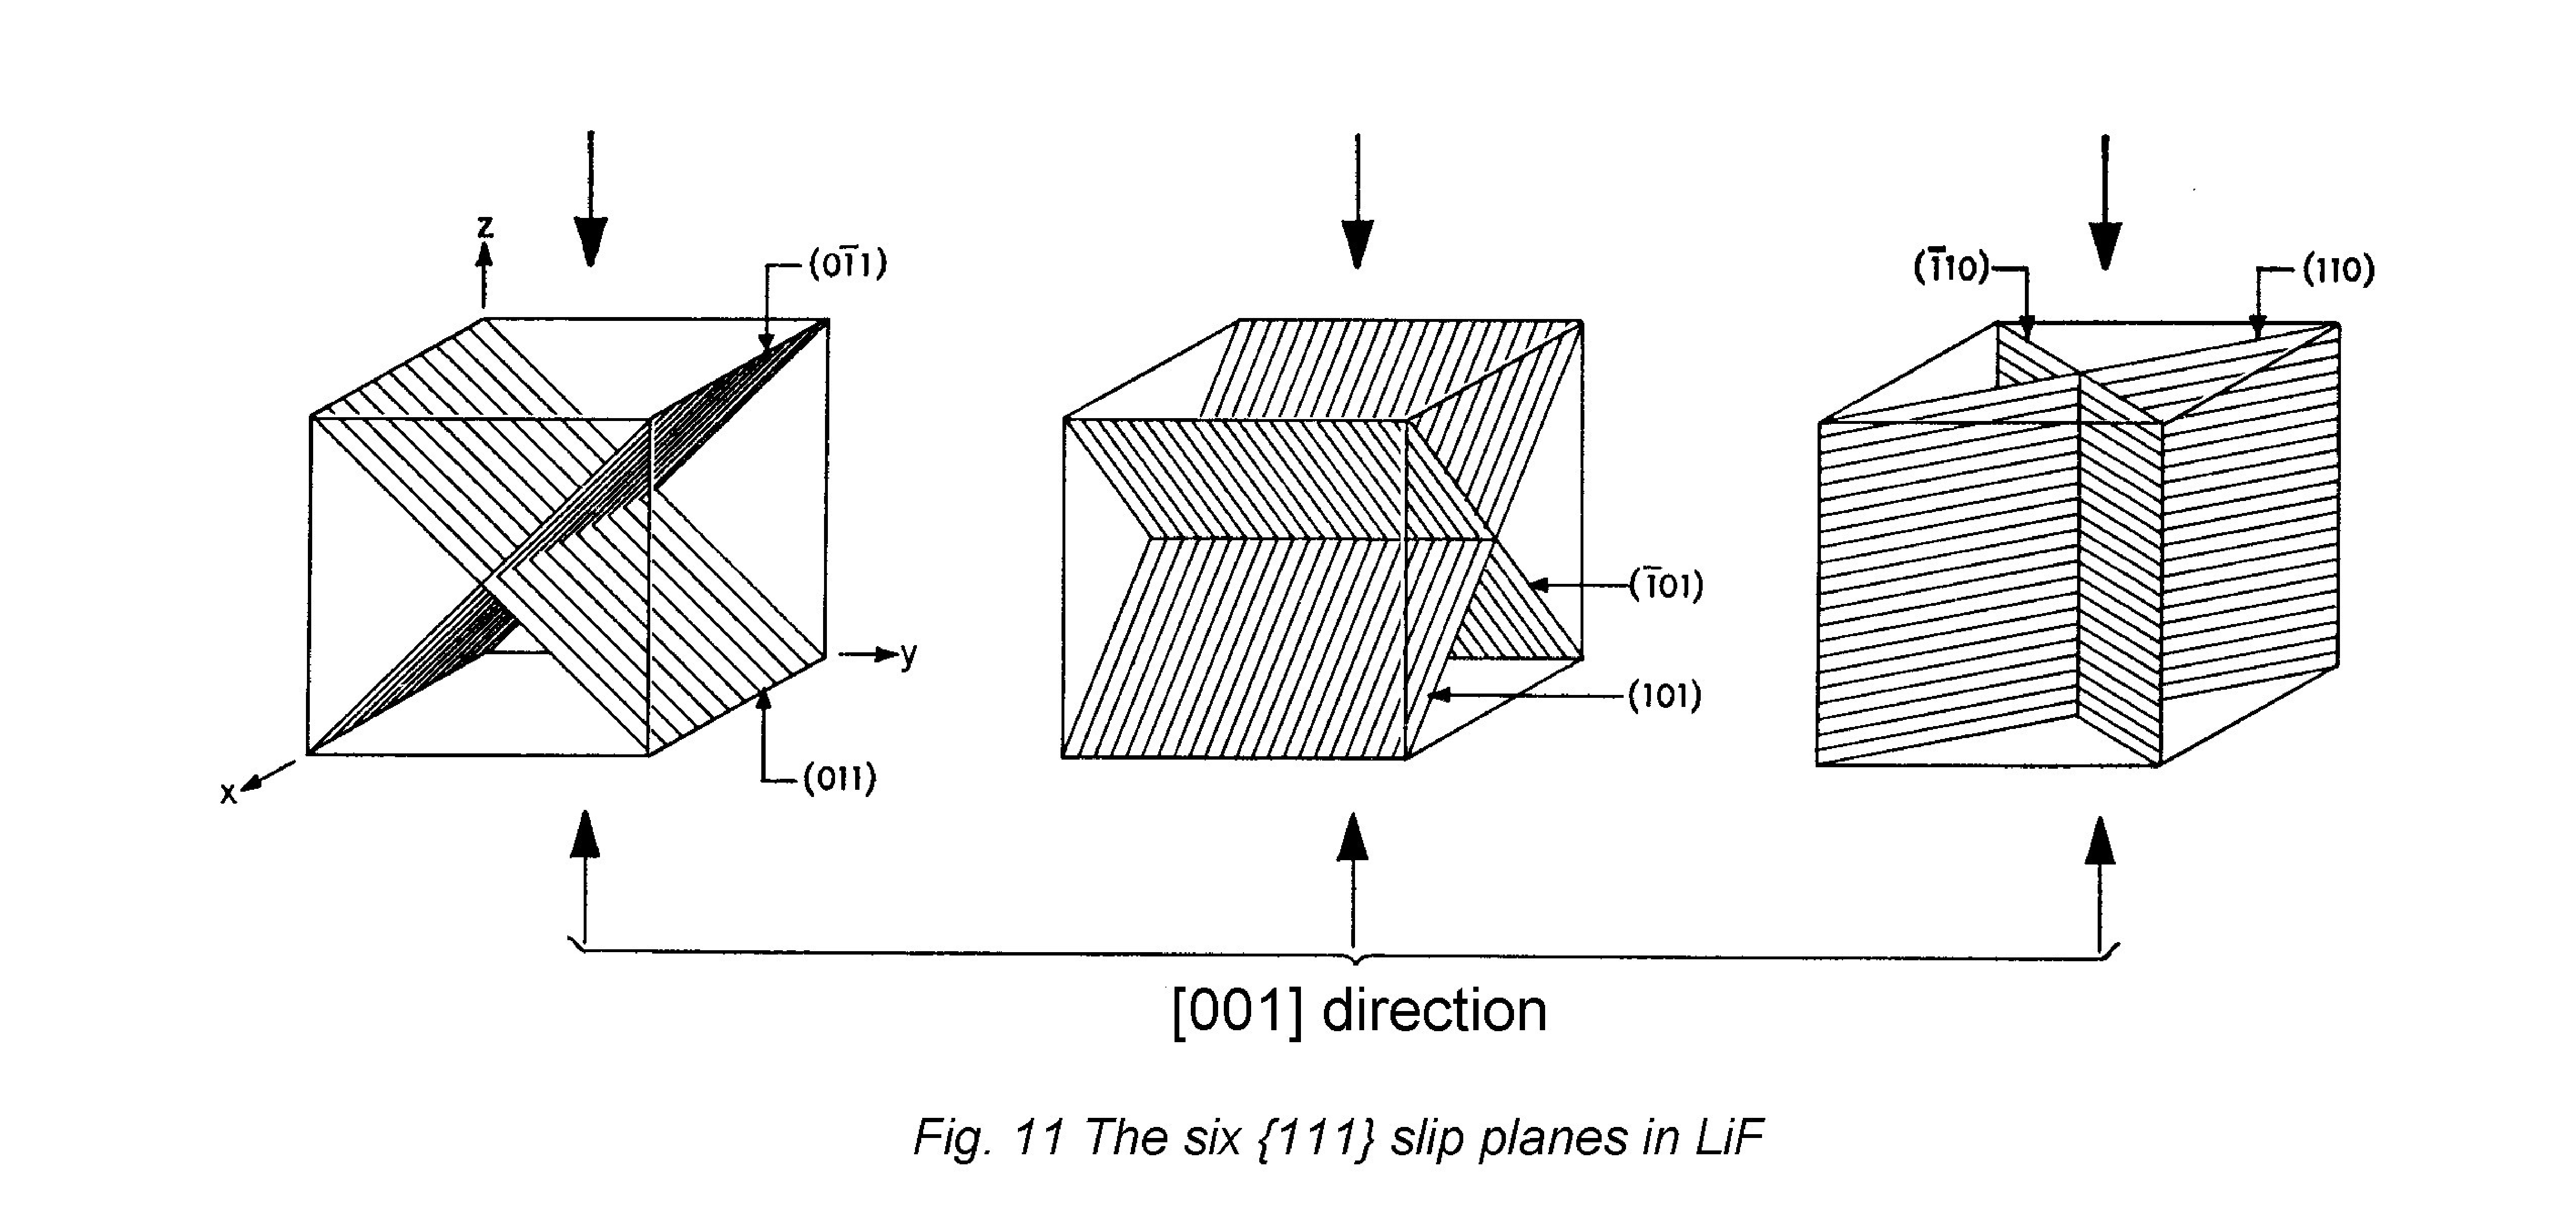
\includegraphics[width=0.9\linewidth]{../media/B2.8/Gleitsysteme.pdf}
		\caption{Gleitebenen in LiF \cite[S. 9]{Newey} }
		\label{abb:Gleitebenen LiF}
	\end{minipage}
\end{figure}

Wird die Probe axial unter Druck gesetzt, z.B. in der
$[0\,0\,1]$-Richtung, gibt es die vier potentiellen Gleitebenen
$(0\,\bar{1}\,1)$, $(0\,1\,1)$, $(\bar{1}\,0\,1)$ und
$(1\,0\,1)$, entlang derer Versetzungen laufen. Dies ist in Abbildung
\ref{abb:Gleitebenen LiF} ersichtlich.

Auf der $(\bar{1}\,1\,0)$-Ebene sowie der $(1\,1\,0)$-Ebene gibt es
keine Schubspannung, weil beide Ebenen parallel zur Hauptspannungsachse
liegen. Stattdessen ist ein Abgleiten in den $\lbrace1\,1\,0\rbrace$-Ebenen zu erwarten, was in Abbildung \ref{abb:Gleitebene} dargestellt ist. Ist der Druck auf die Probe bekannt, lässt sich die Schubspannung im Gleitsystem bestimmen.

\clearpage
\hypertarget{durchfuxfchrung}{%
\section{Durchführung}\label{durchfuxfchrung}}

\hypertarget{vorbereitung-der-proben}{%
\subsection{Vorbereitung der Proben}\label{vorbereitung-der-proben}}

Eine Probe $\mathrm{LiF}$-Kristall mit äußeren Abmessungen von etwa
$15 \times 3 \times 3 \,\mathrm{mm^3}$ wird zur Verfügung gestellt. Es
wurde zuvor von einem größeren Kristall durch Spalten abgetrennt und
dann für $48$ Stunden bei $650\,^\circ\mathrm C$ getempert und
langsam abgekühlt.

Eine zweite wird zu Beginn des Versuchs von einem größeren Block
abgespalten. Diese wird nicht getempert, allerdings chemisch poliert und
geätzt. Das Abspalten erfolgt mit einem Beitel, der parallel zu einer
Seitenfläche des großen Blocks angesetzt wird.

\hypertarget{polieren-und-uxe4tzen}$ aus
Tetrafluoroborsäure $(\mathrm{HBF_4})$, zu $30\,\mathrm{Vol\%}$ aus
Salpetersäure $(\mathrm{HNO_3})$ und zu $60\,\mathrm{Vol\%}$ aus
Wasser $(\mathrm{H_2O})$. Das Ätzmittel ist $50\,\mathrm{ppm}$
Eisen(III)-Chlorid $(\mathrm{FeCl_3})$ in destiliertem Wasser.

Beide Proben wurden für $19\mathrm{\,min}$ in das Poliermittel
gegeben. Nach $13.5\mathrm{\,min}$ wurden sie umgedreht, sodass alle
Seiten poliert wurden. Daraufhin wurden sie mit Ethanol abgespült,
jeweils $6.5\mathrm{\,min}$ geätzt und wiederum mit Ethanol abgespült.

\hypertarget{uxe4tzgruxfcbchendichten-kleinwinkelkorngrenzen}{%
\subsection{Ätzgrübchendichten \&
Kleinwinkelkorngrenzen}\label{uxe4tzgruxfcbchendichten-kleinwinkelkorngrenzen}}

Daraufhin wurden die Proben daraufhin untersucht, welche Seite die
wenigsten Schäden und Stufen hat. Diese Seite wurde jeweils für die
folgenden Messungen verwendet.

Dann wurden je Probe zwei Aufnahmen aufgenommen, auf denen
Ätzgrübchen erkennbar sind. Bei der getemperten Probe wurden je eine
Aufnahme bei $2000$-facher und bei $1000$-facher Vergrößerung
gemacht, bei der ungetemperten Probe je eine Aufnahme bei
$1000$-facher und $500$-facher Vergrößerung.

Dann wurden drei Kleinwinkelkorngrenzen auf der getemperten Probe
gesucht und bei $2000$-facher Vergrößerung vermessen. Hierzu wurden
jeweils $4$ bis $6$ Ätzgrübchen abgezählt.

\hypertarget{nadeldruckrosetten}{%
\subsection{Nadeldruckrosetten}\label{nadeldruckrosetten}}

Auf der getemperten Probe wurden an drei möglichst defektfreien Stellen
Eindrücke mit einer Nadel gemacht. Daraufhin wurde die Probe erneut für
$6\mathrm{\,min}$ geätzt und danach mit Ethanol abgespült.

Die dabei entstandenen Rosetten wurden fotografiert. Dazu wurde zunächst
eine Übersicht bei $50$-facher Vergrößerung aufgenommen und dann
Einzelaufnahmen bei $200$- bzw. $150$-fachen Vergrößerungen
aufgenommen. Hierbei fiel direkt auf, dass die Rosette im Zentrum der
Probe größere Ausmaße hatte, weswegen eine geringere Vergrößerung als
für die anderen beiden Rosetten notwendig war, um die gesamte Rosette
abzubilden.

\hypertarget{eingespannte-probe}{%
\subsection{Eingespannte Probe}\label{eingespannte-probe}}

Nun wurde die Probe hochkant so in eine Presse eingespannt, dass die
vermessene Seite senkrecht war. Die Spannung wurde durch ein
Gesamtgewicht von $1.789\mathrm{\,kg}$ erzeugt, das durch die obere
Hälfte der Presse und ein Zusatzgewicht von $841\mathrm{\,g}$ erzeugt
wurde.

Nach $2\mathrm{\,min}$ wurde die Probe herausgeholt und erneut für
$6\mathrm{\,min}$ geätzt. Nach erneuten Abspülen mit Ethanol wurden
die Rosetten erneut fotografiert. Hierbei wurde darauf geachtet, dass
sowohl alte Ätzgrübchen als auch durch Wandern neu entstandene
Ätzgrübchen auf den Fotos sichtbar waren. Dies lässt sich durch die
Größe und Form der Ätzgrübchen unterscheiden.

Zuletzt wurde eingespannte Fläche vermessen. Dazu wurde die Probe
senkrecht auf das Mikroskop gestellt, sodass die Orientierung der Probe
der Orientierung beim Einspannen entsprach. Mithilfe des Mikroskops
wurde die Oberfläche der Probenschmalseite vermessen.

\hypertarget{auswertung}{%
\section{Auswertung}\label{auswertung}}

\hypertarget{uxe4tzgruxfcbchendichte}{%
\subsection{Ätzgrübchendichte}\label{uxe4tzgruxfcbchendichte}}

\hypertarget{berechnung}{%
\paragraph*{Berechnung}\label{berechnung}}

Die Ätzgrübchendichte ist an verschiedene Stellen der jeweiligen Proben
sehr unterschiedlich, da durch die Ätzgrübchendichte lokale Unebenheiten
dargestellt werden.

Um die insgesamte Ätzgrübchendichte der beiden Proben abzuschätzen,
wurden für jede Probe an zwei repräsentativen Stellen Ätzgrübchen
aufgenommen, wobei die Ätzgrübchendichte $N$ durch die Anzahl $n$
der Ätzgrübchen und die Fläche $F$ bestimmt ist. Die Ungenauigkeit
$\Delta N$ der Ätzgrübchendichte ist nach Gauß'scher
Fehlerfortpflanzung zu bestimmen.
\begin{eqnarray}
    N &=& \frac{n}{F} \label{N}\\
    \Delta N &=& \sqrt{
        \left(\frac{\Delta n}{F}\right)^2
        + \left(\frac{n}{F^2} \cdot \Delta F\right)^2} \label{DeltaN}
\end{eqnarray}

Der Fehler der Anzahl der Ätzgrübchendichte $\Delta n$ hängt neben
menschlicher Ablesefähigkeit auch von der Schärfe des jeweiligen Bildes
ab. Wir schätzen ihn dennoch für alle Bilder auf $10\,\%$, da in
unserem Fall die Bilder mit höherer Unschärfe auch die kleinere Anzahl
an Ätzgrübchen haben. Der Fehler der Fläche $\Delta F$ ist durch die
Genauigkeit der Streckenangabe des Mikroskops gegeben und beträgt
$\Delta F=(0.005 \mathrm{\, \mu m})^2$.

Um die durchschnittliche Ätzgrübchendichte der Proben zu bestimmen,
wird der Mittelwert der Dichten an den zwei Stellen ermittelt, die
Ungenauigkeit ist durch die Standardabweichung gegeben.
\begin{eqnarray}
    \bar{N} &=& \frac{N_1 + N_2}{2} \label{Nbar}\\
    \Delta \bar N &=& \left| \frac{N_1 - N_2}{2} \right| \label{DeltaNbar}
\end{eqnarray}

\hypertarget{nicht-getemperte-probe}{%
\paragraph*{Nicht-getemperte Probe}\label{nicht-getemperte-probe}}

Wie in Abbildung \ref{abb:dichte_nt_1} zu sehen, sind in den inneren sechs blauen Quadraten insgesamt $5\pm1$ Ätzgrübchen zu finden, die Quadrate haben
jeweils eine Seitenlänge von $200.00 \mathrm{\,\mu m}$.

An der zweiten Stelle der nicht getemperten Probe (siehe Abbildung
\ref{abb:dichte_nt_2}) sind in den inneren sechs blauen Quadraten $16\pm1$
Ätzgrübchen zu finden, die Quadrate hier je eine Seitenlänge von
$100.00 \mathrm{\, \mu m}$.

\begin{figure}[ht]
	\begin{minipage}[t]{.5\linewidth}
		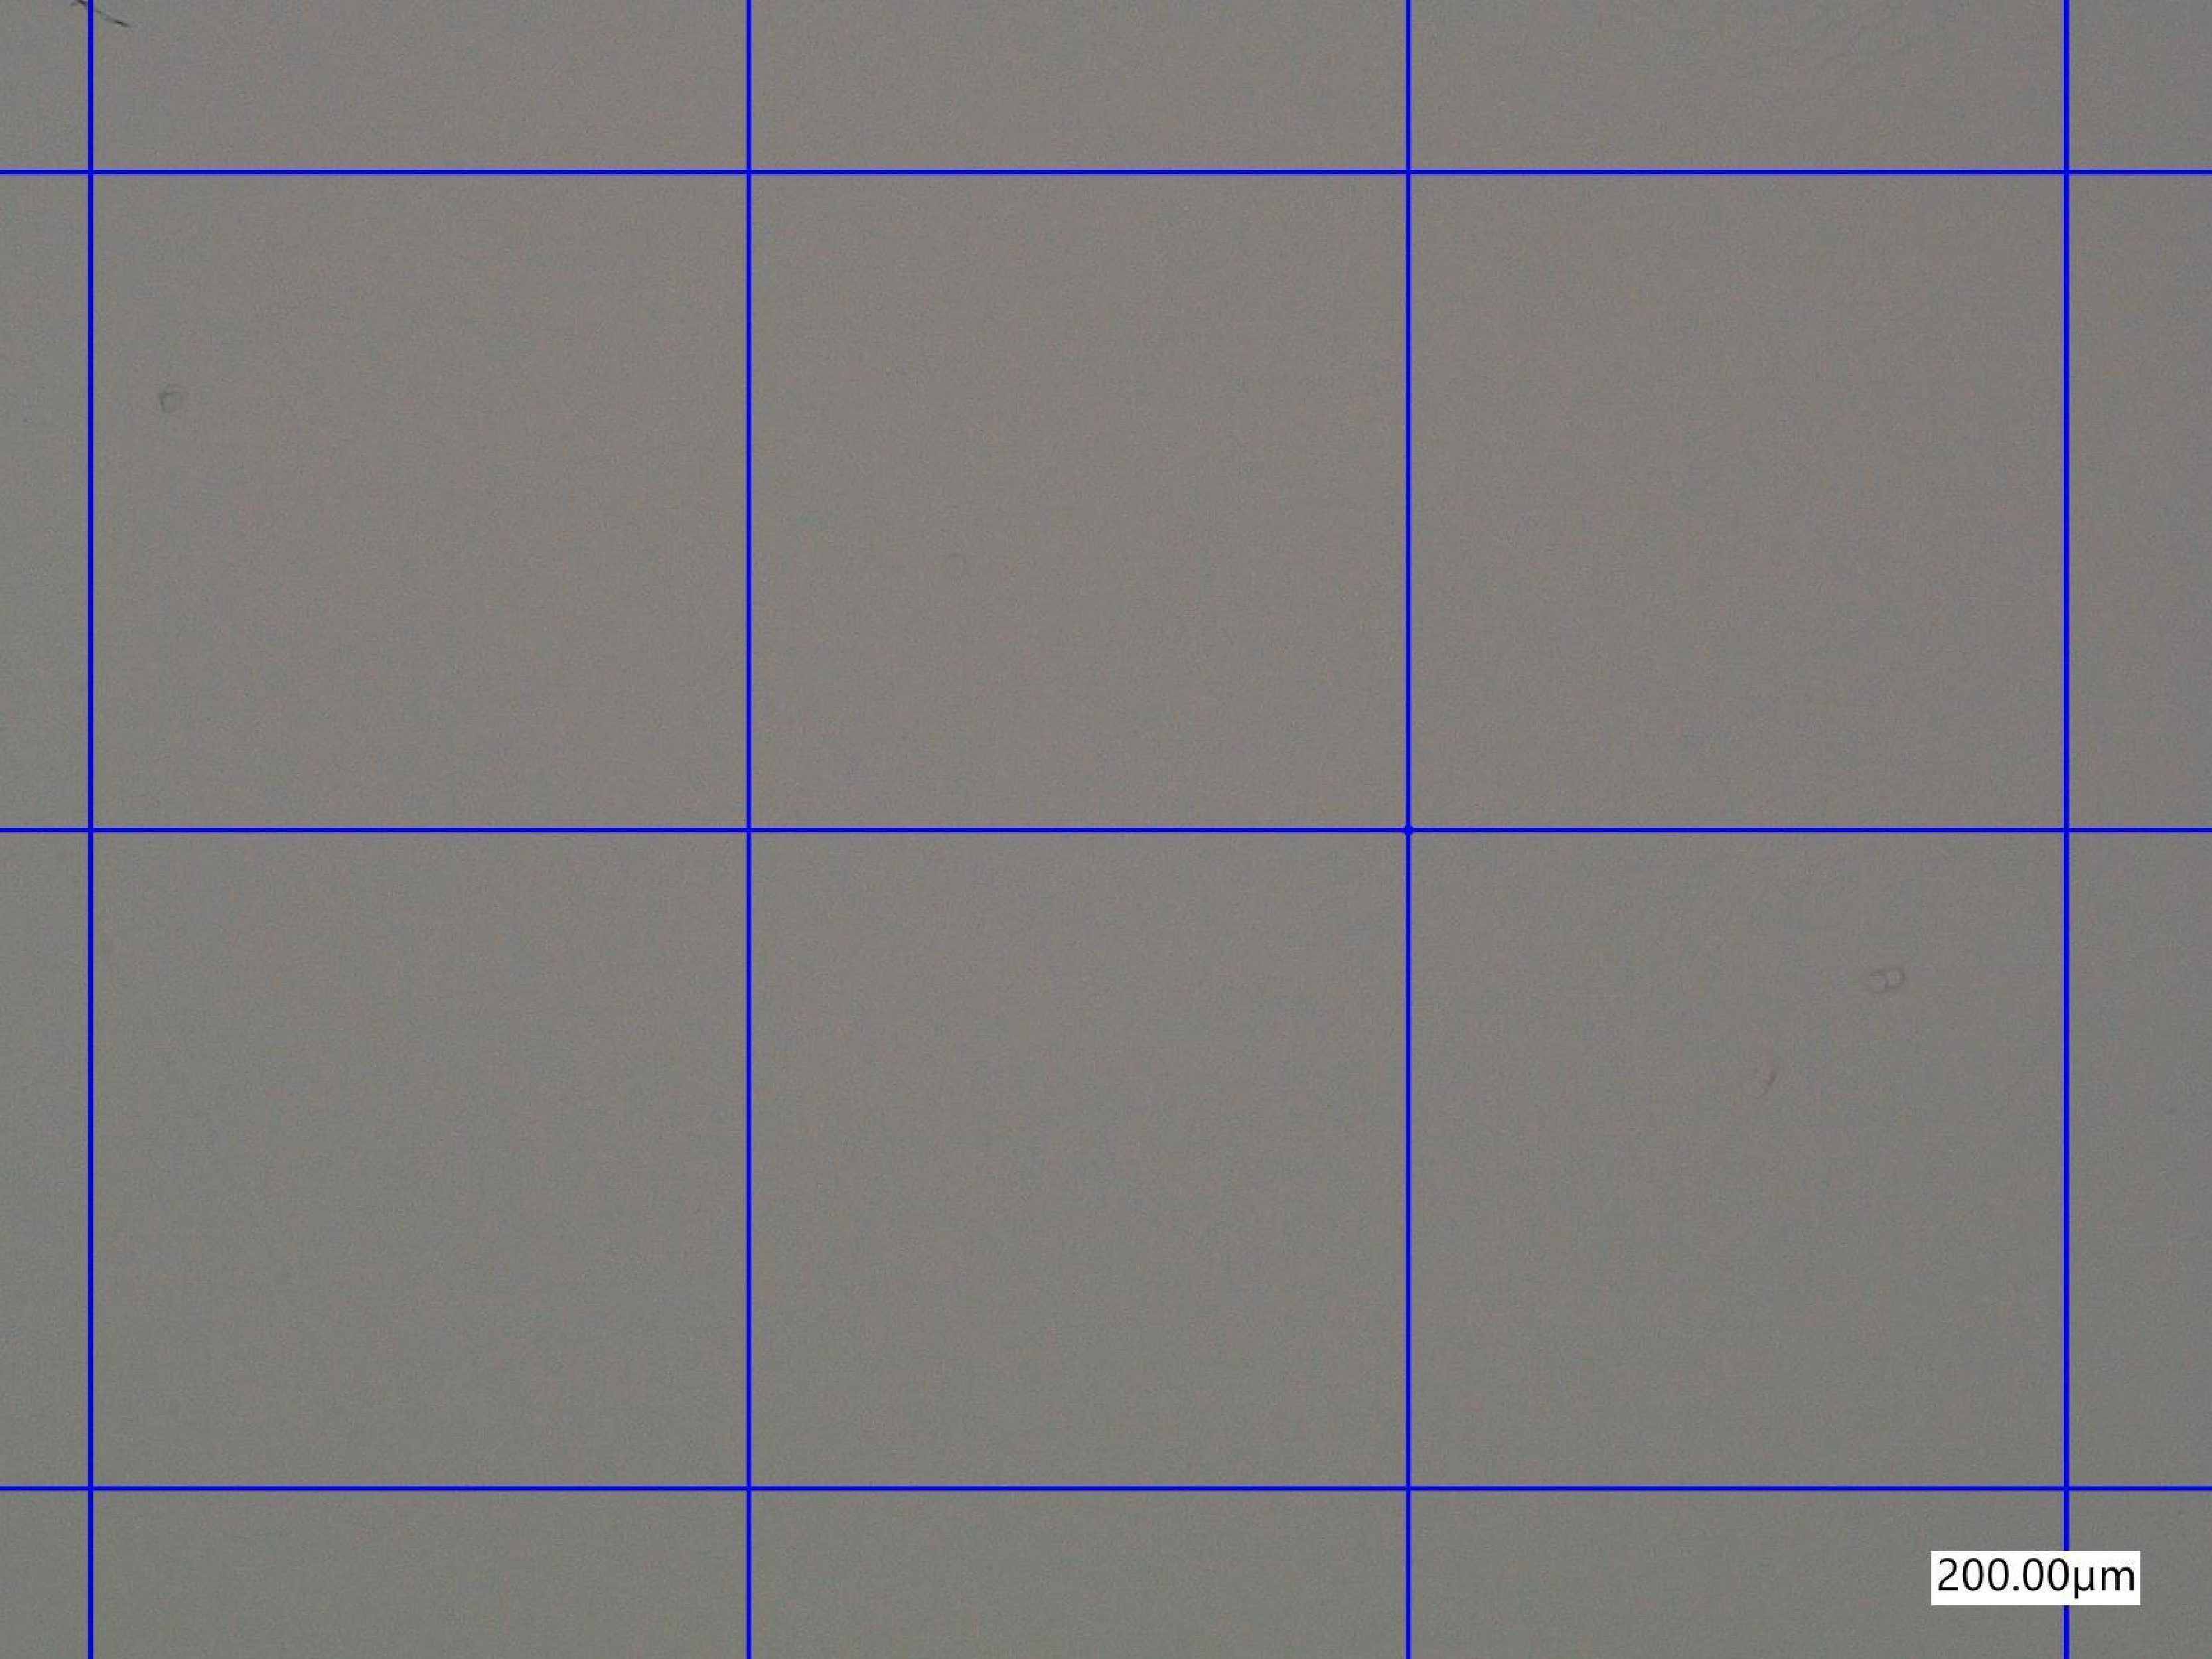
\includegraphics[width=\textwidth]{../media/B2.8/Dichte1_not_tempered.pdf}
		\caption{Ätzgrübchendichte nicht-getemperte Probe, Aufnahme $1$}
		\label{abb:dichte_nt_1}
	\end{minipage}
	\begin{minipage}[t]{.5\linewidth}
		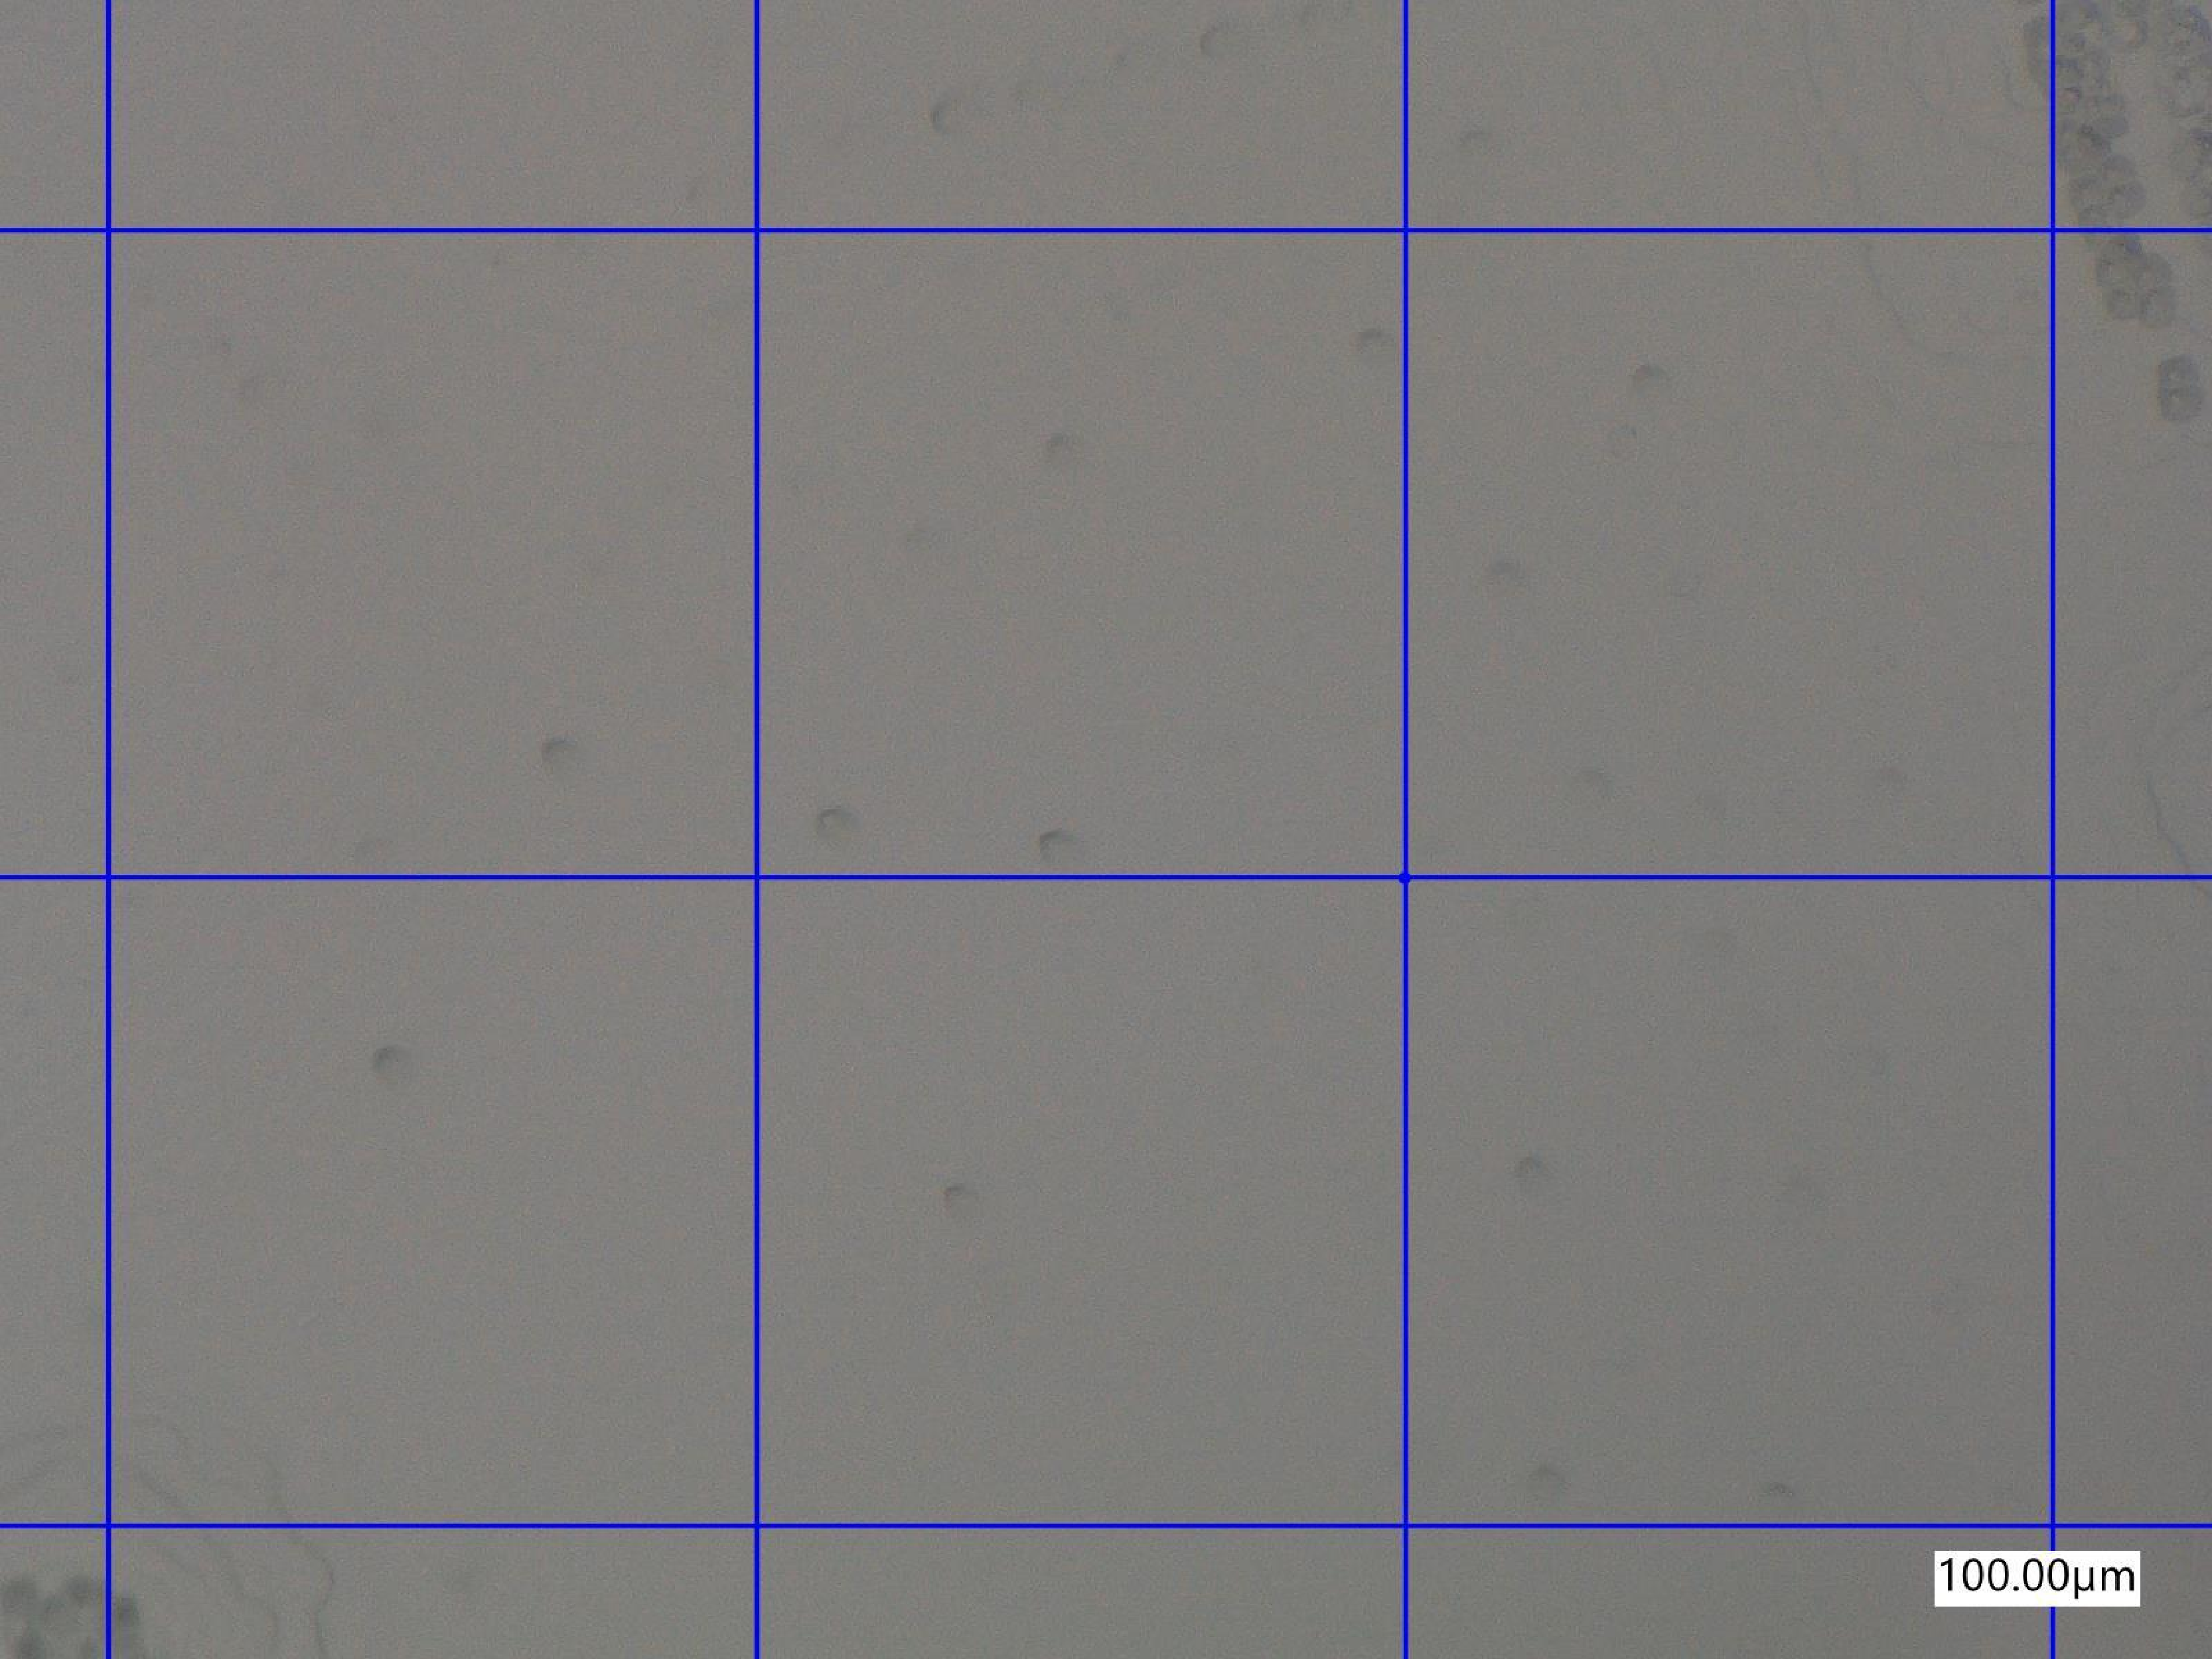
\includegraphics[width=\textwidth]{../media/B2.8/Dichte2_not_tempered.pdf}
		\caption{Ätzgrübchendichte nicht-getemperte Probe, Aufnahme $2$}
		\label{abb:dichte_nt_2}
	\end{minipage}
\end{figure}

Mithilfe der Gleichungen $\eqref{N}$ bis $\eqref{DeltaNbar}$ folgt
die mittlere Ätzgrübchendichte $\bar N_\mathrm{nt}$ der
nicht-getemperten Probe.
\begin{eqnarray}
    N_\mathrm{nt,1} &=& (2.1 \pm 0.4) \cdot 10^3 \mathrm{\, cm^{-2}} \\
    N_\mathrm{nt,2} &=& (2.7 \pm 0.3) \cdot 10^{4} \mathrm{\, cm^{-2}} \\
    \bar N_\mathrm{nt}
        &=& (1.4 \pm 1.2) \cdot 10^4 \mathrm{\, cm^{-2}}
        \quad(\pm 85.52\,\%)
\end{eqnarray}

\hypertarget{getemperte-probe}{%
\paragraph*{getemperte Probe}\label{getemperte-probe}}

In Abbildung \ref{abb:dichte_t_1} sind insgesamt $50$ Ätzgrübchen in den inneren
acht blauen Quadraten zu entdecken. Jedes dieser Quadrate hat eine
Seitenlänge von $150.00 \mathrm{\, \mu m}$.

Die zweite Stelle der getemperten Probe ist in Abbildung \ref{abb:dichte_t_2} zu
sehen. Dort sind $81\pm8$ Ätzgrübchen in den inneren zwölf blauen
Quadraten zu finden. Jedes der Quadrate hat eine Seitenlänge von
$70.00 \mathrm{\, \mu m}$.

\begin{figure}[ht]
	\begin{minipage}[t]{.5\linewidth}
		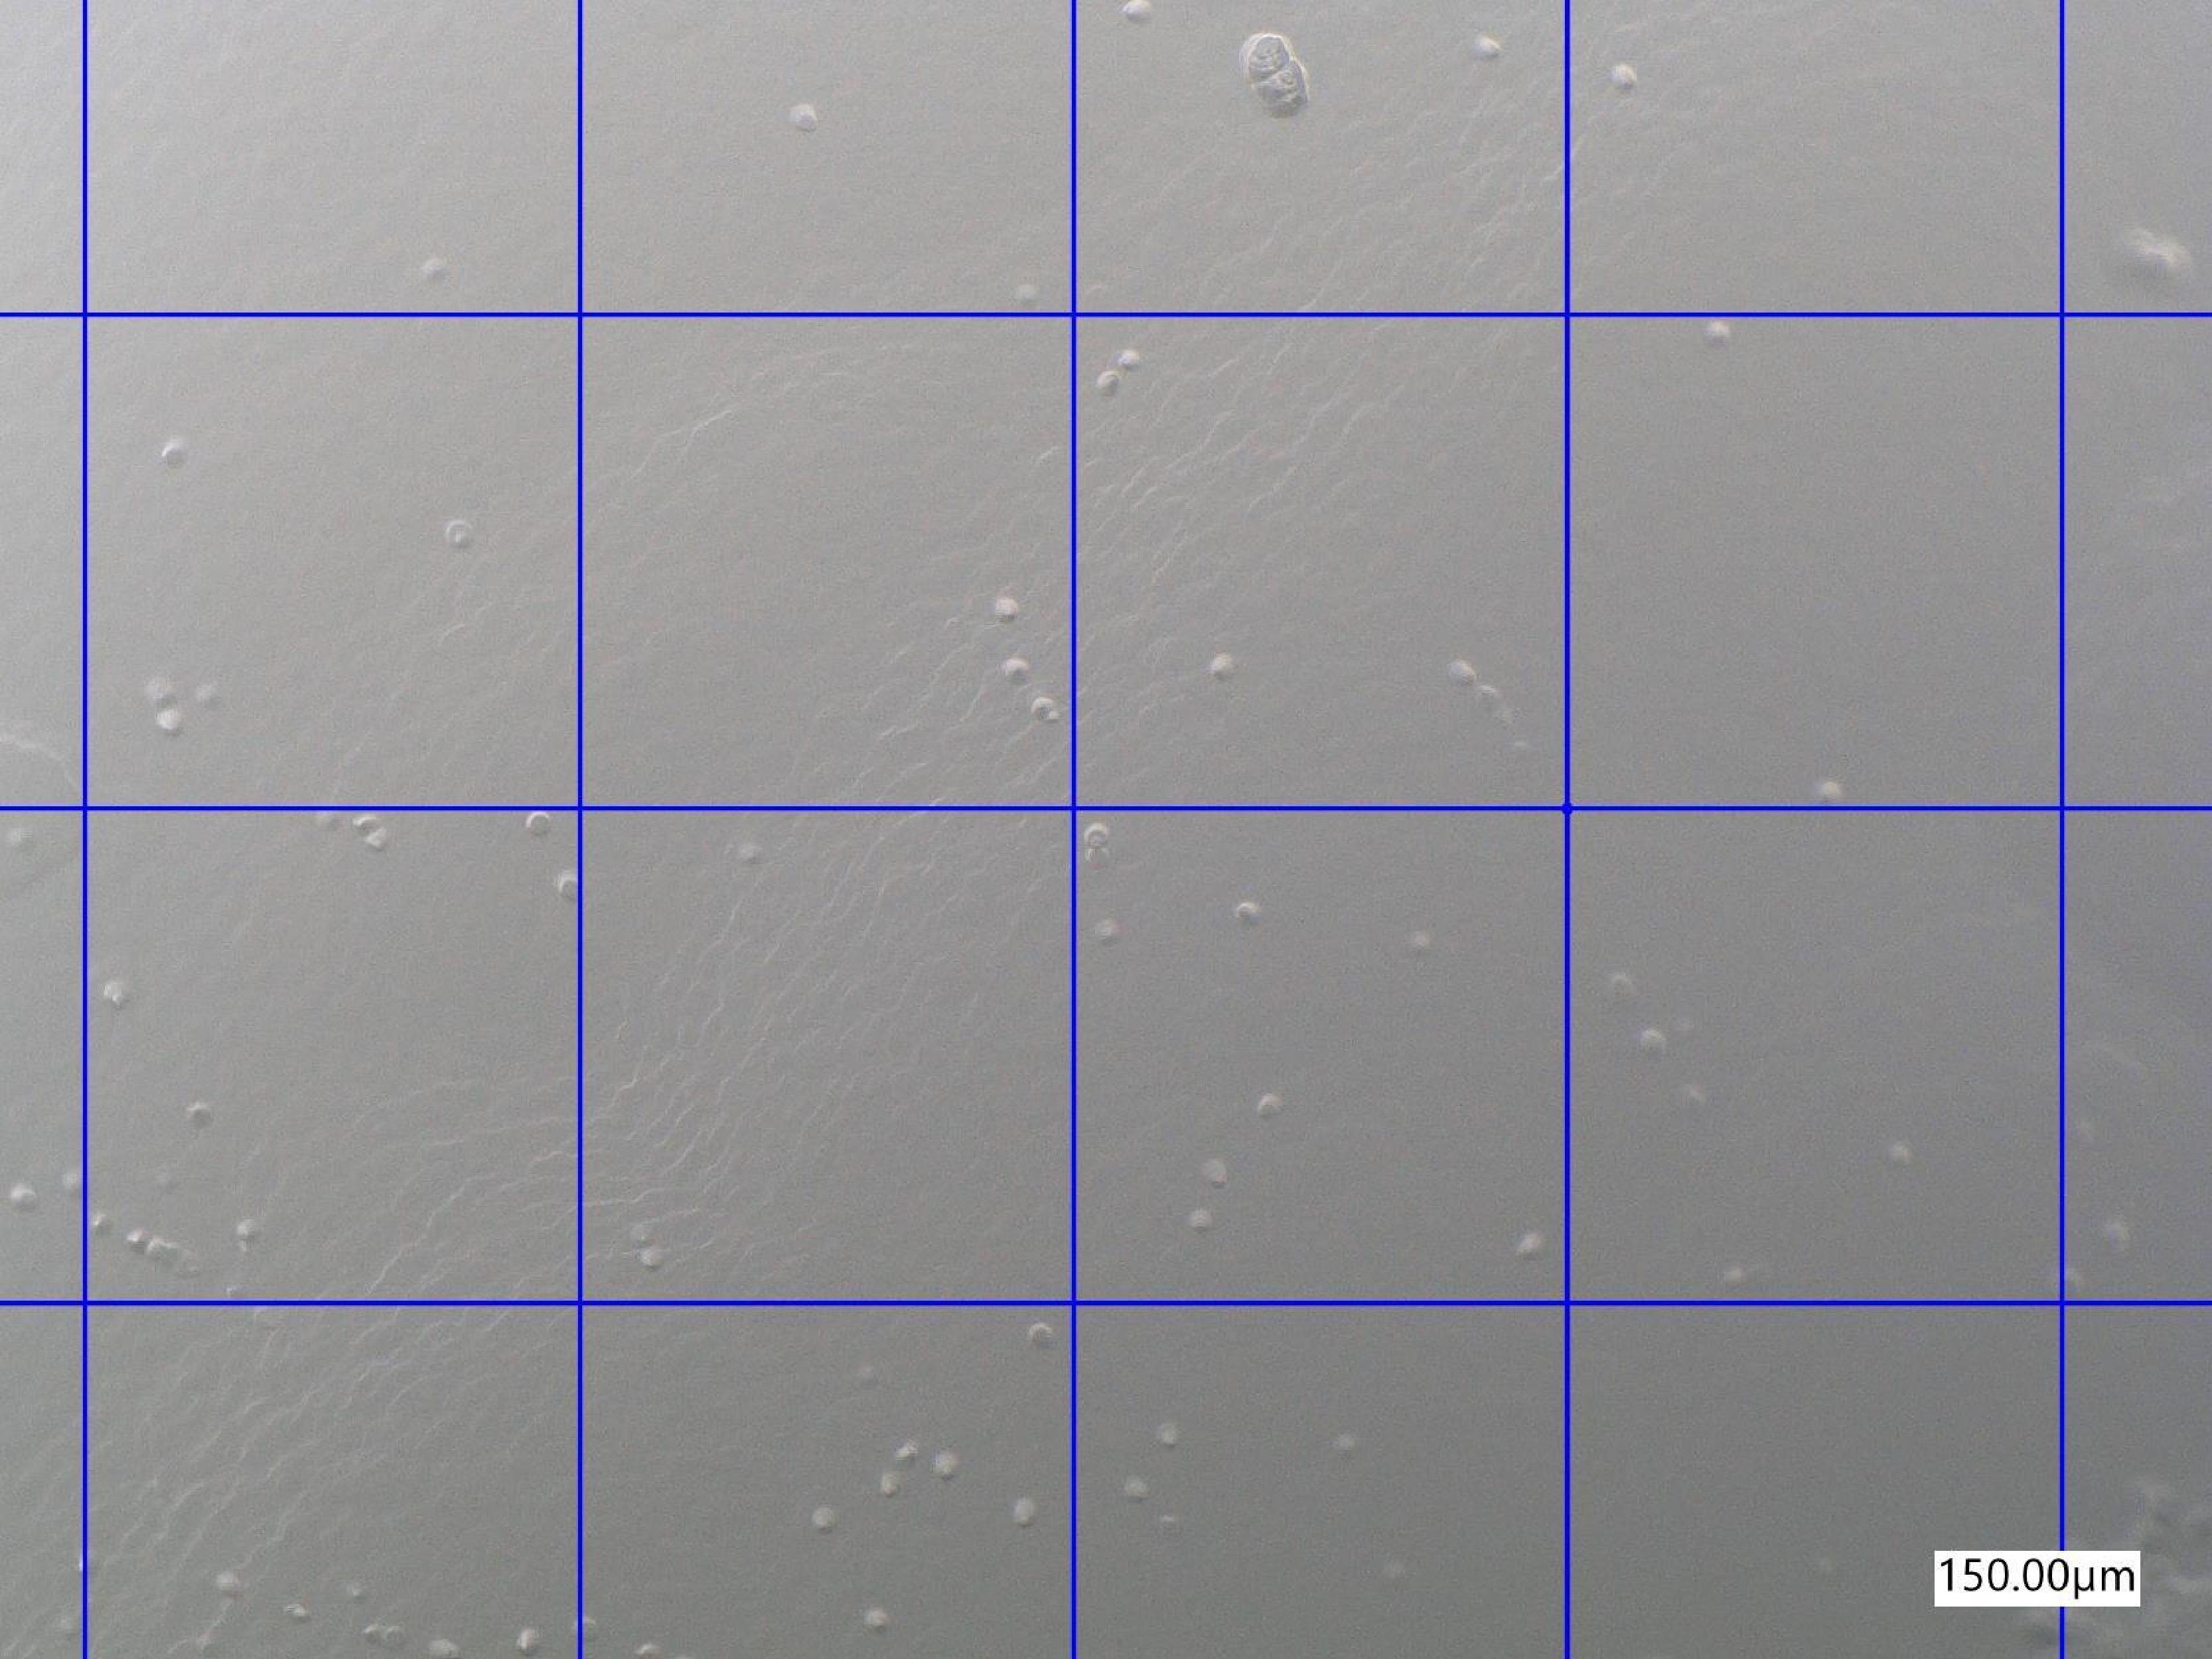
\includegraphics[width=\textwidth]{../media/B2.8/Dichte1_tempered.pdf}
		\caption{Ätzgrübchendichte nicht-getemperte Probe, Aufnahme $1$}
		\label{abb:dichte_t_1}
	\end{minipage}
	\begin{minipage}[t]{.5\linewidth}
		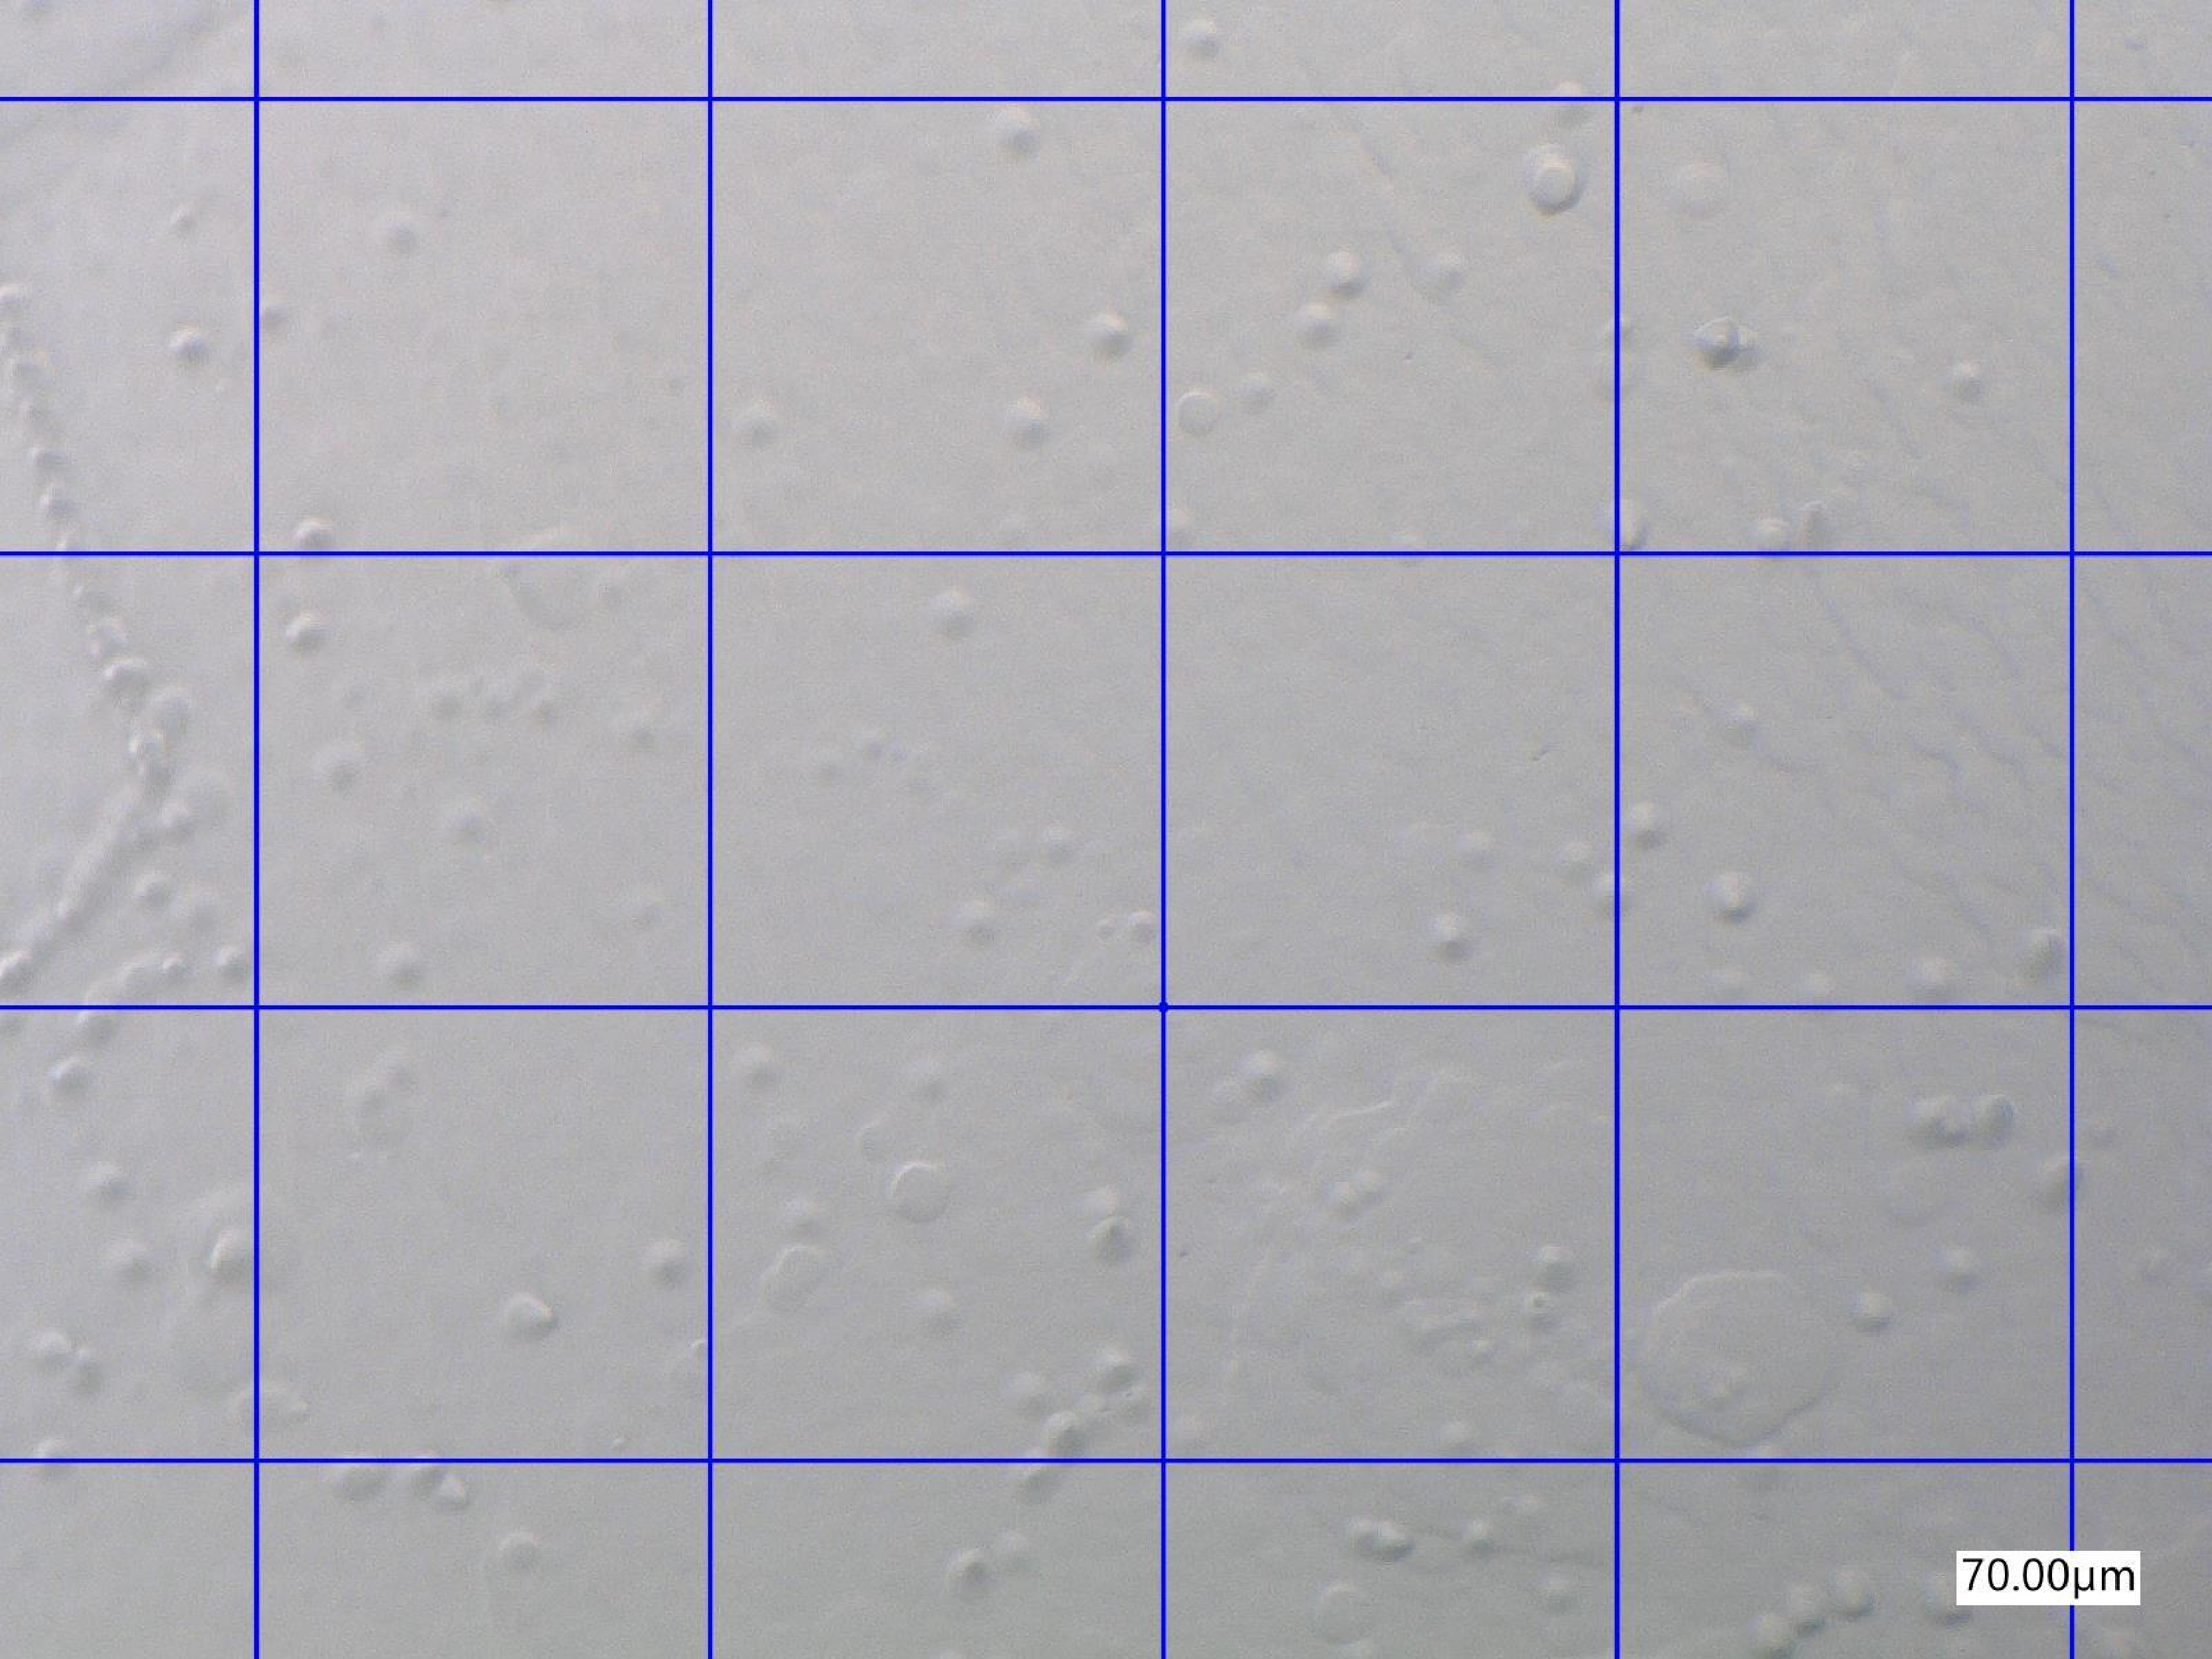
\includegraphics[width=\textwidth]{../media/B2.8/Dichte2_tempered.pdf}
		\caption{Ätzgrübchendichte nicht-getemperte Probe, Aufnahme $2$}
		\label{abb:dichte_t_2}
	\end{minipage}
\end{figure}

Wieder folgt aus den Gleichungen $\eqref{N}$ bis $\eqref{DeltaNbar}$
die mittlere Ätzgrübchendichte $\bar N_\mathrm{t}$ der getemperten
Probe.
\begin{eqnarray}
    N_\mathrm{t,1} &=& (2.8 \pm 0.3) \cdot 10^4 \mathrm{\, cm^{-2}} \\
    N_\mathrm{t,2} &=& (1.4 \pm 0.1) \cdot 10^5 \mathrm{\, cm^{-2}}
    \\
    \bar N_\mathrm{t}
        &=& (8.3 \pm 5.5) \cdot 10^4 \mathrm{\, cm^{-2}}
        \quad(\pm 66.44\,\%)
\end{eqnarray}

\hypertarget{kleinwinkelkorngrenze}{%
\subsection{Kleinwinkelkorngrenze}\label{kleinwinkelkorngrenze}}

Es wurden drei Bilder von Kleinwinkelkorngrenzen aufgenommen. Nun werden die Winkel $\theta$ zwischen den Kristalliten an diesen
Kleinwinkelkorngrenzen bestimmen. Dieser durch Gleichung
\eqref{theta} gegeben, wobei $d$ den Abstand zweier Ätzgrübchen
beschreibt.

Die Ungenauigkeit der Gitterkonstante $\Delta a=1 \cdot 10^{-7} \mathrm{\, \mu m}$ $[5]$ und die des Mikroskops $\Delta d_m = 5 \cdot 10^{-3} \mathrm{\, \mu m}$ ergeben
mittels Gauß'scher Fehlerfortpflanzung die Ungenauigkeit des Winkels
$\Delta \theta$. Wird der Abstand $d_n$ von $n$ Grübchen gemessen,
so sinkt die Ungenauigkeit $\Delta d$ des Abstandes zweier Grübchen.
\begin{eqnarray}
    \Delta d &=& \frac{\Delta d_m}{n} \\
    \Delta \theta &=& \sqrt{
        \left(\frac{\Delta a}{\sqrt{2} \cdot d} \right)^2
            + \left( \frac{a}{\sqrt{2} \cdot d^2} \cdot \Delta d \right)^2 }
            \label{DeltaTheta}
\end{eqnarray}

\begin{figure}[h]
	\begin{minipage}[t]{.31\linewidth}
		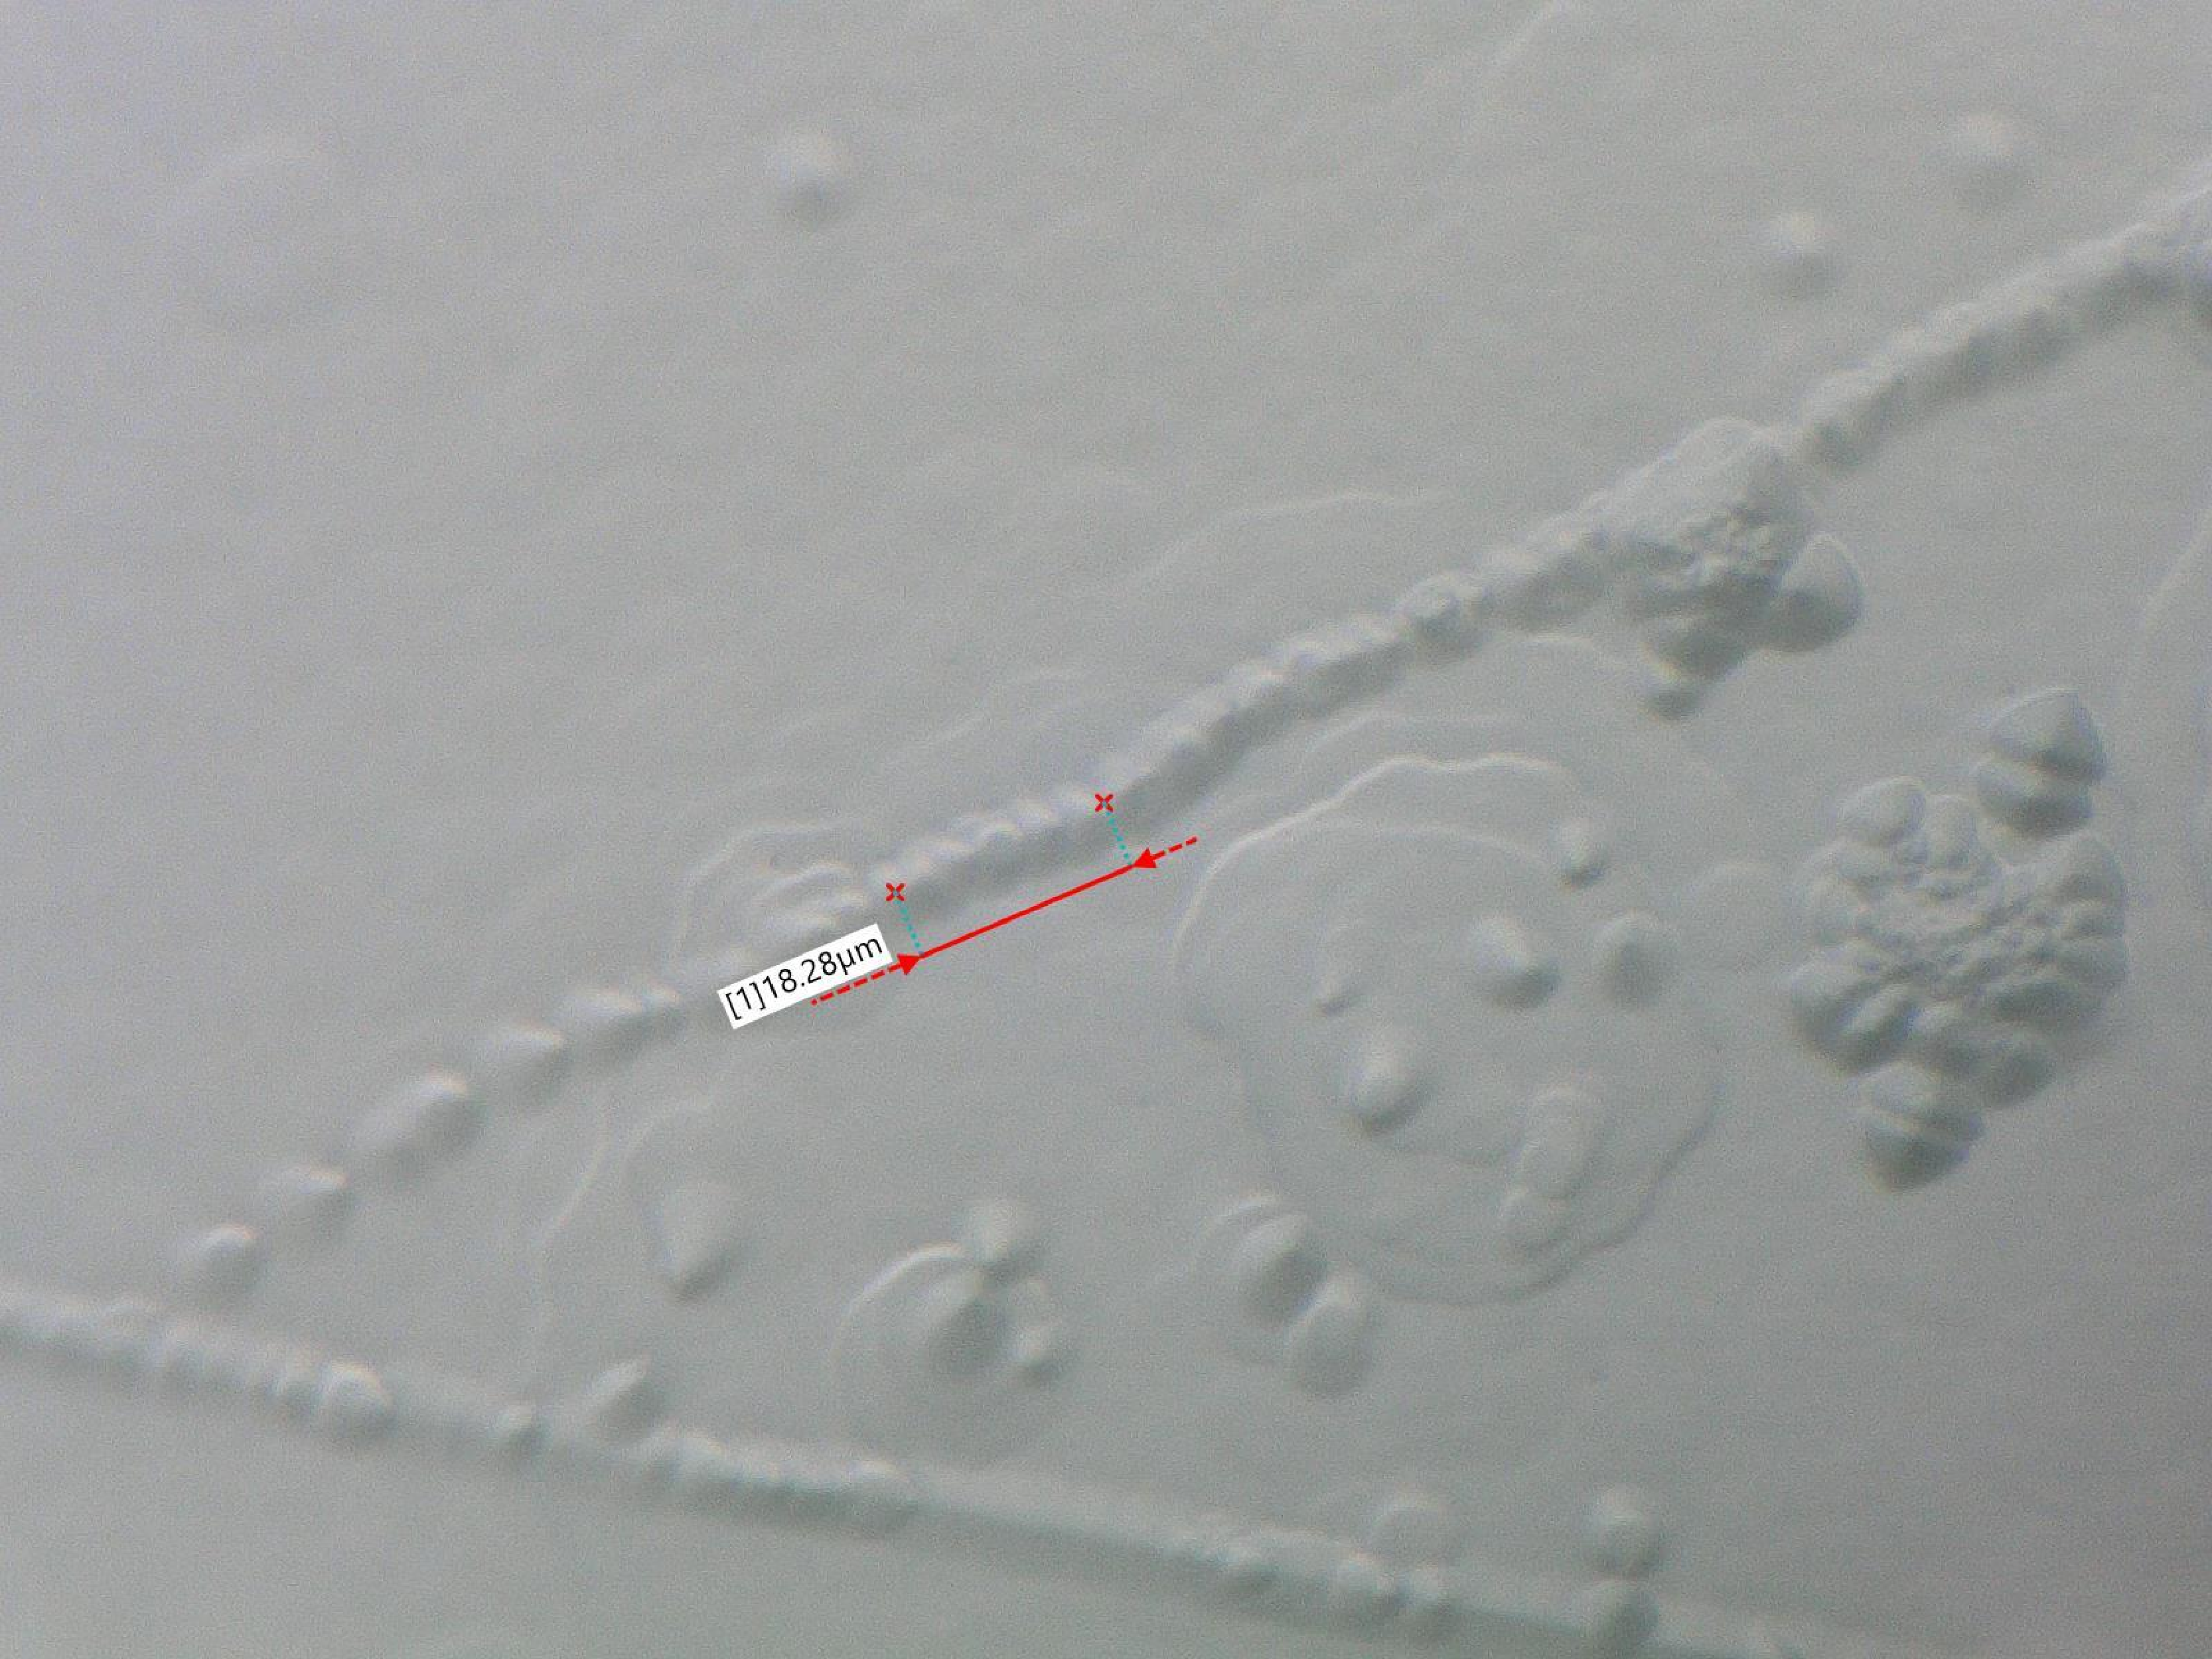
\includegraphics[width=\textwidth]{../media/B2.8/KWK1_tempered.pdf}
		\caption{Messung 1}
		\label{abb:KWK1}
	\end{minipage}
	\begin{minipage}[t]{.31\linewidth}
		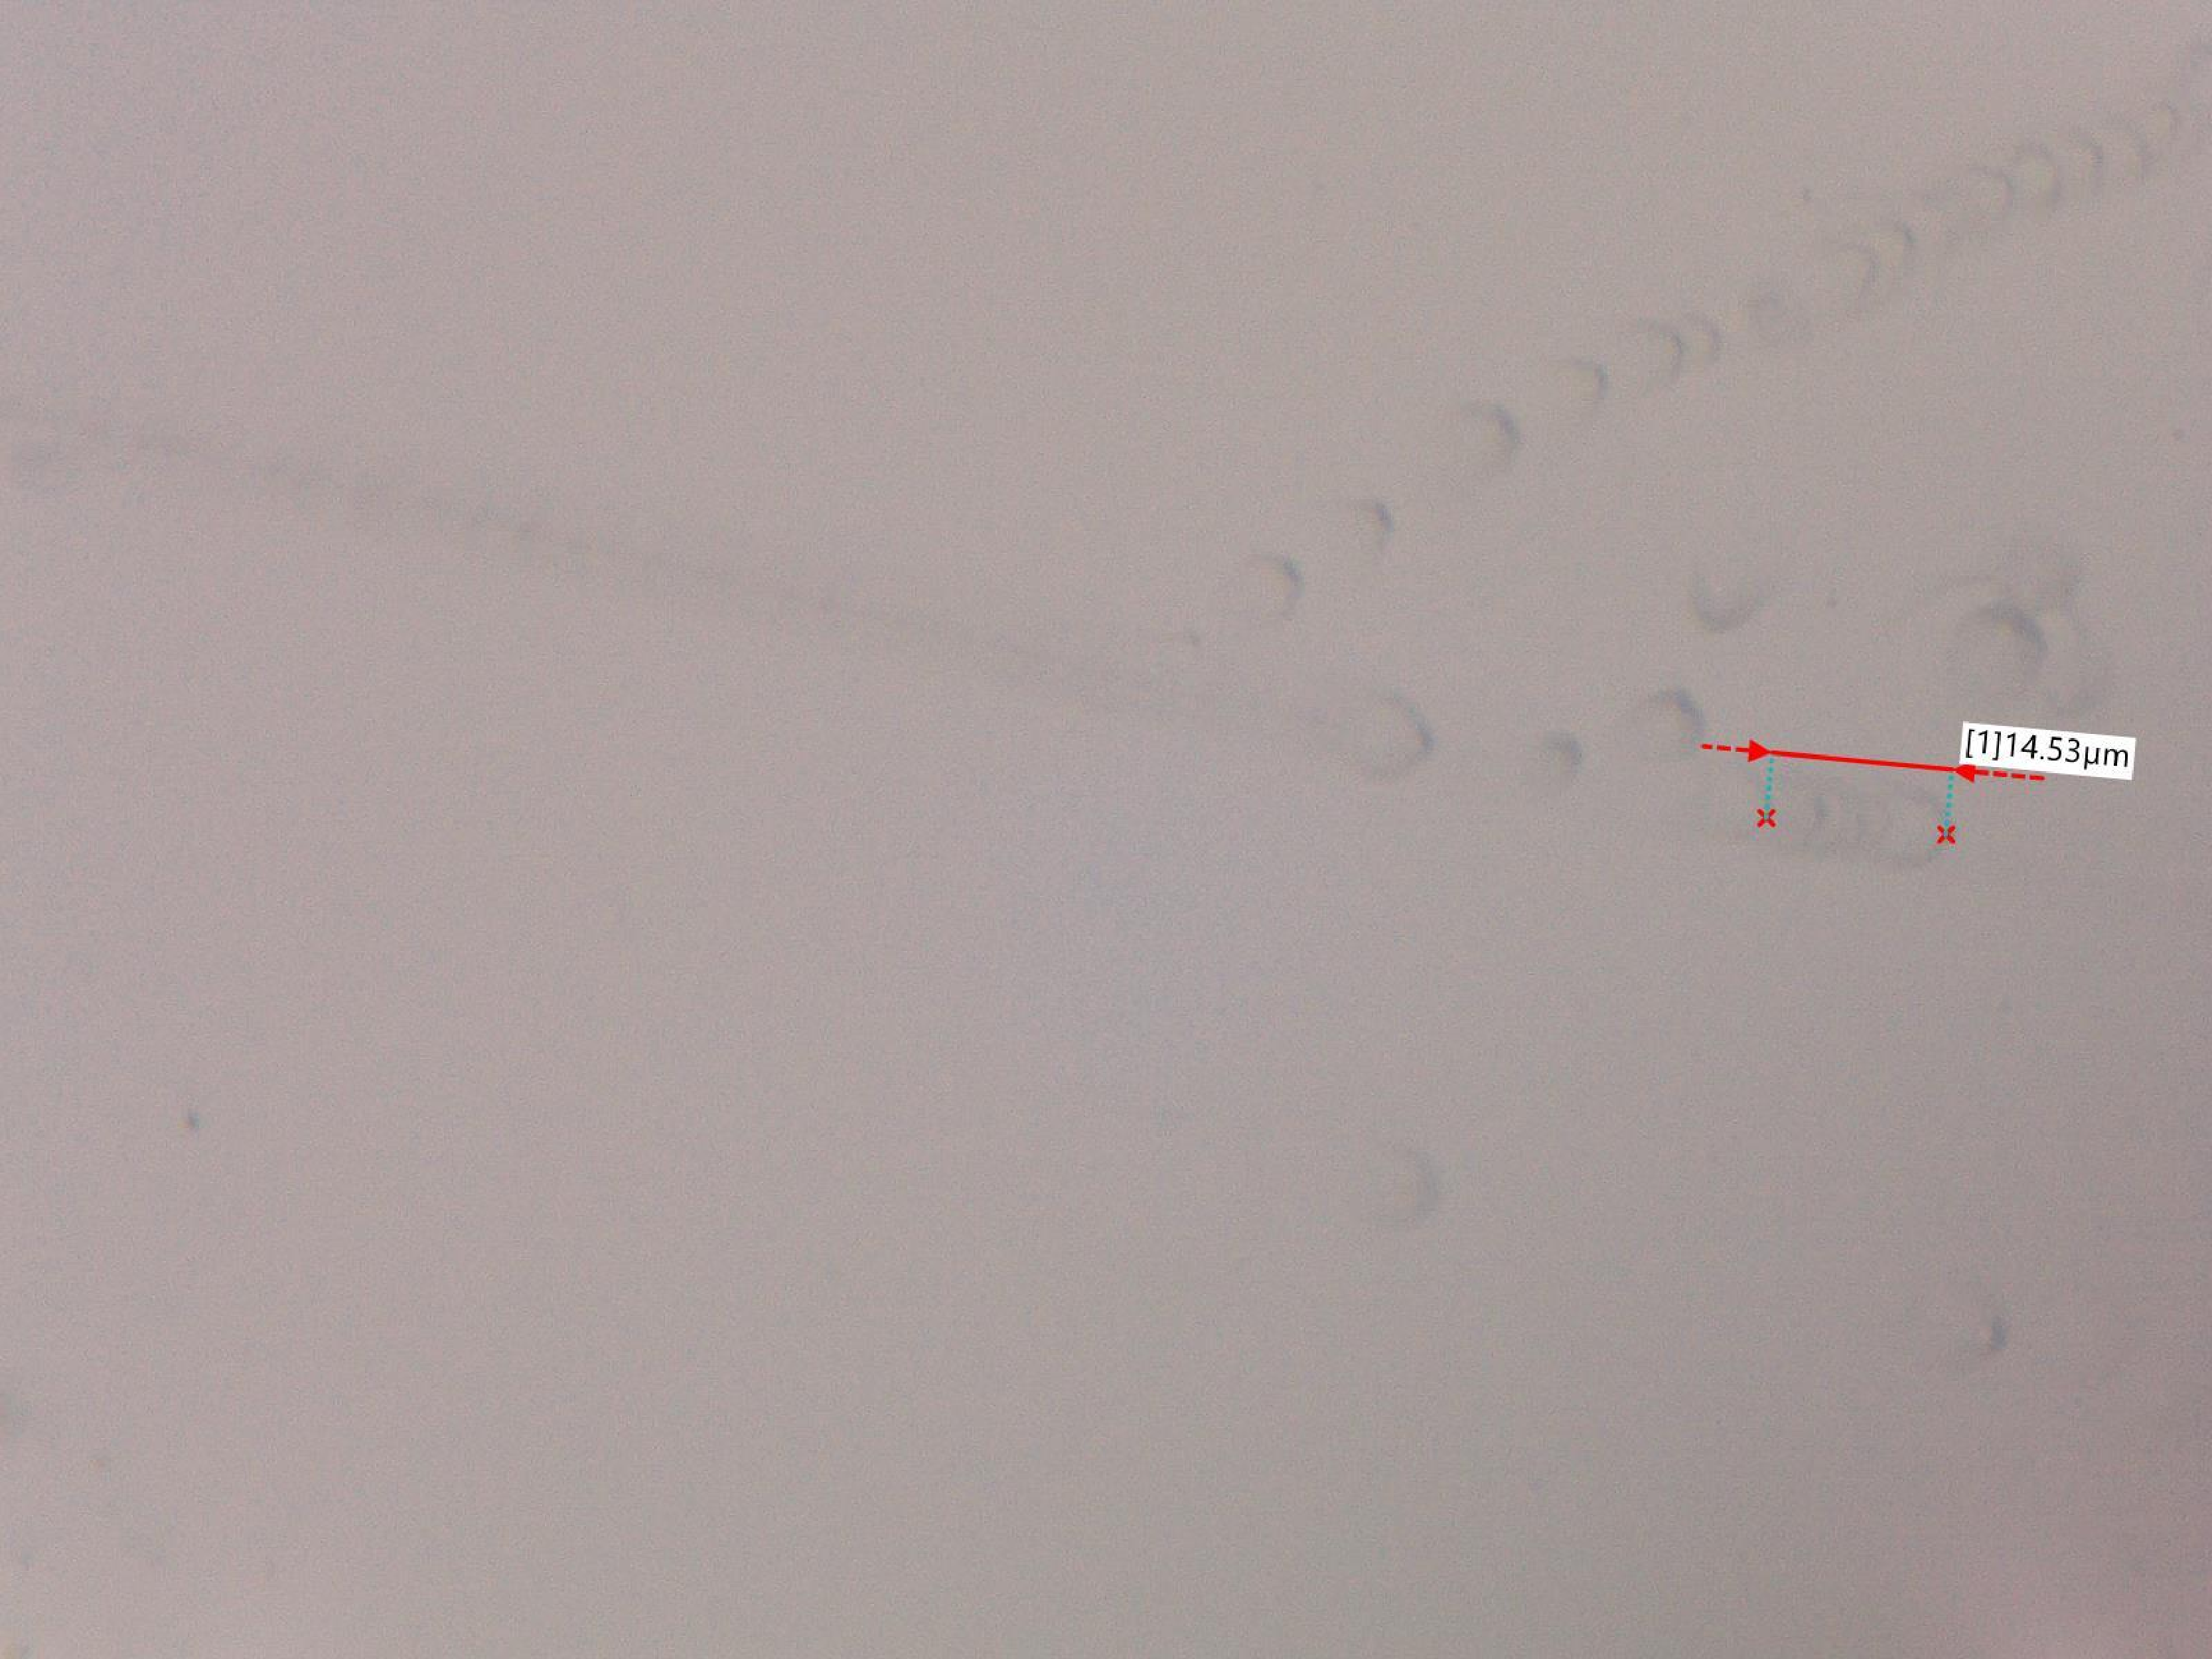
\includegraphics[width=\textwidth]{../media/B2.8/KWK2_tempered.pdf}
		\caption{Messung 2}
		\label{abb:KWK2}
	\end{minipage}
	\begin{minipage}[t]{.31\linewidth}
		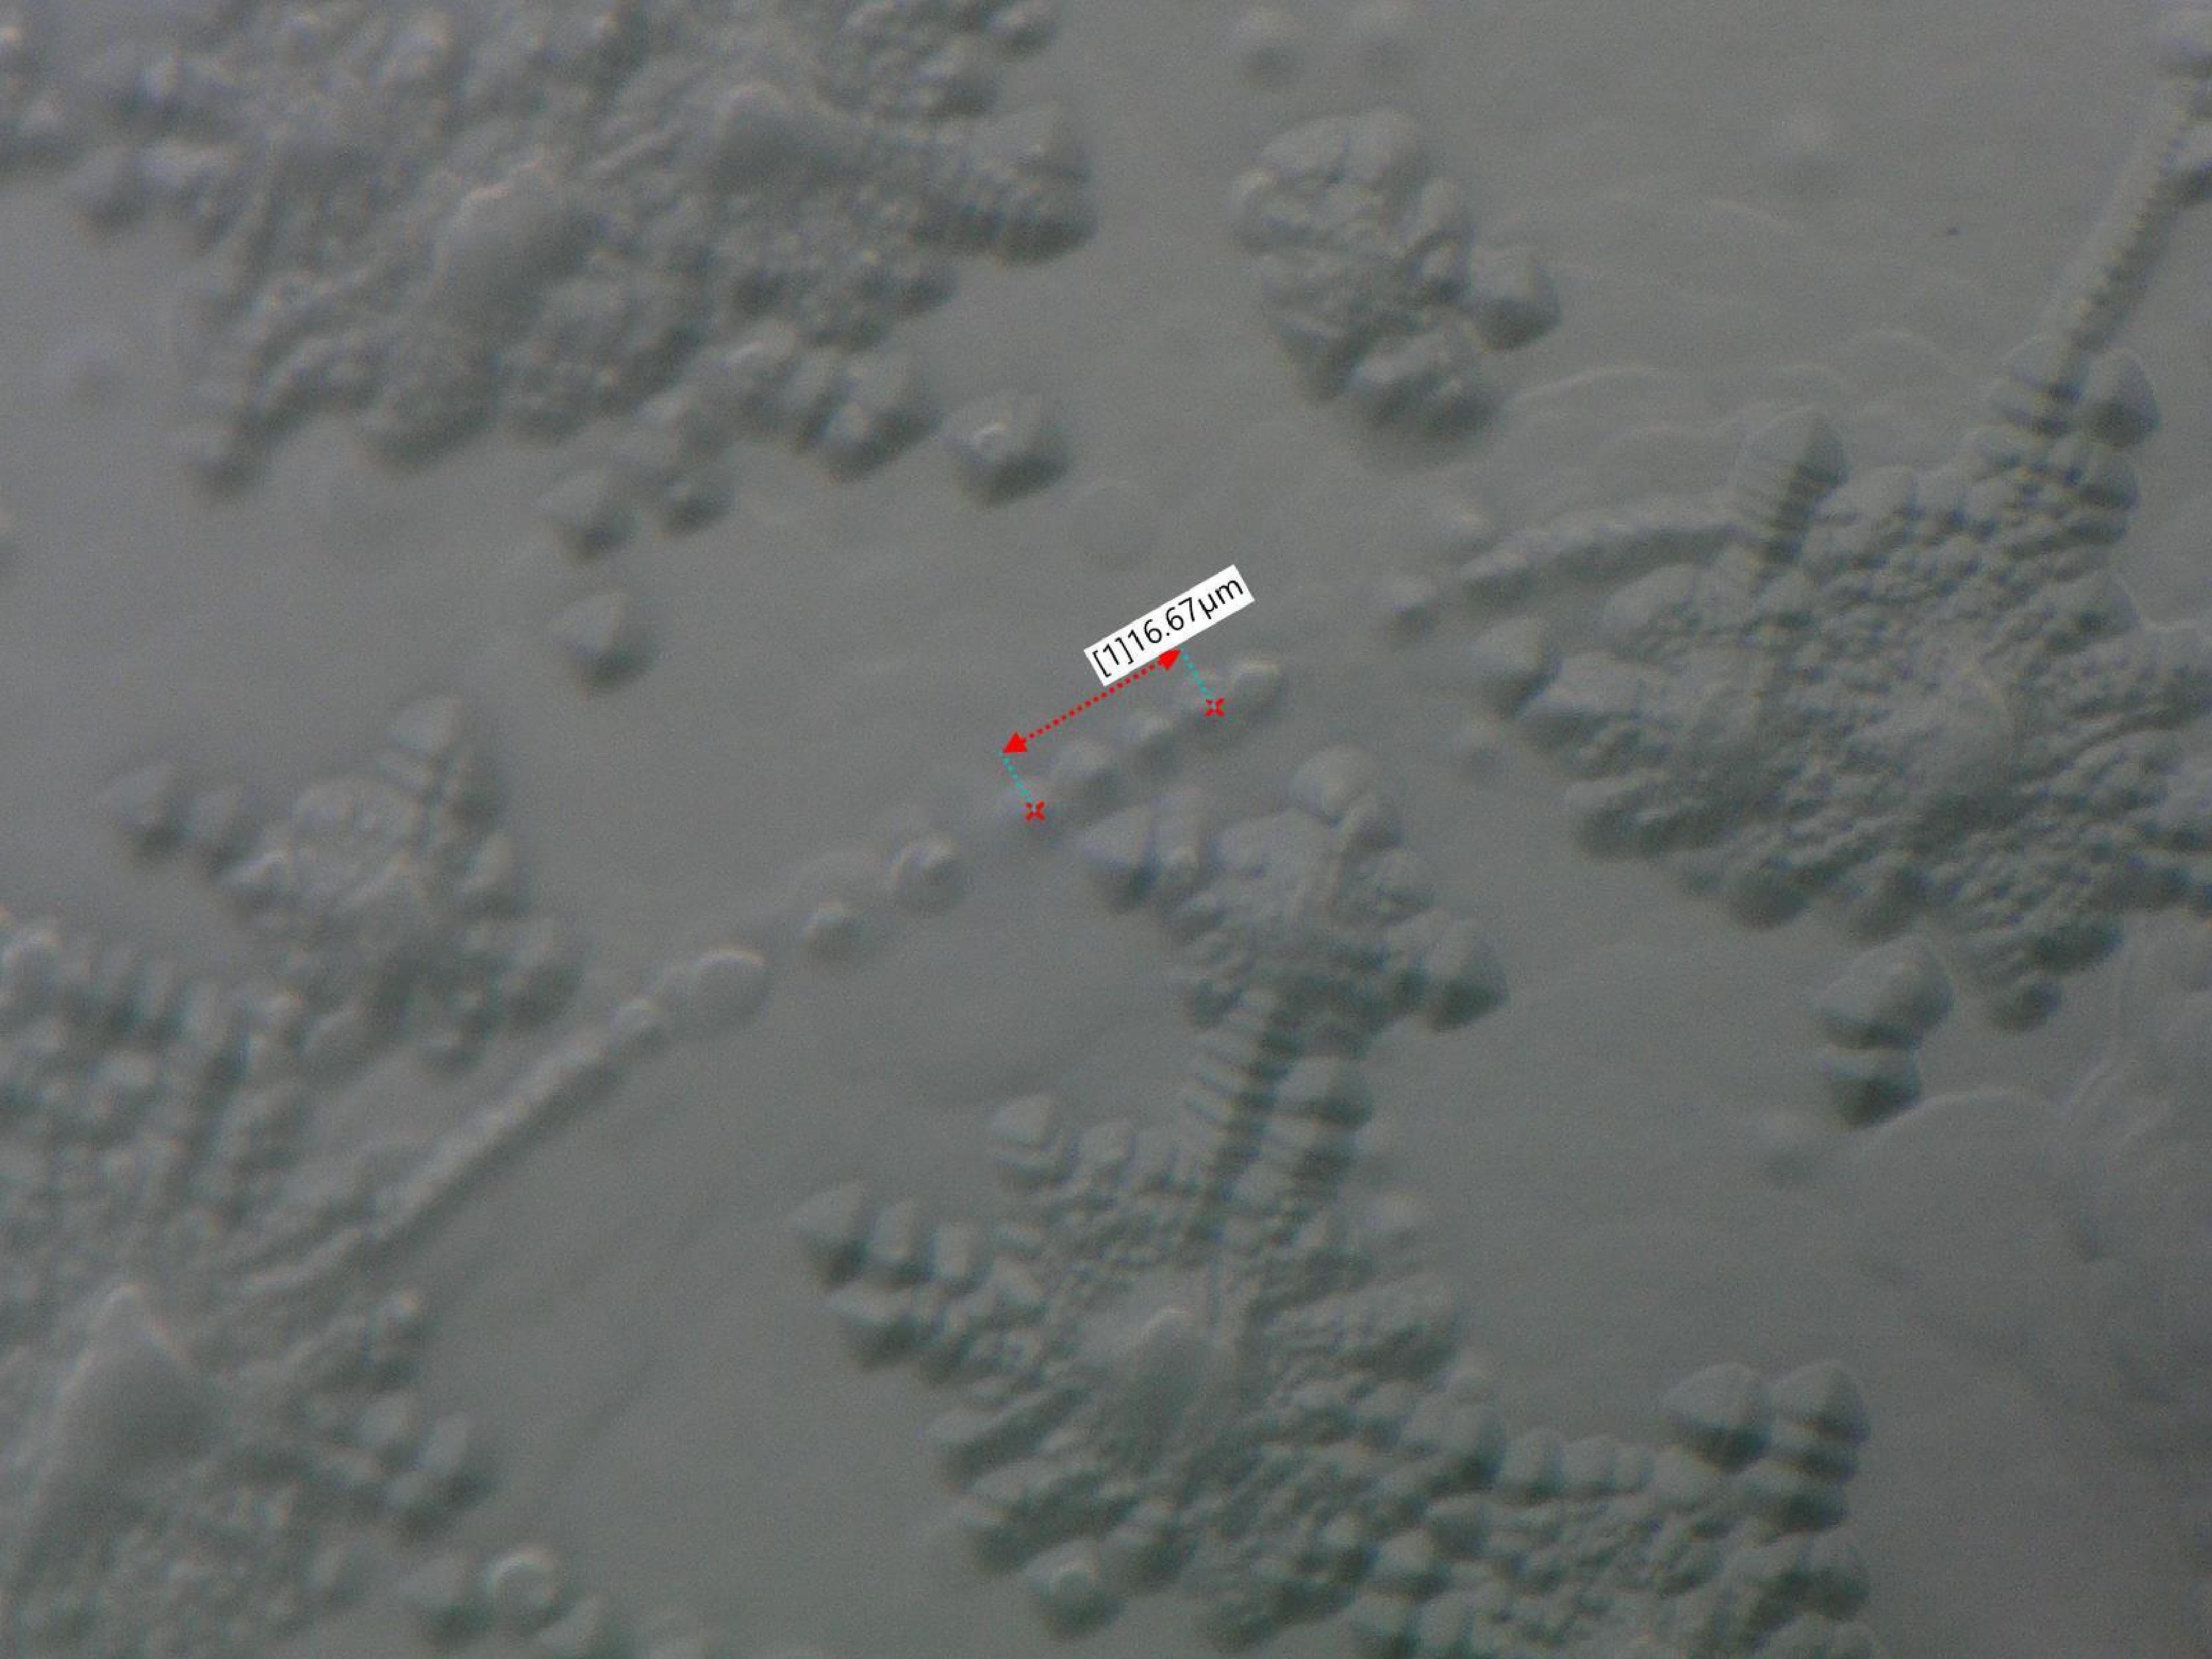
\includegraphics[width=\textwidth]{../media/B2.8/KWK3_tempered.pdf}
		\caption{Messung 3}
		\label{abb:KWK3}
	\end{minipage}
	\caption*{Messungen von Kleinwinkelkorngrenzen}
\end{figure}


\hypertarget{erste-messung}{%
\paragraph*{erste Messung}\label{erste-messung}}

In Abbildung \ref{abb:KWK1} ist die erste Kleinwinkelkorngrenze zu sehen. In
rot ist der Abstand $18.28 \mathrm{\, \mu m}$ für $5$ Ätzgrübchen
eingetragen.

Aus $\eqref{theta}$ und $\eqref{DeltaTheta}$ folgt der erste Abstand
$d_1$, woraus der Winkel $\theta_1$ bestimmt wird.
\begin{eqnarray}
    d_1 &=& (3.656 \pm 0.002) \mathrm{\, \mu m} \\
    \theta_1 &=& (7.775 \pm 0.005) \cdot 10^{-5} \mathrm{\, rad} \\
        &=& (4.455 \pm 0.003) \cdot 10^{-3\ \ \circ}
\end{eqnarray}

\hypertarget{zweite-messung}{%
\paragraph*{zweite Messung}\label{zweite-messung}}

Die zweite von uns aufgenommene Kleinwinkelkorngrenze ist in Abbildung
\ref{abb:KWK2} zu sehen. Hier ist wieder der Abstand von $5$ Ätzgrübchen mit
$14.53 \mathrm{\, \mu m}$ eingetragen.

Der Abstand zweier Ätzgrübchen $d_2$ sowie der Winkel $\theta_2$
werden analog bestimmt.
\begin{eqnarray}
    d_2 & = & (2.096\pm 0.002) \cdot 10^{-3} \mathrm{\, \mu m} \\
    \theta_2 &=& (9.782 \pm 0.008) \cdot 10^{-5} \mathrm{\, rad} \\
        &=& (5.605 \pm 0.005) \cdot 10^{-3\ \circ}
\end{eqnarray}

\hypertarget{dritte-messung}{%
\paragraph*{dritte Messung}\label{dritte-messung}}

An der letzten untersuchten Stelle ist der Abstand für $3$ Ätzgrübchen
von $16.76 \mathrm{\, \mu m}$ zu sehen, siehe Abb. \ref{abb:KWK3}.

Erneut werden der Abstand zweier Ätzgrübchen $d_2$ sowie der Winkel
$\theta_2$ analog bestimmt.
\begin{eqnarray}
    d_3 &=& (5.587 \pm 0.003) \mathrm{\, \mu m} \\
    \theta_3 &=& (5.088 \pm 0.003) \mathrm{\, rad} \\
        &=& (2.915 \pm 0.002) \cdot 10^{-3\ \circ}
\end{eqnarray}

\hypertarget{nadeldruckrosetten-1}{%
\subsection{Nadeldruckrosetten}\label{nadeldruckrosetten-1}}

Die Mikroskopbilder von allen drei Rosetten sind zusammen und einzeln in
den Abbildungen \ref{abb:Rosetten all} -- \ref{abb:Rosetten 3} zu sehen.

\begin{figure}[ht]
	\begin{minipage}[t]{.5\linewidth}
		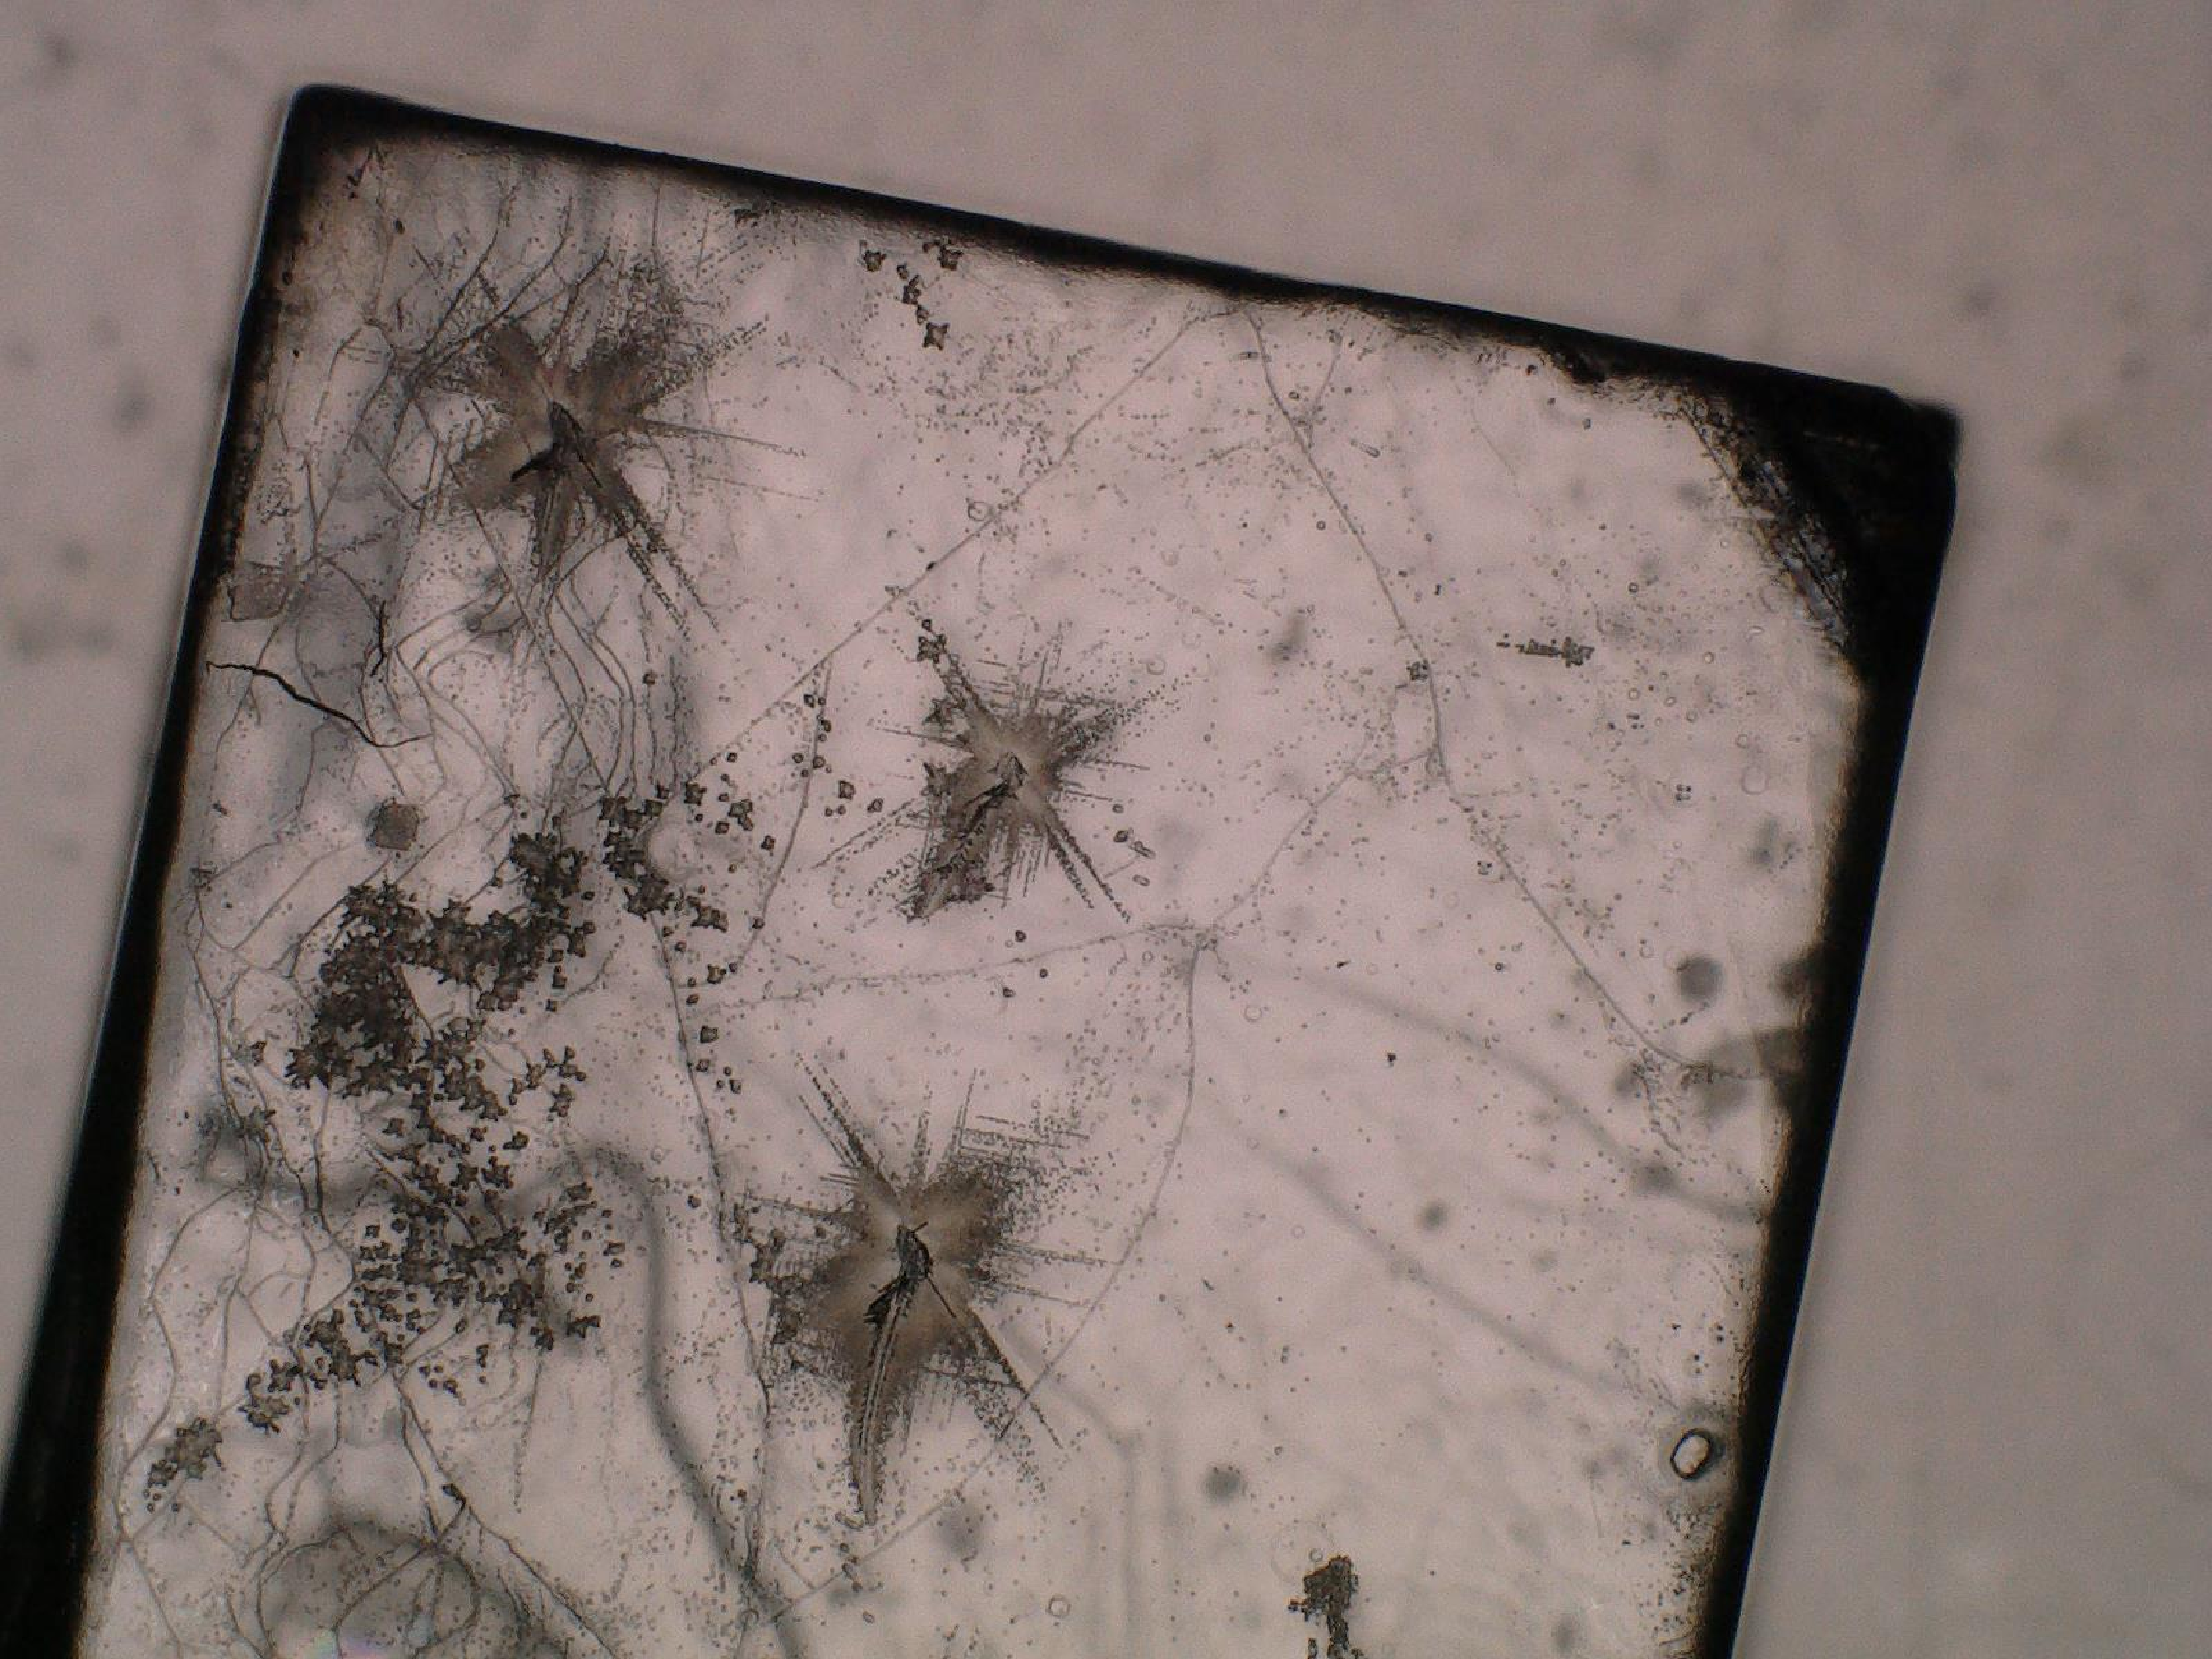
\includegraphics[width=\textwidth]{../media/B2.8/Rosetten_uebersicht.pdf}
		\caption{Nadeldruckrosetten}
		\label{abb:Rosetten all}
	\end{minipage}
	\begin{minipage}[t]{.5\linewidth}
		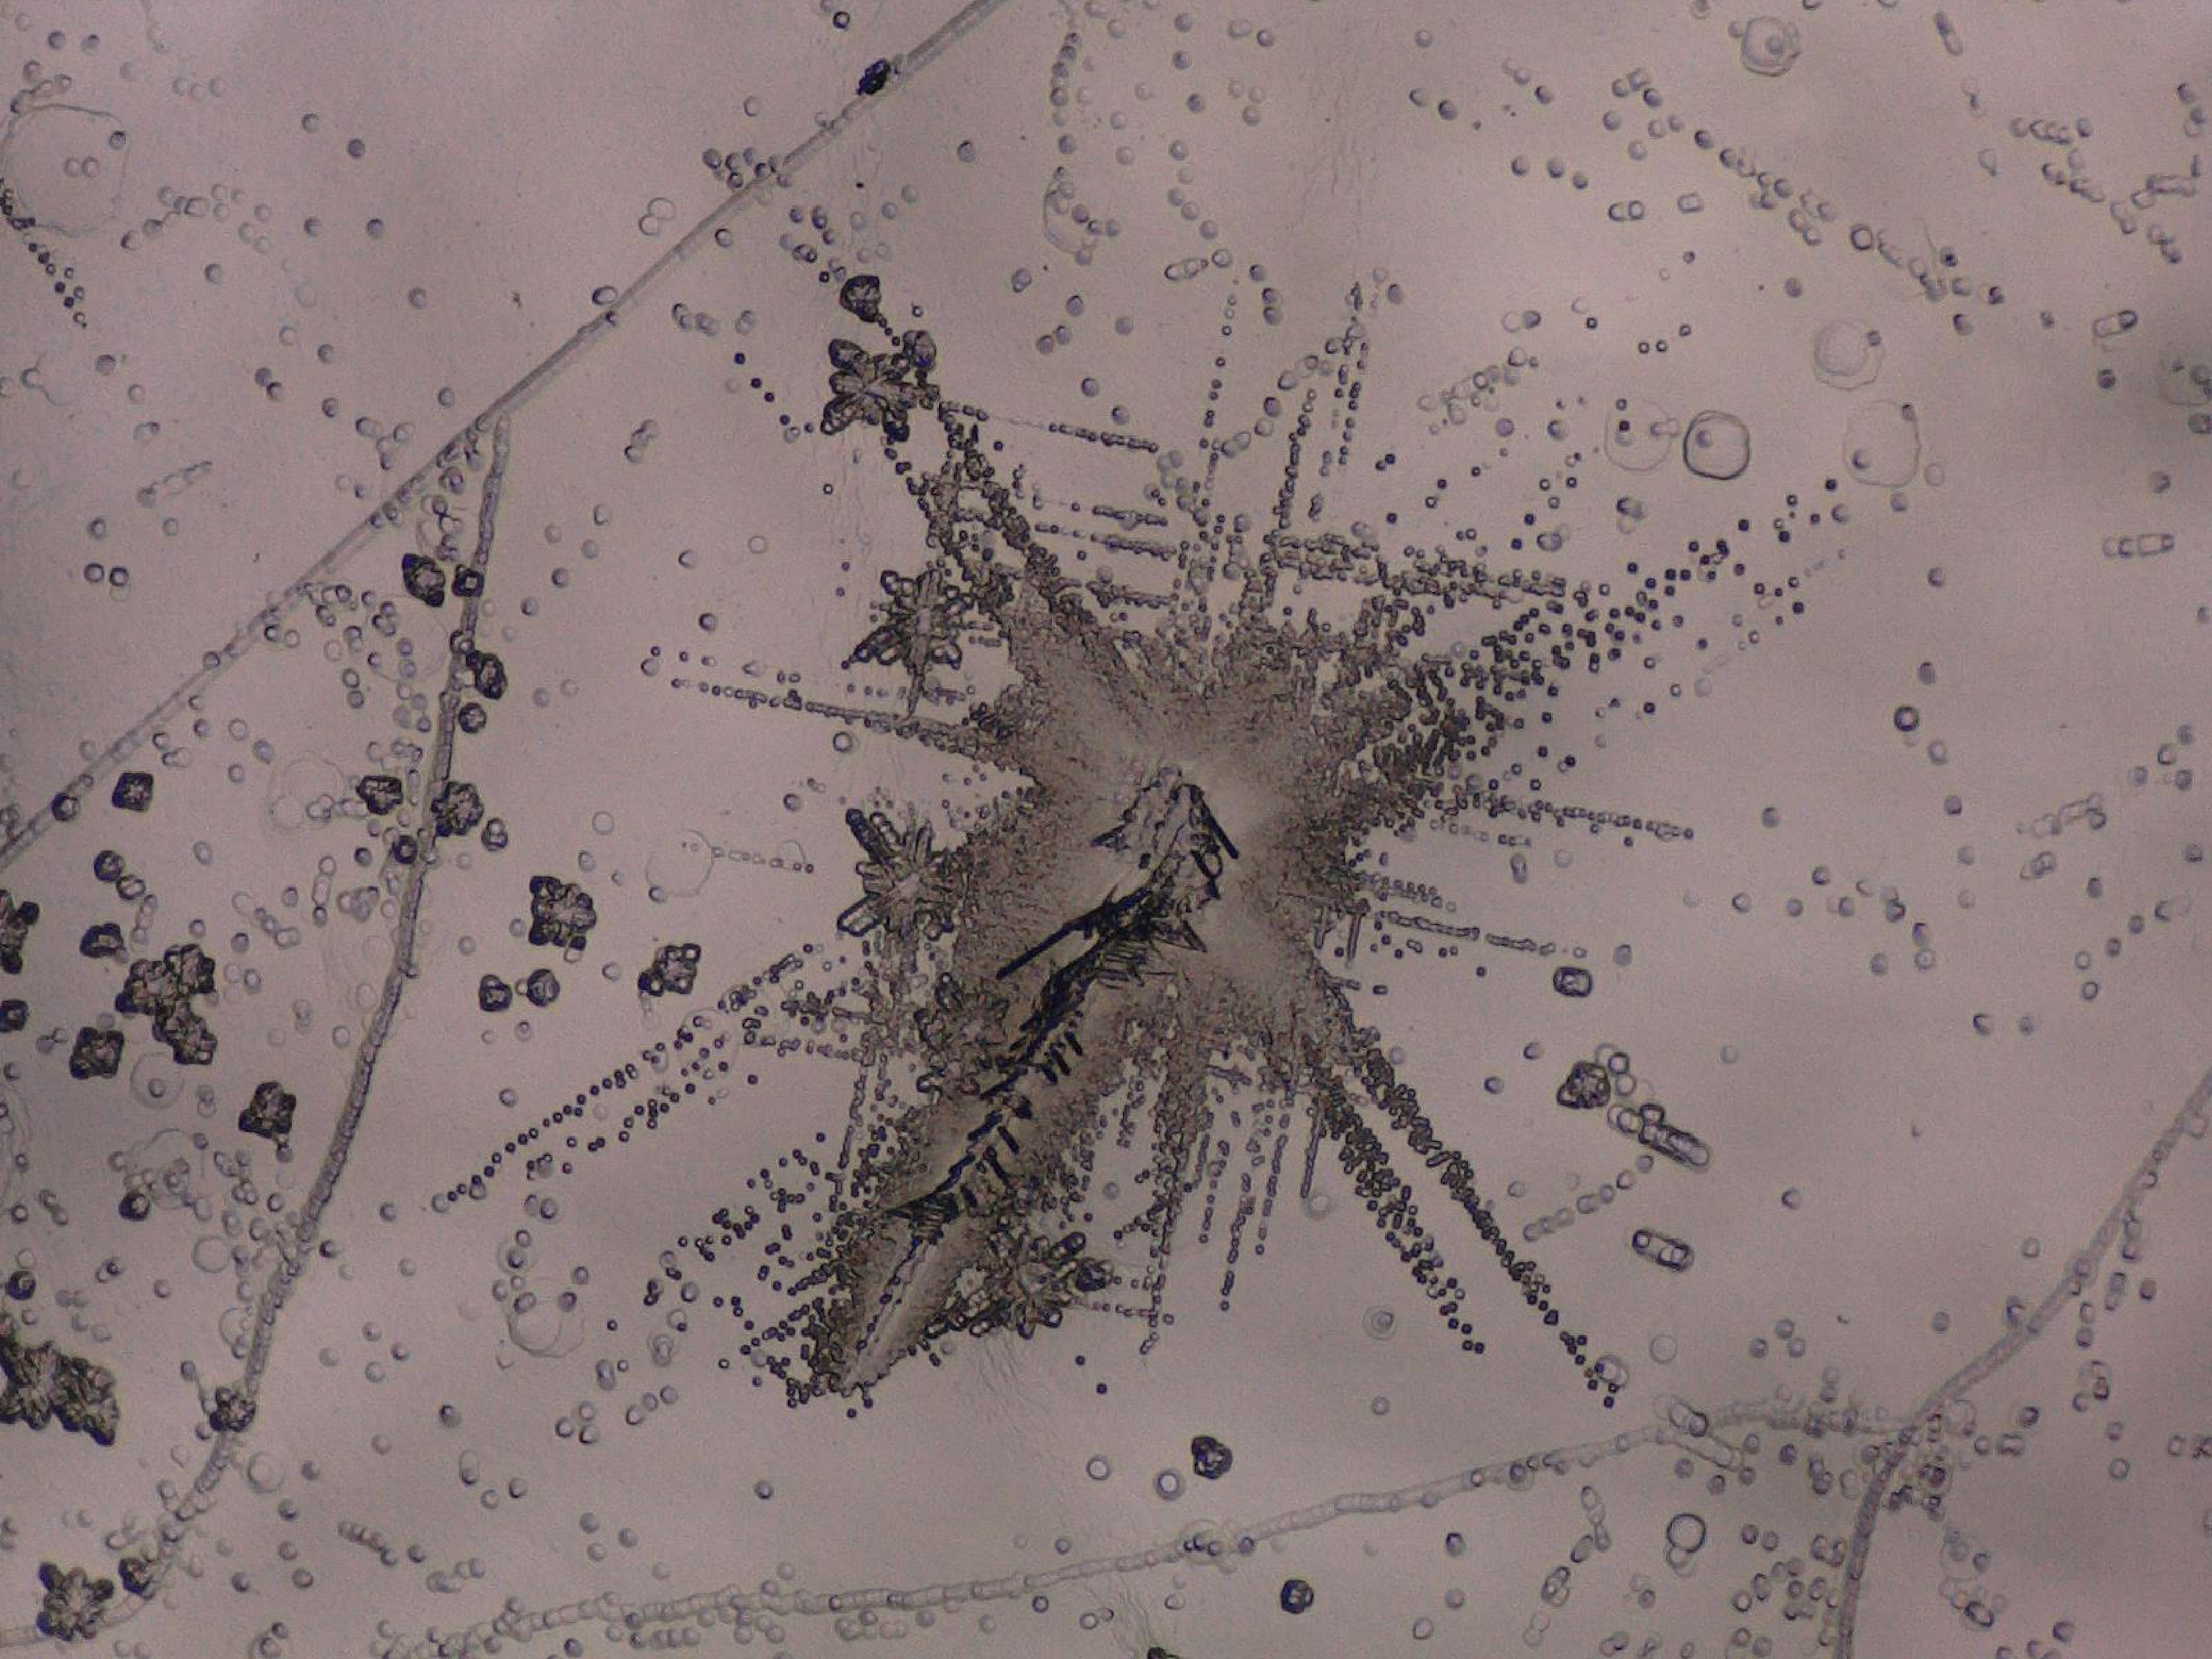
\includegraphics[width=\textwidth]{../media/B2.8/Rosetten_1.pdf}
		\caption{Rosette $1$: obere Mitte }
		\label{abb:Rosetten 1}
	\end{minipage}
	
	\vspace{8pt}
	\begin{minipage}[t]{.5\linewidth}
		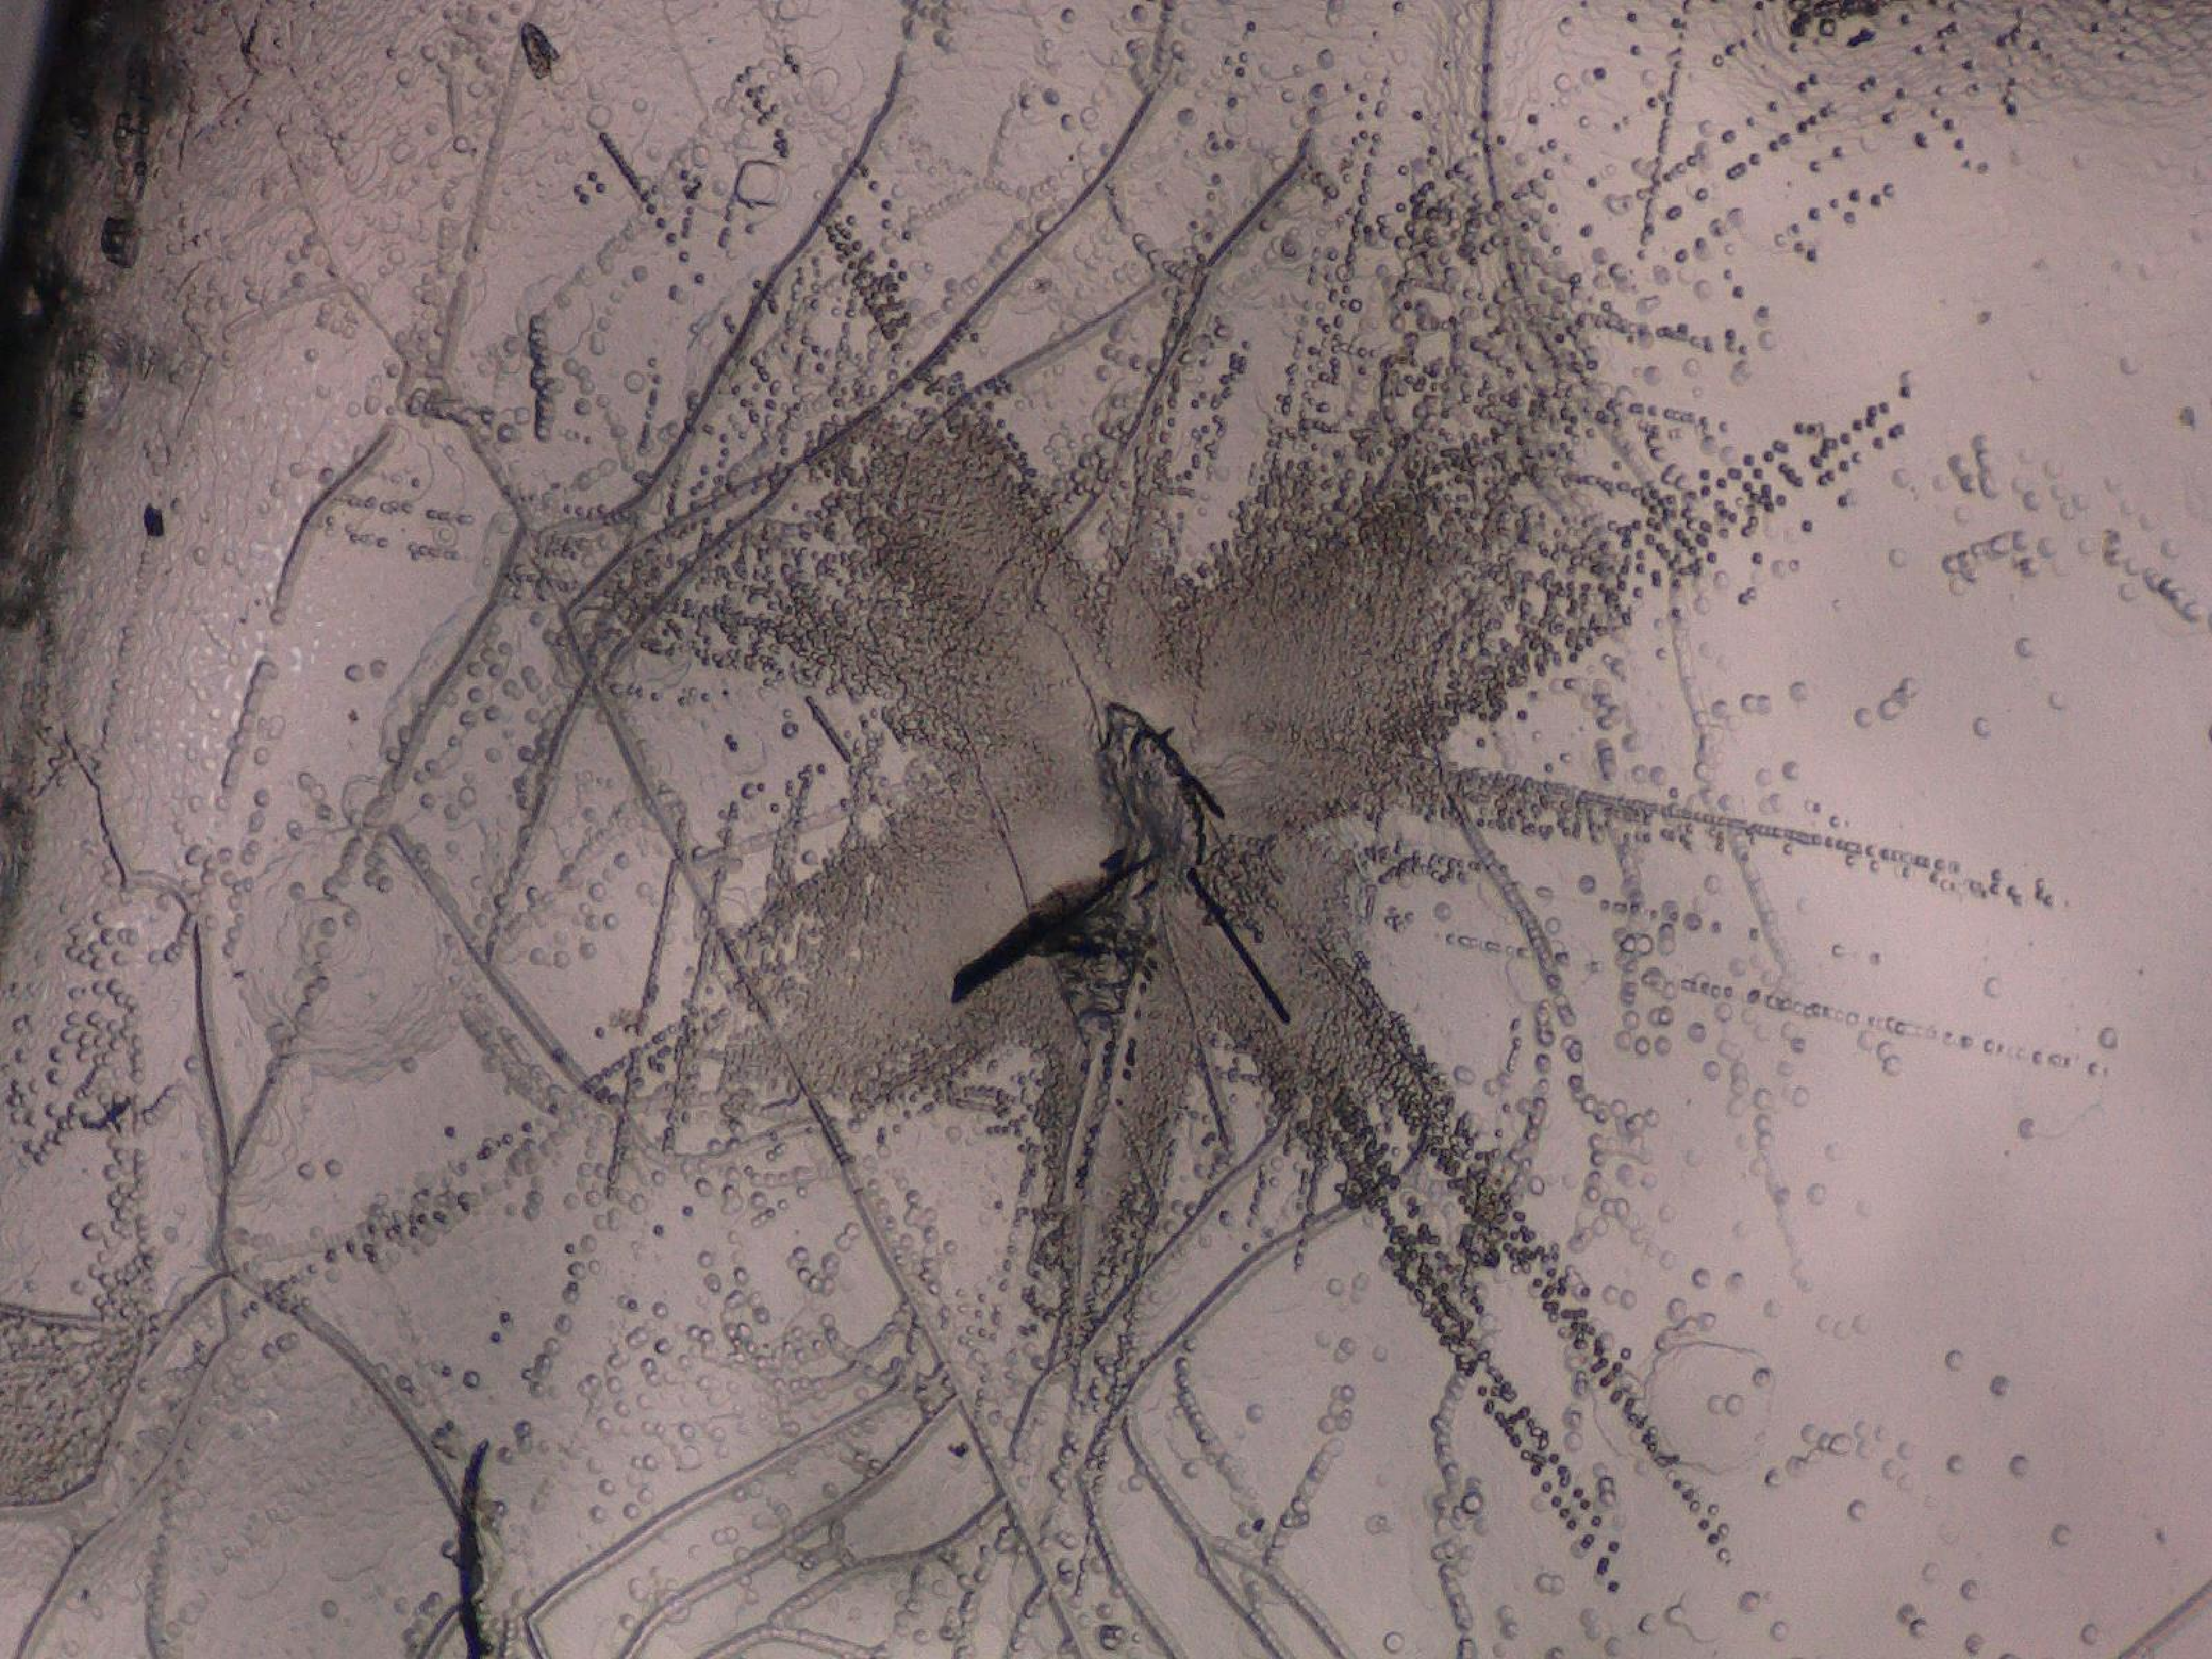
\includegraphics[width=\textwidth]{../media/B2.8/Rosetten_2.pdf}
		\caption{Rosette $2$: Ecke}
		\label{abb:Rosetten 2}
	\end{minipage}
	\begin{minipage}[t]{.5\linewidth}
	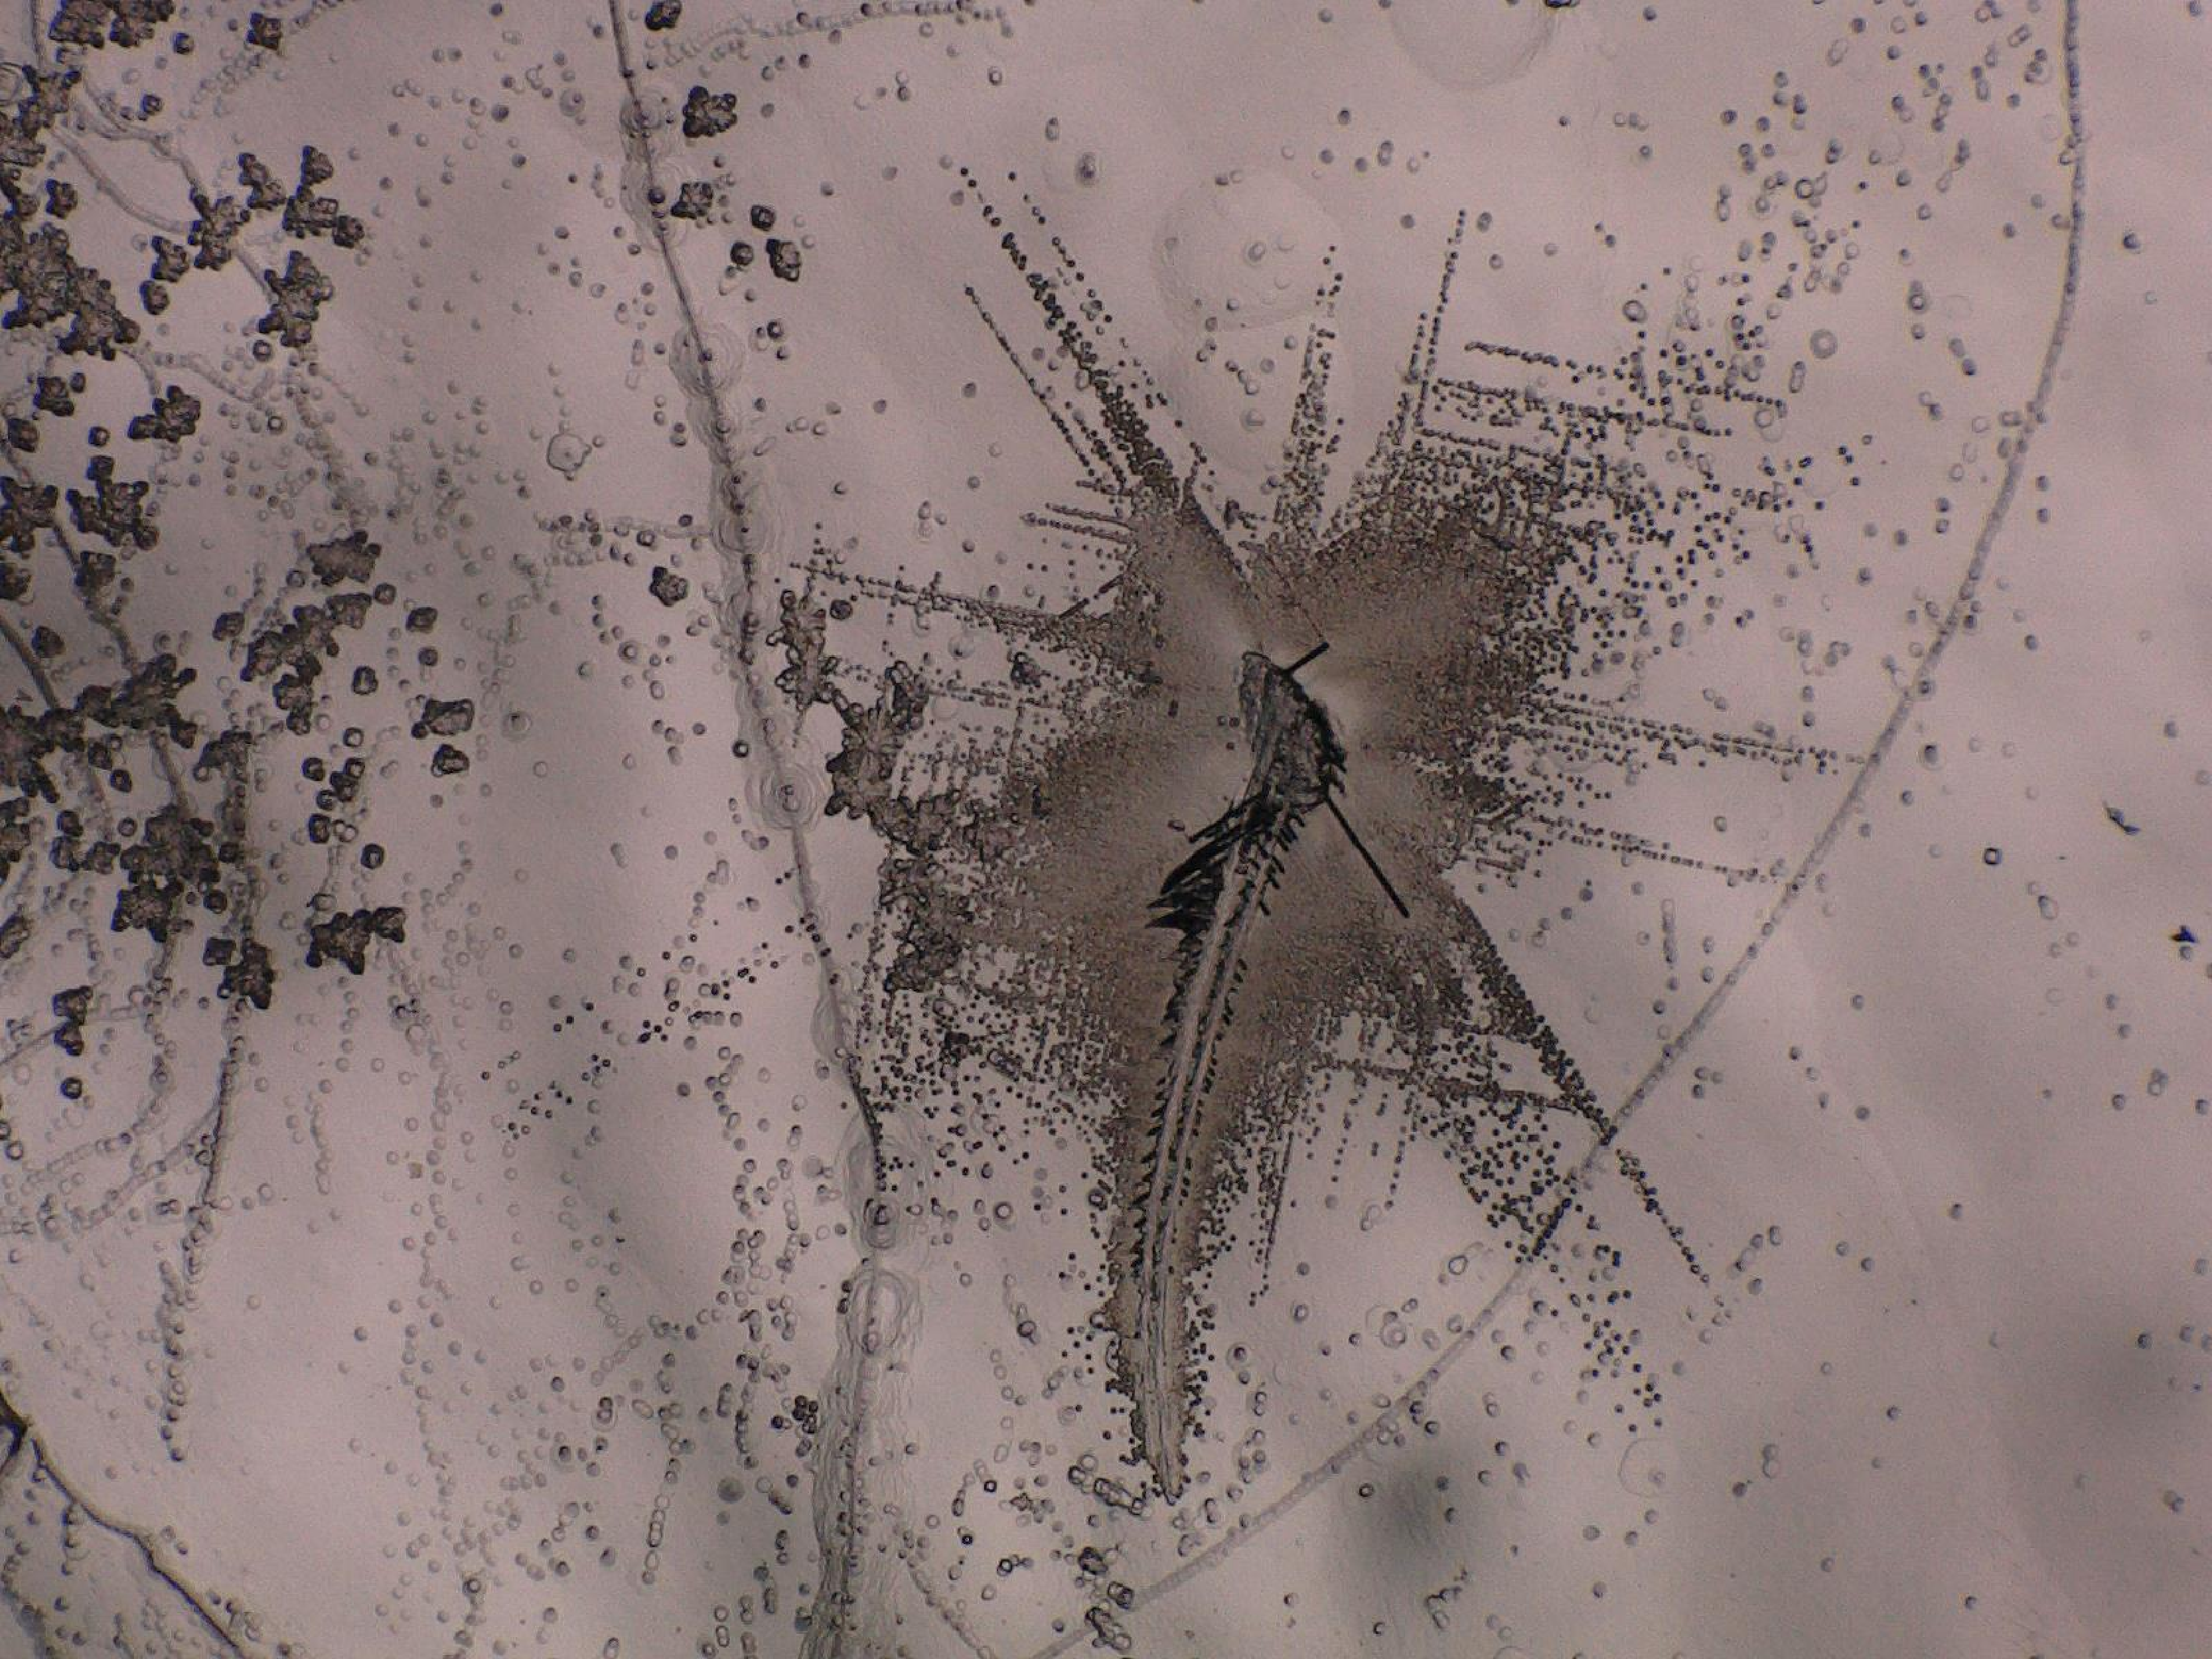
\includegraphics[width=\textwidth]{../media/B2.8/Rosetten_3.pdf}
	\caption{Rosette $3$: Zentrum}
	\label{abb:Rosetten 3}
\end{minipage}
\end{figure}

Entsprechend der Theorie kann man erkennen, dass die Ätzgrübchen entlang bestimmten Richtungen verlaufen. Zudem sieht man in Abbildung \ref{abb:Rosetten 3}, dass die Nadel an der dritten Stelle im Zentrum abgerutscht ist.

\hypertarget{versetzungswanderung}{%
\subsection{Versetzungswanderung}\label{versetzungswanderung}}

Nachdem die Probe für zwei Minuten in der Presse stand, werden die
$\lbrace1\,1\,0\rbrace$-Ebenen als Gleitebenen aktiviert und man
erkennt die Versetzungslinien in verschiedene Richtungen in Abbildung \ref{abb:Druck all}.

Allerdings verlaufen auch einige dieser Versetzungslinien parallel zu
unseren Versetzungsarmen der Rosetten und man kann nicht eindeutig
darüber aussagen, ob die Ätzgrüchen nun zu Versetzungslinien oder zu
Versetzungsarmen gehören. Vergleicht man die Bilder von vorher und
nachher kann man dennoch sagen, dass die Versetzung bei einigen Armen
weiter gewandert ist. Beispielsweise ist der untere Arm der oberen
Diagonalen und der obere Arm der unteren Diagonalen gewandert.

Die Arme in $\expval{1\,1\,0}$-Richtungen sind mehr gewachsen als die
in $\expval{1\,0\,0}$-Richtungen, was man deutlich in den Abbildungen
sieht, dies lässt sich auch mit dem Burgersvektor vereinbaren.

Die Arme zeigen jeweils zur Mitte hin und von der Mitte weg, denn sonst
würden sie sich gegenseitig auslöschen und der Kristall würde sich nicht
verkürzen. Nur in den Bereichen, wo die Versetzung wandert, existieren
eingeschobene Halbebenen, die das Wandern ermöglichen.

Nach der Theorie müssten die Arme aber andersherum wachsen,\footnote{vergleiche Abschnitt \ref{gleitsysteme-bei-mechanischer-belastung}: \nameref{gleitsysteme-bei-mechanischer-belastung}} also wie in
der Abbildung \ref{abb:Rosette}. Es ist jedoch schwierig die, Grübchen richtig
zuzuordnen, und möglicherweise müsste man die Probe länger in der Presse
lassen, um die Effekte deutlicher sehen zu können.

\begin{figure}[ht]
	\begin{minipage}[t]{\linewidth}
		\centering
		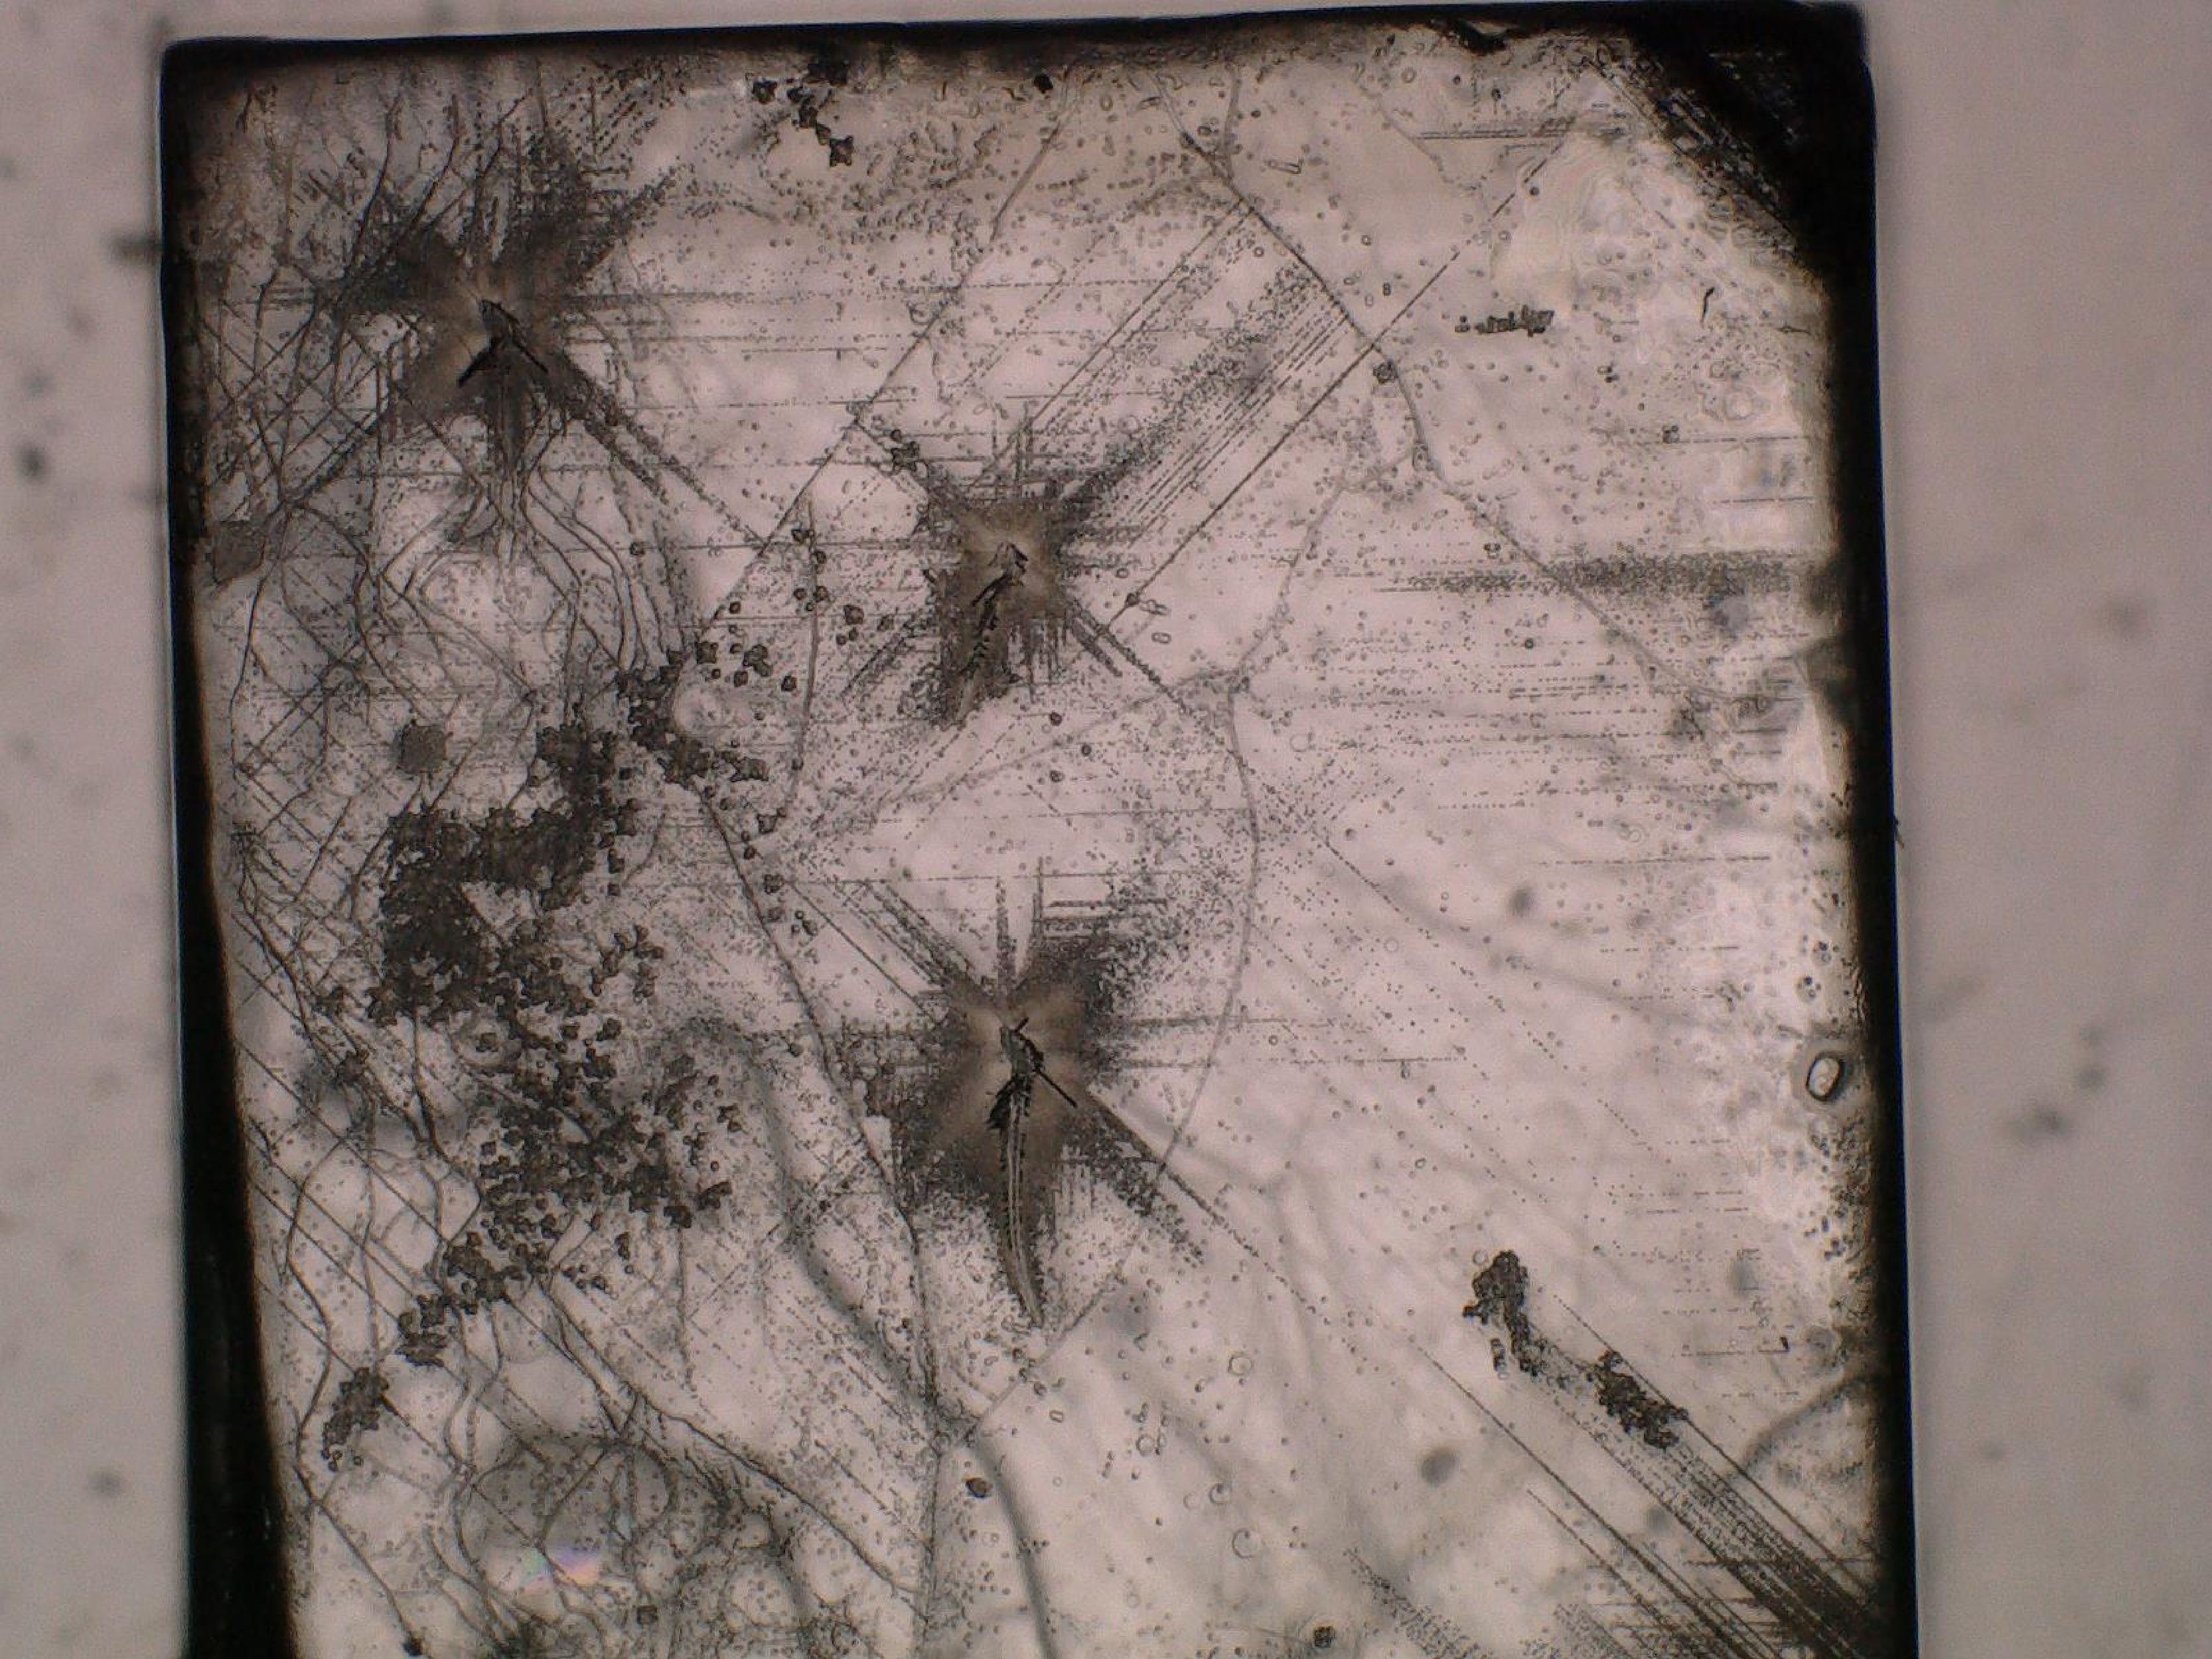
\includegraphics[width=0.7\textwidth]{../media/B2.8/Druck_uebersicht.pdf}
		\caption{Abb. 12}
		\label{abb:Druck all}
	\end{minipage}
	
	\vspace{8pt}
	\begin{minipage}[t]{.5\linewidth}
		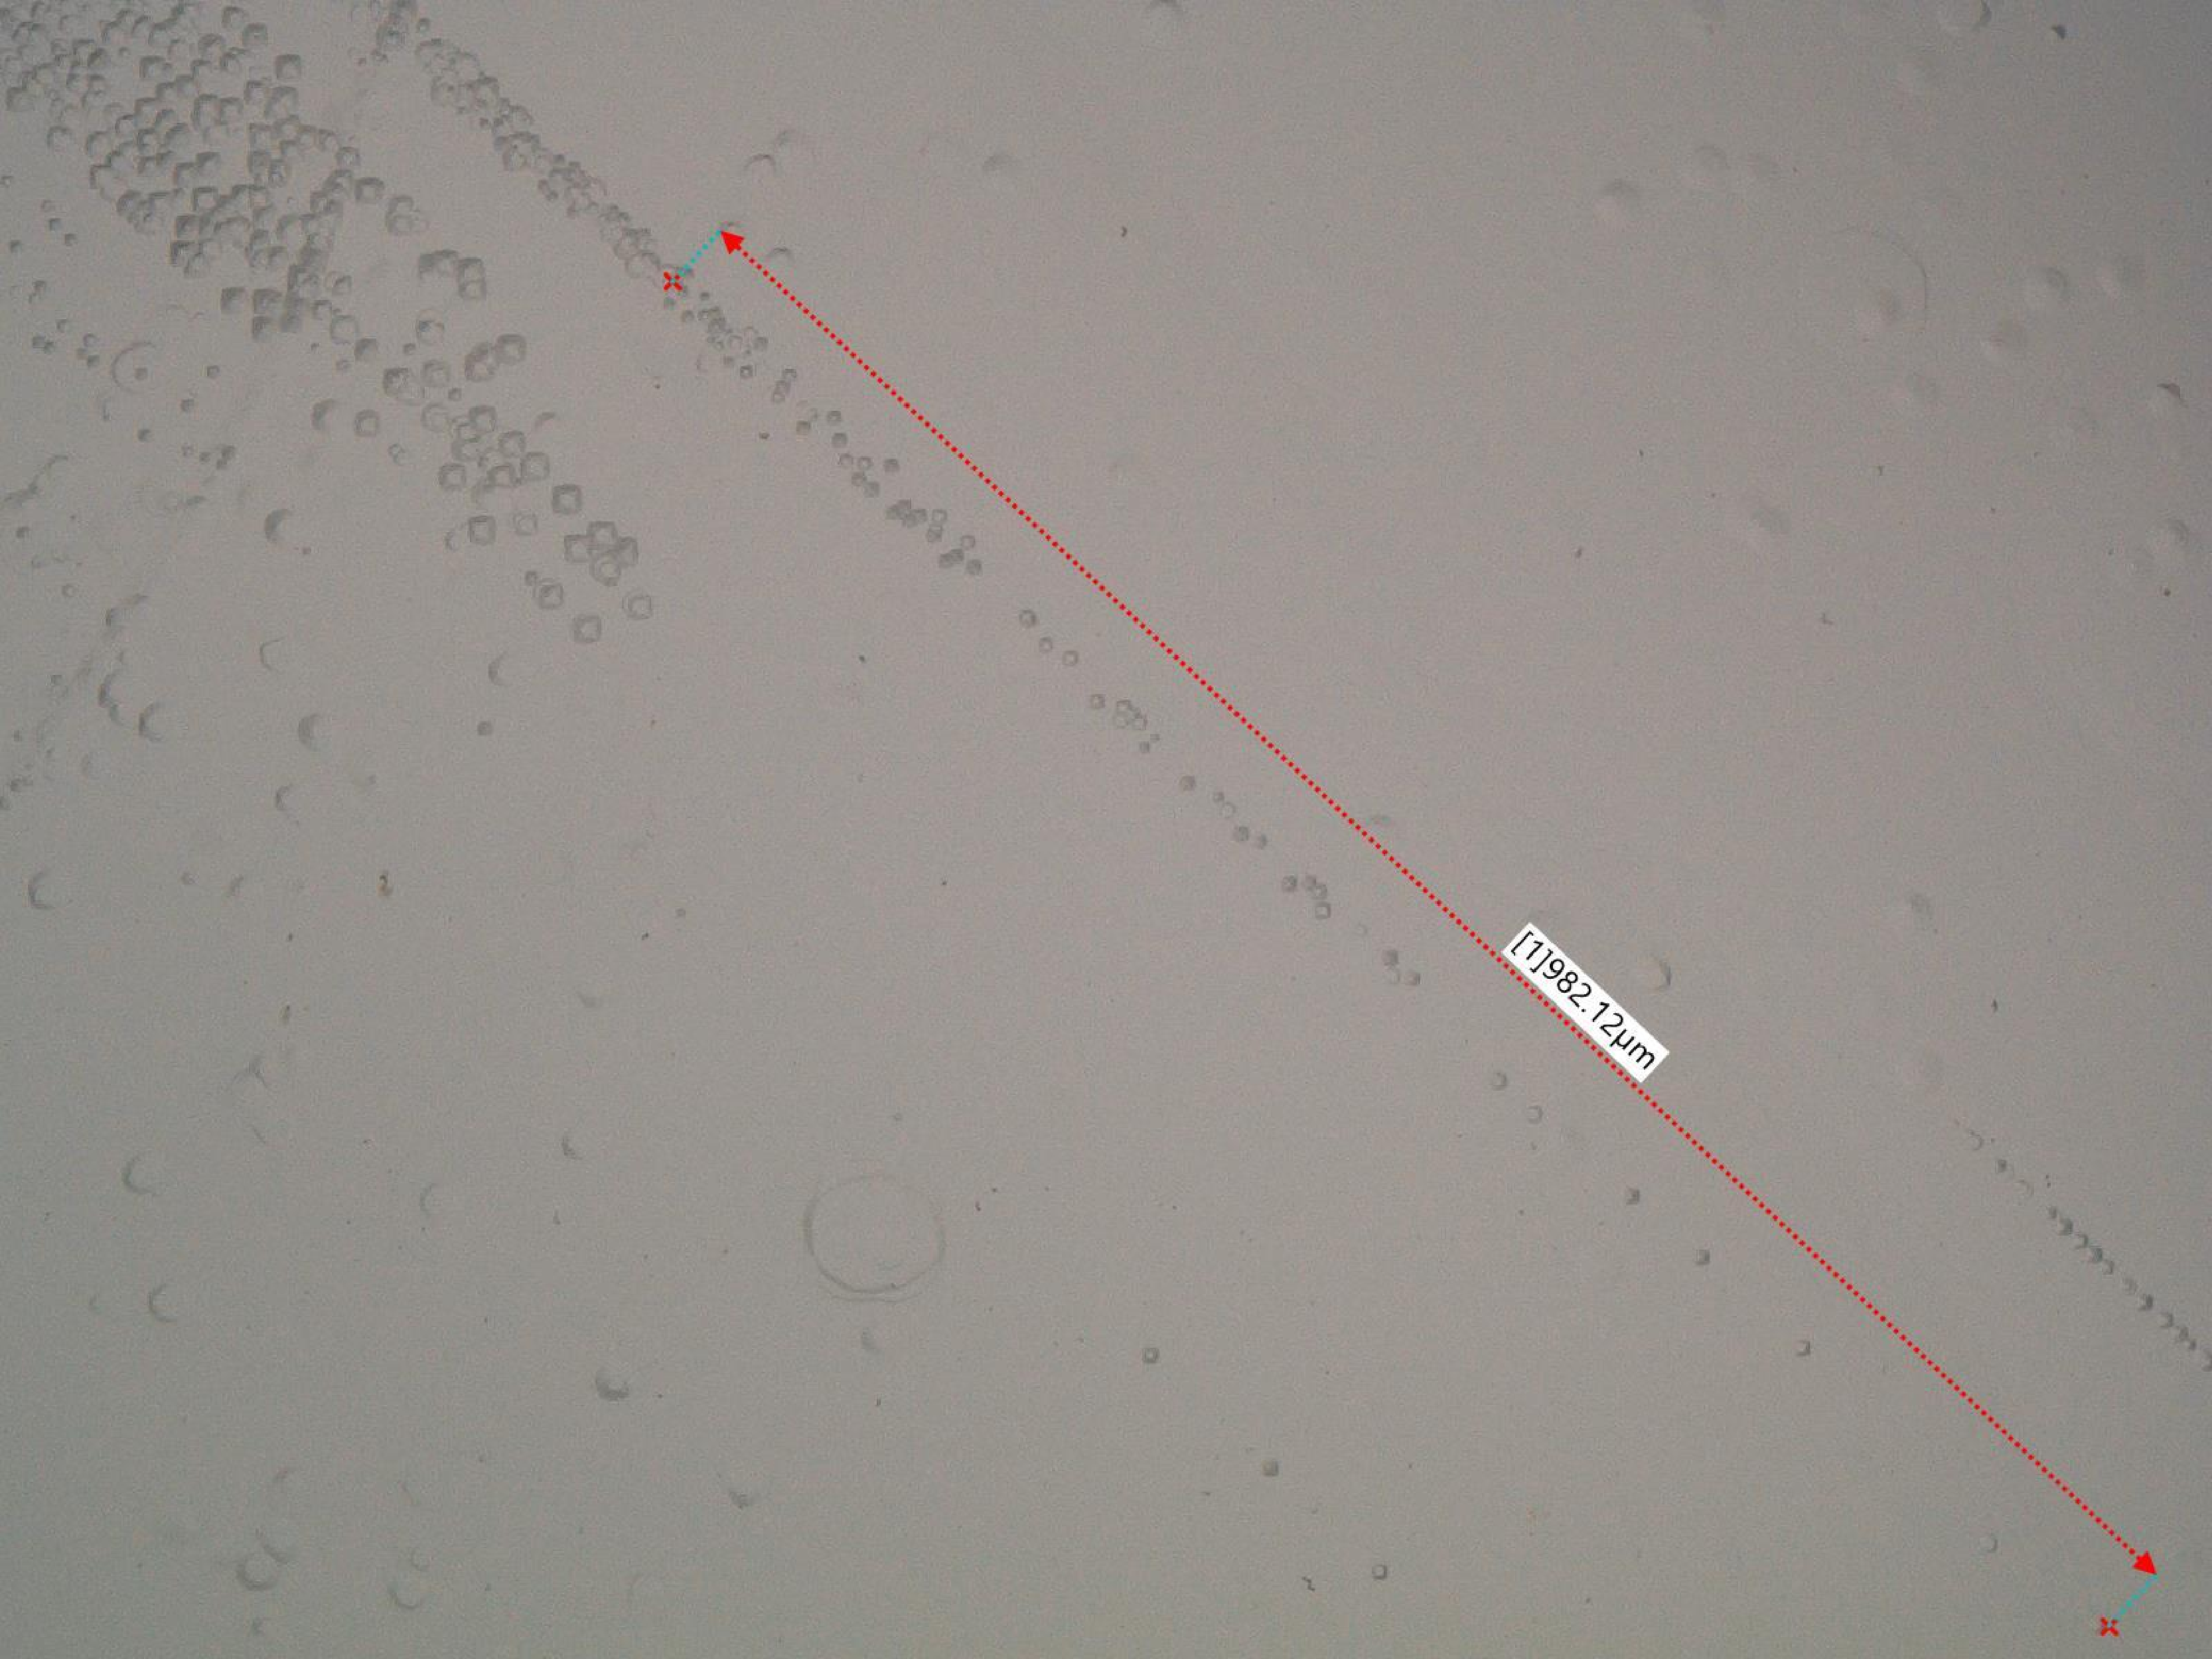
\includegraphics[width=\textwidth]{../media/B2.8/Druck1.pdf}
		\caption{Versetzungswanderung $1$}
		\label{abb:Druck 1}
	\end{minipage}
	\begin{minipage}[t]{.5\linewidth}
		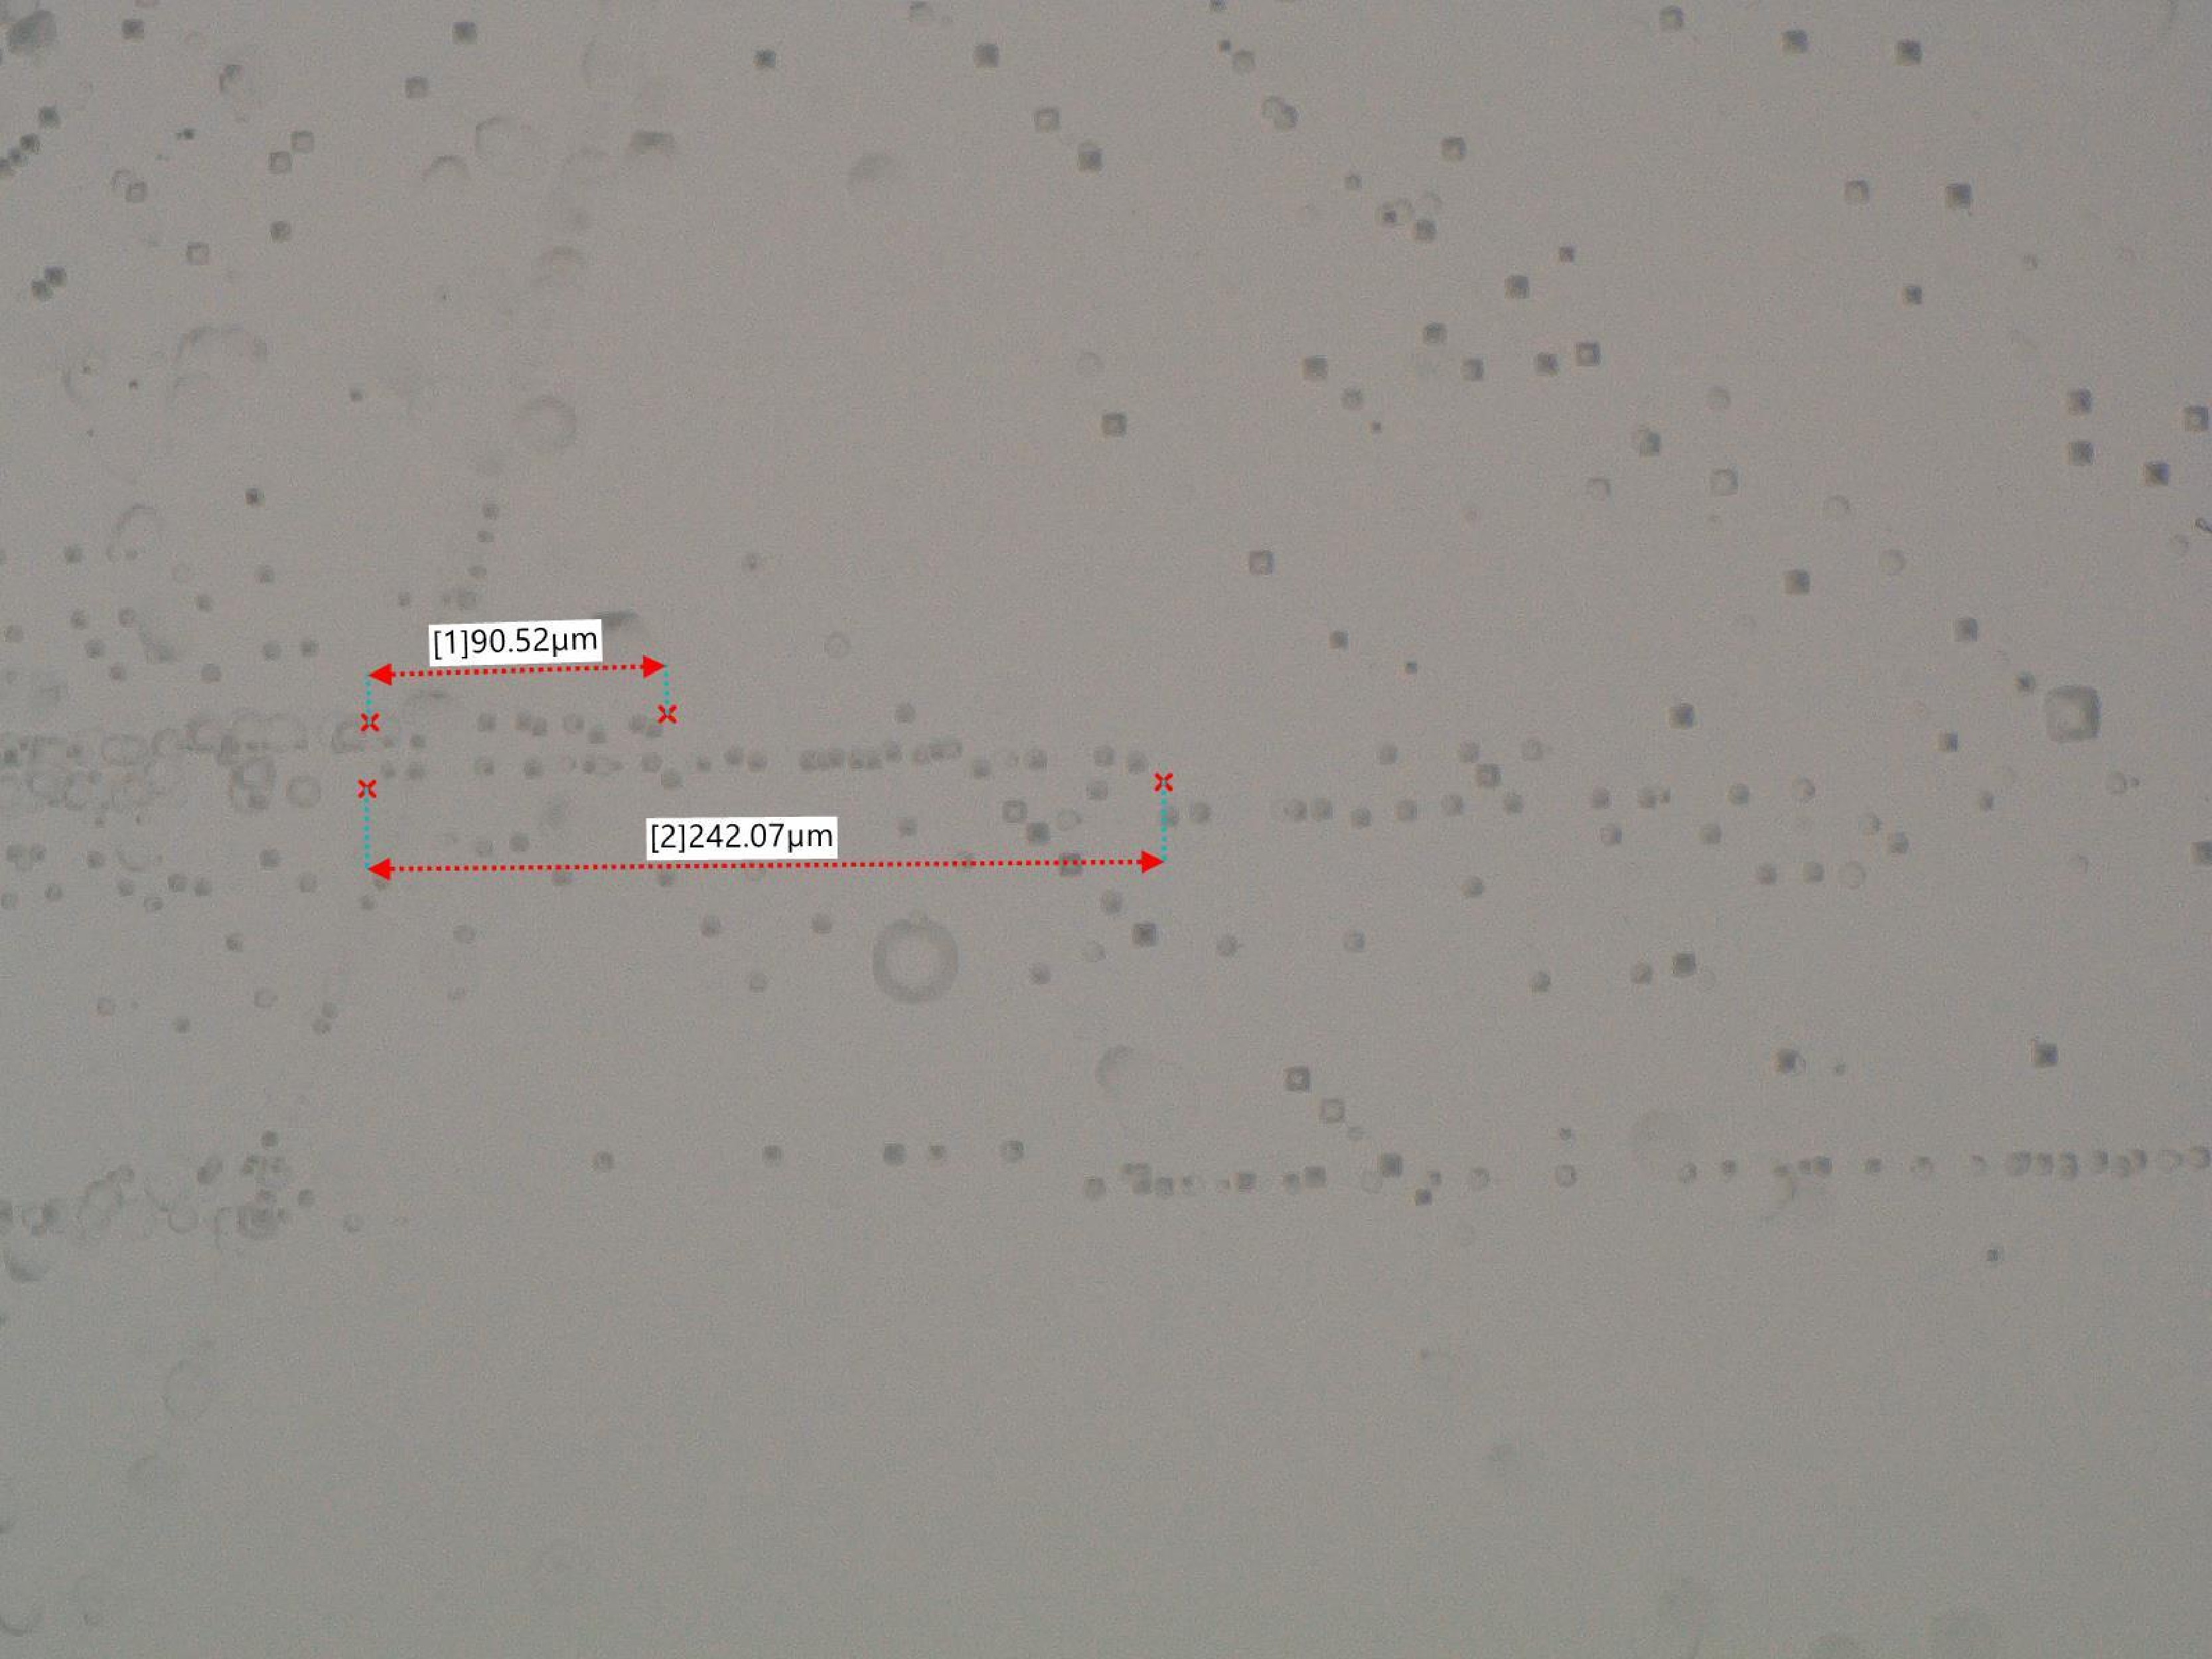
\includegraphics[width=\textwidth]{../media/B2.8/Druck2.pdf}
		\caption{Versetzungswanderung $2$ und $3$}
		\label{abb:Druck 2}
	\end{minipage}
\end{figure}

Die alten Ätzgrübchen kann man von den Neuen unterscheiden, indem man auf die Größendifferenz achtet. Die alten Grübchen existieren länger und wurden somit länger geätzt, während die neuen Grübchen später dazugekommen sind. Dies bedeutet, dass man große und kleine Grübchen unterscheiden kann.

Diesen Unterschied erkennt man in den Abbildungen \ref{abb:Druck 1} und \ref{abb:Druck 2}. So kann man den Abstand der Versetzungswanderung messen und die Geschwindigkeit berechnen.

Die Probe stand für $t=2\mathrm{\,min}$ in einer Presse. Die Strecke
$s$ der Versetzungswanderung wurde durch das Mikroskop ermittelt.
Daraus folgt die Geschwindigkeit $v$ der Versetzungsbewegung.

Der Messfehler für die Zeit durch Start-Stopp-Fehler wird auf
$\Delta t=5\mathrm s$ geschätzt. Weil man die Ätzgrübchen nicht
eindeutig zuordnen und treffen kann, wird der Fehler auf
$0.1\mathrm{\,\mu m}$ geschätzt. Der Fehler $\Delta v$ der
Geschwindigkeit wird durch Gauß'sche Fehlerfortpflanzung ermittelt.

\begin{eqnarray}
    v &=& \frac{s}{t} \\
    \Delta v &=&
        \sqrt{
            \left(\frac{\Delta s}{t}\right)^2
            + \left(\frac{-s \Delta t}{t^2}\right)^2
        }
\end{eqnarray}

\noindent
Auf diese Weise werden die Geschwindigkeiten $v_1$, $v_2$ und
$v_3$ aus den gemessenen Strecken $s_1=982.12\mathrm{\,\mu m}$,
$s_2=90.52\mathrm{\,\mu m}$ und $s_3=242.07\mathrm{\,\mu m}$
ermittelt.

\begin{eqnarray}
    v_1 &=& (8.2 \pm 0.3) \,\frac{\mu m}{s} \\
    v_2 &=& (0.75 \pm 0.03) \,\frac{\mu m}{s} \\
    v_3 &=& (2.02 \pm 0.08) \,\frac{\mu m}{s}
\end{eqnarray}

\noindent
Aufgrund der stark unterschiedlichen Geschwindigkeiten $v_2$ und
$v_3$, die den selben Arm der Rosette beschreiben, werden diese
gemittelt. Die Gewichte $w_i$ folgen aus den Unsicherheiten
$\Delta v_i$. Die resultierende Unsicherheit $\Delta v$ ist entweder
durch die Gauß'sche Fehlerfortpflanzung $\Delta v_\mathrm{G}$ oder
durch die mittlere Quadratsumme der Residuen $\Delta v_\mathrm{MQR}$
zu bestimmen. Hierbei ist der größere Fehler zu wählen.

\begin{eqnarray}
    w_i &=& \frac{1}{(\Delta v_i)^2} \\
    \bar{v} &=& \frac{\sum_{i=2}^{3} v_i\cdot w_i}{\sum_{i=2}^{3} w_i} \\
    \Delta \bar{v}_\mathrm{G} &=&
        \sqrt{\frac{1}{2-1}\frac{\sum_{i=2}^{3}w_i(v_i-\bar{v})^2}{\sum_{i=2}^{3}w_i}} \\
    \Delta \bar{v}_\mathrm{MQR} & = & \frac{1}{\sqrt{\sum_{i=2}^{3}w_i}} \\
    \Delta \bar{v} &=& \max\{\bar{v}_\mathrm{G}, \bar{v}_\mathrm{MQR}\}
\end{eqnarray}

\noindent
Daraus ergibt sich für die Geschwindigkeit $\bar v$ der Rosettenarme
aus Abbildung \ref{abb:Druck 2} wie folgt.

\begin{eqnarray}
    \bar{v} &=& 9.088 \cdot 10^{-7} \frac{m}{s} \\
    \Delta v_\mathrm{G} &=& 4.143 \cdot 10^{-7} \frac{m}{s} \\
    \Delta v_\mathrm{MQR} &=& 8.403 \cdot 10^{-10} \frac{m}{s} \\
    \Rightarrow \bar{v} &=& (0.91 \pm 0.41) \,\frac{\mu m}{s} \\
    v_1 &=& (8.2 \pm 0.3) \,\frac{\mu m}{s}
\end{eqnarray}

\hypertarget{schubspannung}{%
\subsection{Schubspannung}\label{schubspannung}}

Zuletzt soll wir die Schubspannung im Gleitsystem der Versetzungen durch
den Druck bestimmt werden.

Dazu wird der Druck $p$ der Presse, welcher auf die Probe wirkte,
benötigt. Dieser wird durch die Gewichtskraft $F_G=mg$ beschrieben,
wobei $m$ die Masse und $g$ die Erdbeschleunigung sind. Desweiteren
ist die Oberfläche $A=9,073,890.26\mathrm{\,\mu m^2}$, auf die diese
Kraft wirkte, benötigt. Diese wurde durch das Mikroskop vermessen, siehe
Abbildung \ref{abb:Querschnitt}.

\begin{eqnarray}
    p &=& \frac{mg}{A} \label{Druck}
\end{eqnarray}

\begin{figure}[ht]
	\centering
	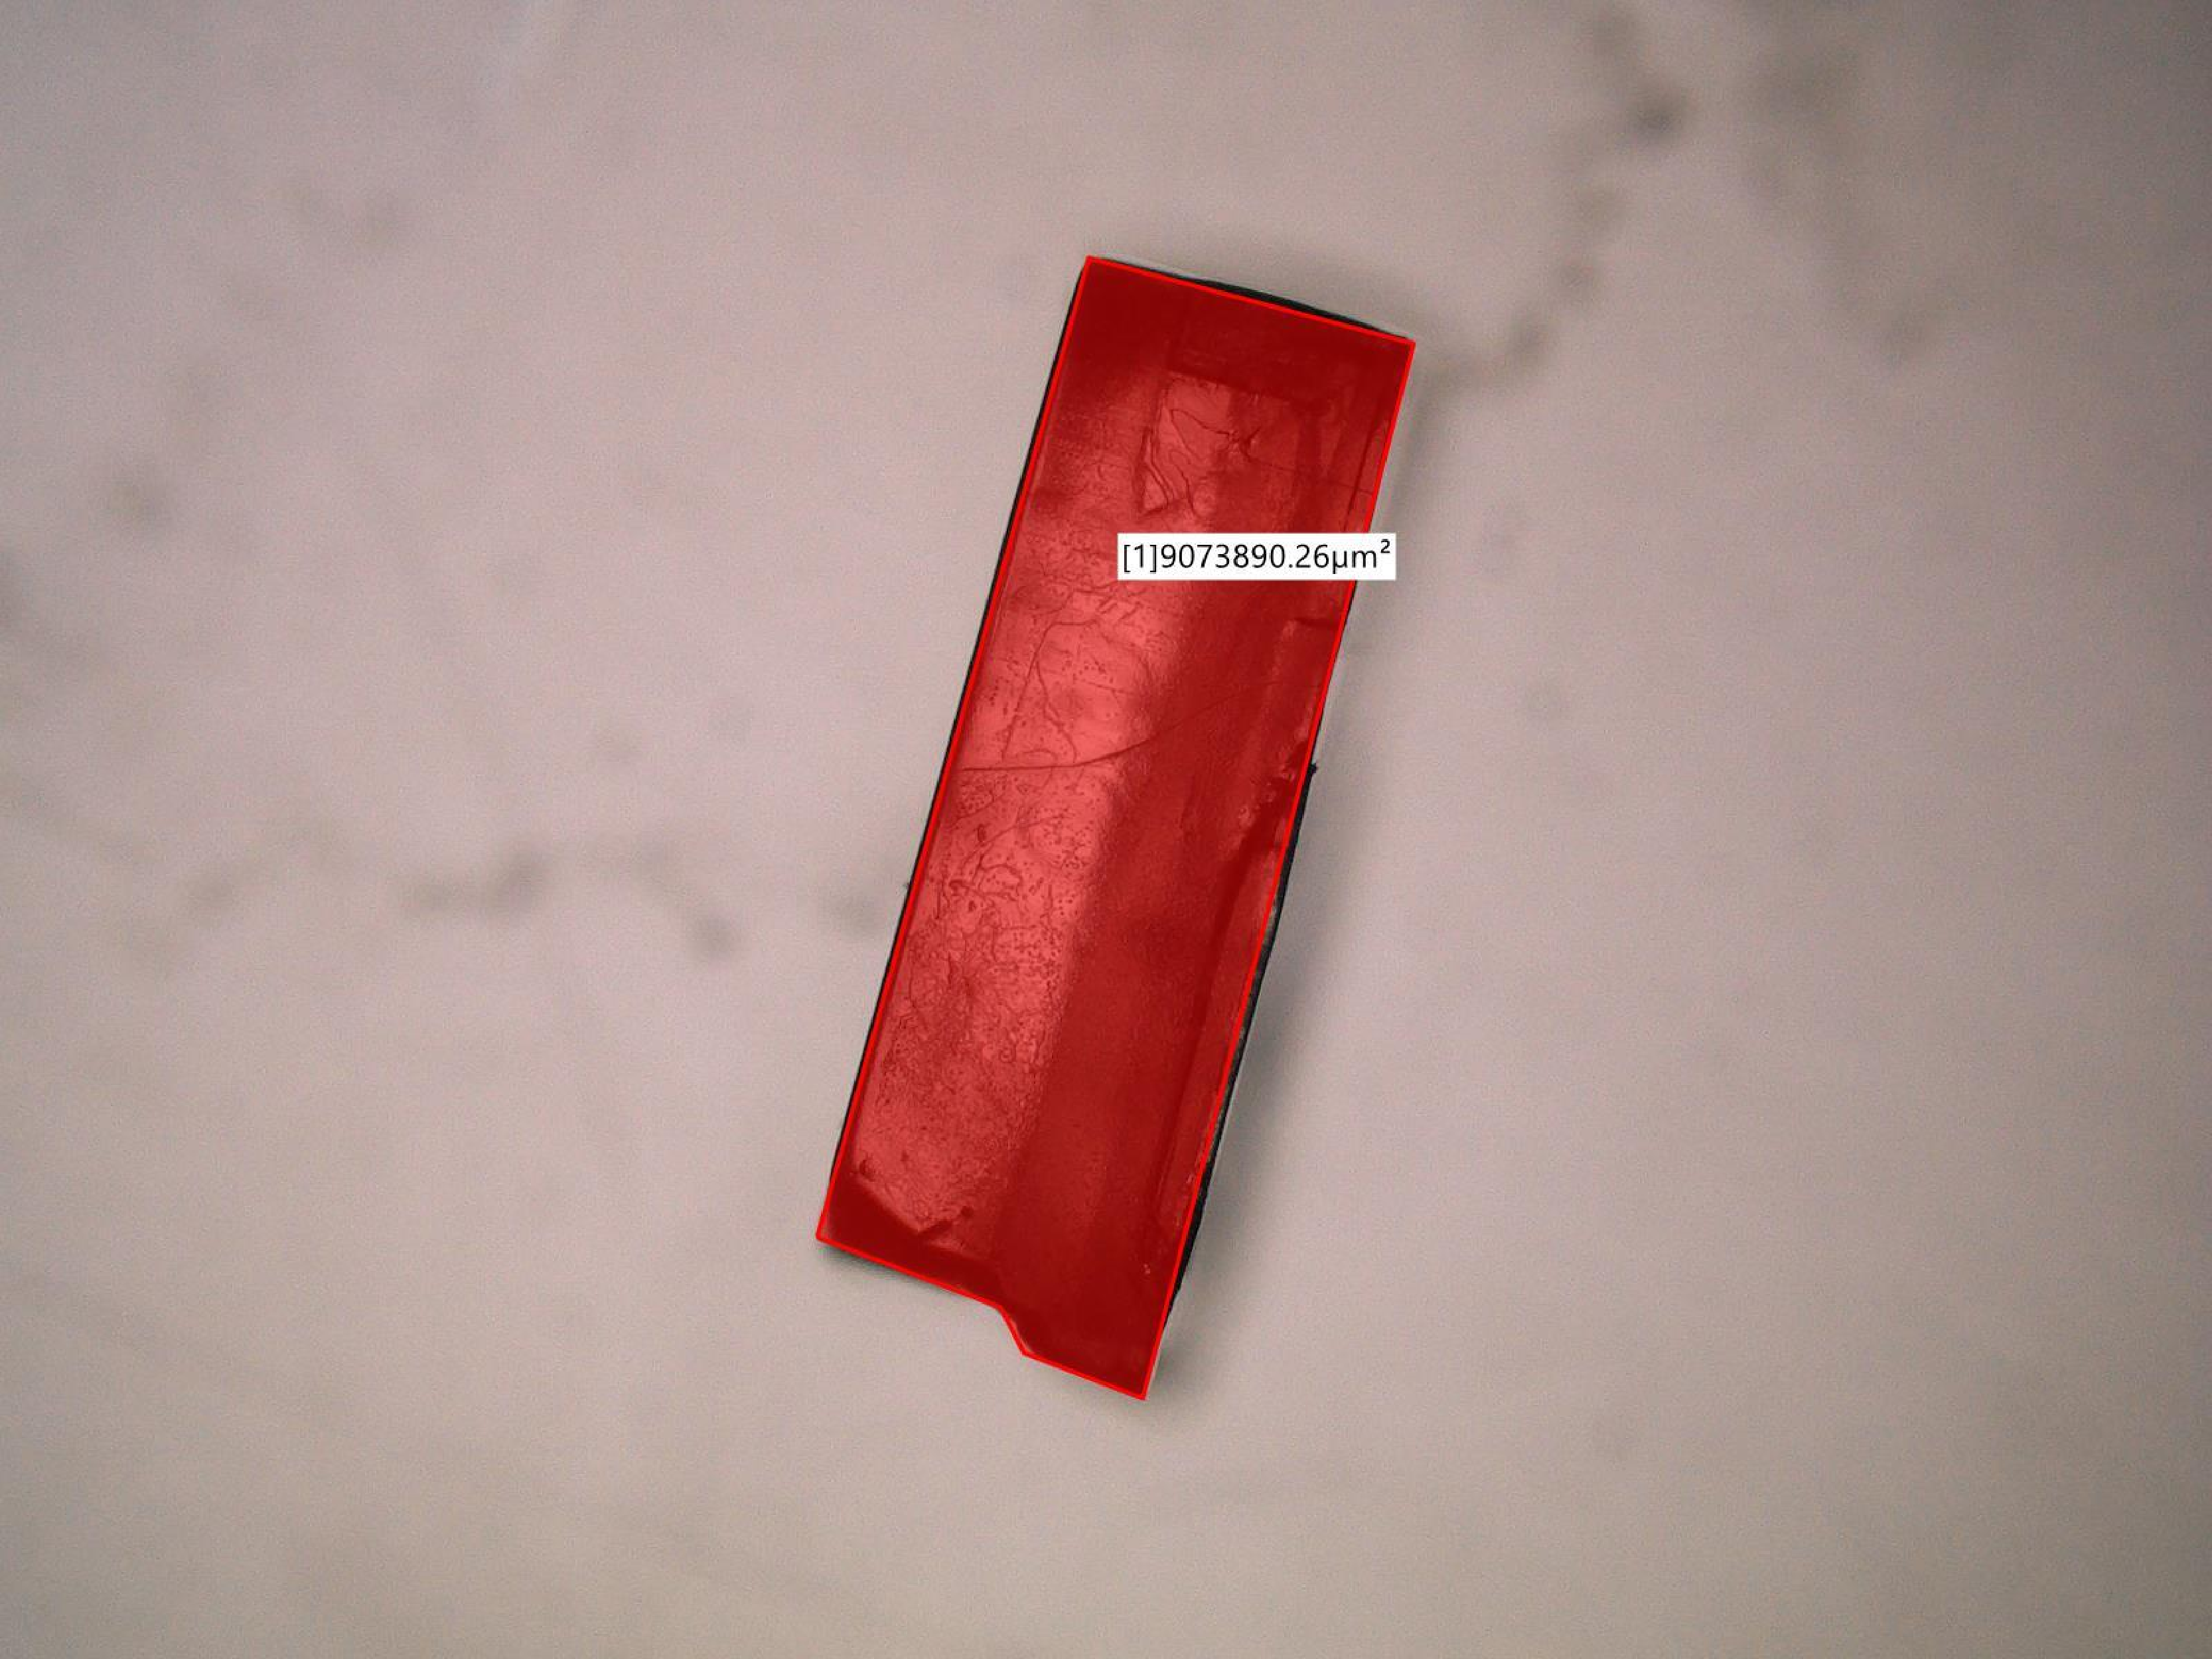
\includegraphics[width=0.7\textwidth]{../media/B2.8/Querschnittsflaeche_tempered.pdf}
	\caption{Oberfläche der eingespannten Probe}
	\label{abb:Querschnitt}
\end{figure}

\noindent
Der Deckel der Presse hat ein Gewicht von $948\mathrm{\,g}$,
zusätzlich wurde ein $841\mathrm{\,g}$ schweres Gewicht darauf gelegt.
Diese Werte wurden als fehlerfrei angenommen. Da die Probe nicht gerade
in der Presse stand und man möglicherweise die Fläche nicht exakt
trifft, wird der Fehler der Fläche als $100\mathrm{\,\mu m^2}$
abgeschätzt. Dadurch kann die Unsicherheit $\Delta p$ durch Gleichung
$\eqref{DeltaDruck}$ beschrieben werden.

\begin{eqnarray}
    \Delta p &=& \frac{mg \Delta A}{A^2} \label{DeltaDruck}
\end{eqnarray}

\noindent
Die Schubspannung $\sigma$ setzt sich aus der tangentialen
Kraftkomponente und der Schnittfläche der
$\lbrace1\,1\,0\rbrace$-Ebenen zusammen, vergleiche Abbildung \ref{abb:Gleitebene}. Der Kristall verschiebt
sich in einem Winkel von
$\varphi=45\,^\circ=\frac{\pi}{4}\mathrm{\,rad}$ entlang der
$\lbrace1\,1\,0\rbrace$-Ebenen. Daher kann die Schubspannung
$\sigma$ aus dem Druck $p$ berechnet werden.

\begin{eqnarray}
    \sigma &=& \frac{F_G \cdot \cos(\varphi)}{\frac{A}{\cos(\varphi)}}\\
        &=&\frac{F_G}{A} \cdot \cos^2(\varphi) \\
        &=& \frac{1}{2}\frac{F_g}{A}\\
    \sigma &=& \frac{p}{2} \\
    \Delta \sigma &=& \frac{\Delta p}{2}
\end{eqnarray}

Mithilfe der Gleichungen $\eqref{Druck}$ und $\eqref{DeltaDruck}$
lässt sich die Schubspannung $\sigma$ ermitteln.

\begin{eqnarray}
    p &=& (1,934.13 \pm 0.02) \mathrm{\,kPa} \\
    \sigma &=& 967.07 \pm 0.01 \mathrm{\,kPa}
\end{eqnarray}

\hypertarget{fazit}{%
\section{Fazit}\label{fazit}}

Es ist schwierig, die Ergebnisse konkret zu bewerten, denn es gibt keine
Literaturwerte zum Vergleich. Daher kann die Bewertung nur qualitativ
erfolgen. Dies macht eine Bewertung der Schubspannung extrem schwierig,
weshalb diese hier nicht erfolgt.

Alle drei ermittelten Kleinwinkelkorngrenzen auf der getemperten Probe
hatten einen Winkel im Bereich von einigen Milligrad. Damit fallen sie
alle deutlich in den Bereich einer Kleinwinkelkorngrenze, wodurch die
hier getätigte Kleinwinkelannahme gerechtfertigt ist.

\hypertarget{uxe4tzgruxfcbchendichte-1}{%
\subsection{Ätzgrübchendichte}\label{uxe4tzgruxfcbchendichte-1}}

Die großen Fehler in den Mittelwerten der Ätzgrübchendichten folgen
daraus, dass nur zwei typische Stellen pro Probe verwenden um die
durchschnittliche Ätzgrübchendichte der gesamten Probe zu bestimmen. Die
Ergebnisse sind trotzdem gut interpretierbar.

Es wurde erwartet, dass die Ätzgrübchendichte und damit die
Versetzungsdichte der getemperten Probe niedriger ist als die der nicht
getemperten Probe, da sich die Versetzungen in der Probe beim
Temperungsprozess auslöschen. \cite{Newey}

Diese Messungen stellen aber das Gegenteil dar. Die Ätzgrübchendichte
der getemperten Probe ist mit ca.
$\bar N_\mathrm{t}=(8.3\pm 5.5) \cdot 10^4 \mathrm{\, cm^{-2}}$ selbst
innerhalb der Fehlergrenzen größer als die Ätzgrübchendichte der nicht
getemperten Probe
$\bar N_\mathrm{nt}=(1.4 \pm 1.2) \cdot 10^4 \mathrm{\, cm^{-2}}$.

Dies kann mehrere Ursachen haben. Die erste Möglichkeit ist, dass unsere
ausgesuchten repräsentativen Stellen doch nicht so repräsentativ sind
wie wir dachten. Wir hätten z.B. aus Versehen eine oder beide Stellen
der getemperten Probe innerhalb einer stark beschädigten Zone wählen
können.

Dies führt direkt zur zweiten Möglichkeit. Es kann sein, dass die
getemperte Probe nach dem Tempern beschädigt wurde und so neue
Versetzungen hinzukamen. Dies kann beispielsweise durch Abrutschen der
Probe aus der Pinzette, insbesondere beim Spülen, passiert sein.

In beiden Fällen ist das gemessene Ergebnis nicht undenkbar, wenn auch
unerwartet. Der Effekt des Temperns auf die Ätzgrübchendichte der Probe
konnte somit zwar nicht beobachtet werden. Dennoch konnte ein Gefühl für
die Menge an Versetzungen in $\mathrm{LiF}$ entwickelt werden.

\hypertarget{rosetten}{%
\subsection{Rosetten}\label{rosetten}}

Auf den Horizontalen und Vertikalen sind die Versetzungsarme deutlich
weniger ausgeprägt als auf den Diagonalen. Dies liegt dran, dass der
kürzeste Burgersvektor in den $\expval{1\,1\,0}$-Richtungen zeigt. In
diesen Richtungen treten auch die Stufenversetzungen auf. Die weniger
ausgeprägte Arme zeigen in den $\expval{1\,0\,0}$-Richtungen, wo sich
Schraubenversetzungen bewegen. Diese Richtungen haben den zweitkürzesten
Burgersvektor und haben damit die zweitniedrigste Bindungsenergie.

Die Ergebnisse entsprechen die Theorie und unsere Erwartung.

Man sieht, dass die Versetzung von dem Arm in Abbildung \ref{abb:Druck 1} mit
Geschwindigkeit $v_1=(8.2 \pm 0.3) \,\frac{\mu m}{s}$ deutlich
schneller als die von dem Arm in Abbildung \ref{abb:Druck 2} mit der
Geschwindigkeit $\bar{v}=(0.91 \pm 0.41) \,\frac{\mu m}{s}$ gewandert
ist.

\clearpage
\hypertarget{literaturverzeichnis}{%
	\section{Literaturverzeichnis}\label{literaturverzeichnis}}
\renewcommand{\section}[2]{} % remove extra title
\begin{thebibliography}{9}
\bibitem{Newey}
	 C. Newey und R. Davidge, ``Dislocations in Lithiumfluoride'', editiert von
	A. Bailey, Online verfügbar unter
	\url{https://ph2.uni-koeln.de/fileadmin/Lehre/PraktikumB/Dislocations_in_Lithium_Fluoride.pdf}, 1965
	\bibitem{Kittel}
	C. Kittel, ``Einführung in die Festkörperphysik'', Oldenbourg Verlag, 2005
\bibitem{Hunklinger}
	S. Hunklinger, ``Festkörperphysik'', Oldenbourg Verlag, 2011
\bibitem{Gross}
	R. Gross und A. Marx, ``Festkörperphysik'', Oldenbourg Verlag, 2012
\bibitem{Uni}
	Universität zu Köln, ``Anleitung zum Versuch 2.8 -- Versetzungen in
	LiF'', Online verfügbar unter
	\url{https://ph2.uni-koeln.de/fileadmin/Lehre/PraktikumB/B28-LiF_tutorial_de.pdf}, Juni 2013
\end{thebibliography}
\end{document}
